%%%%%%%%%%%%%%%%%%%%%%%%%%%%%%%%%%%%%%%%%%%%%%%%%%%%%%%%%%%%%%%%%%% 
%                                                                 %
%                      THESIS MAIN FILE                           %
%                                                                 %
%%%%%%%%%%%%%%%%%%%%%%%%%%%%%%%%%%%%%%%%%%%%%%%%%%%%%%%%%%%%%%%%%%% 

% document definition 
\documentclass[a4paper,11pt,chap, twoside, openright]{report}
\usepackage[hmarginratio=3:2]{geometry}
% Use the first command below if you want captions over 1 line indented. A side
% effect of this is to remove the use of bold for captions. To restore bold,
% also include the second line below.


\newcommand{\PaperTitle} {Probabilistic Learning of Object Locations based on spatio-temporal information }
\newcommand{\PaperSubject} {Predictive model of object locations in environment}
\newcommand{\PaperTerm} {Summerterm 2016}		
\newcommand{\PaperDate} {\today}			
\newcommand{\ThesisAdvisor} {Tim Niemueller }			
\newcommand{\ThesisReferee} {Prof. Dr. Paul Pl\"{o}ger}
\newcommand{\ThesisExReferee} {Prof. Dr. Gerhard Lakemeyer }
\newcommand{\PaperLecturerEMail} {mailto:advisor@xyz}
\newcommand{\Paperkeywords} {key1, key2, key3}		
\newcommand{\PaperMainWriter} {Deebul Nair}
\newcommand{\PaperMainWriterEMail} {mailto:deebul.nair@smail.inf.fh-bonn-rhein-sieg.de}
\newcommand{\ThesisAuthor} {Deebul Nair}

%\usepackage[latin1]{inputenc} 

\usepackage{enumitem}
\usepackage[table]{xcolor} 
%\usepackage{graphicx}
\usepackage{color} 
\usepackage{placeins}
\usepackage{transparent} 
\usepackage{hyperref}
\usepackage{tabto}


\usepackage[final]{graphicx}
%\usepackage{epstopdf}
\usepackage{url}
%\usepackage[expert,vargreek]{lucidbrb}

%\usepackage{mya4page} % not used, because now is implemented in the class 
\usepackage{amsmath}
%\usepackage{hyperref}
\usepackage{bibnames}
\usepackage{path}
%\usepackage{subfigure}

\usepackage{caption}
\usepackage{subcaption}


\usepackage{amsmath}
\usepackage{todonotes}

\usepackage{tikz}
\usepackage{amsmath}
\usetikzlibrary{bayesnet}
\usepackage{tabularx}
\usepackage{placeins}
\usepackage{pstricks}
\usepackage[titletoc]{appendix}
\usepackage{setspace}


\usepackage[nottoc]{tocbibind}
%\usepackage{footmisc}
%\usepackage[perpage,symbol*]{footmisc} 


%---------------------------------------------------------------
\usepackage{color}
\definecolor{listinggray}{gray}{0.9}
%---------------------------------------------------------------
%\usepackage[copy=false, edit=false]{pdfcrypt}

%---------------------------------------------------------------
\usepackage{listings}
\lstset{language=Java}
\lstset{basicstyle=\footnotesize\small,%ttfamily,%\small,
tabsize=4,
tab=$\to$,
float=tbph,
extendedchars=true,
breaklines,
% prebreak={\space\MyHookSign},
% frame=single,
showtabs=false,
showspaces=false,
showstringspaces=false,
keywordstyle=\color{red}\bfseries,
identifierstyle=\bf\ttfamily,
aboveskip=\bigskipamount,
}
\lstset{captionpos=b}
\lstset{keywordstyle=\color{blue}\bfseries\bf}
\lstset{backgroundcolor=\color{listinggray}, rulecolor=\color{blue}}
\lstset{linewidth=\textwidth}
\lstset{stepnumber=5}
\lstset{numbers=left}
\lstset{numberstyle=\tiny\color{blue}}
\lstset{commentstyle=\color{magenta}\textit, stringstyle=\upshape,
	showstringspaces=false}
\lstset{frame=trBL,frameround=tttt}
%---------------------------------------------------------------

%% Hyperref setup
\usepackage{hyperref}
\hypersetup{
	 a4paper,
   colorlinks=true,
   linkcolor=black,
   filecolor=black,
   citecolor=black,
   urlcolor=black,
   plainpages=false,
   pdftitle={ \PaperTitle },
   pdfsubject={ \PaperSubject },
   pdfauthor={ \ThesisAuthor <deebul.nair@smail.inf.h-brs.de>},
   pdfkeywords={ \Paperkeywords },
   bookmarksnumbered=true,
   pdfpagemode=UseOutlines,
   pdfpagelayout=SinglePage,  
   bookmarksopen=true
}
%\usepackage[copy=true, edit=false, annotate=true]{pdfcrypt}

\usepackage{fancyhdr}
\setlength{\headheight}{15pt}

\pagestyle{fancy}
\renewcommand{\chaptermark}[1]{ \markboth{#1}{} }
\renewcommand{\sectionmark}[1]{ \markright{#1} }

\fancyhf{}
\fancyhead[LE,RO]{\thepage}
\fancyhead[RE]{\textit{ \nouppercase{\leftmark}} }
\fancyhead[LO]{\textit{ \nouppercase{\rightmark}} }

\fancypagestyle{plain}{ %
  \fancyhf{} % remove everything
  \renewcommand{\headrulewidth}{0pt} % remove lines as well
  \renewcommand{\footrulewidth}{0pt}
}


\begin{document}
\pagenumbering{gobble}

% Declare new goemetry for the title page only.
%\newgeometry{margin=1.4in}
\begin{titlepage}
\raggedright
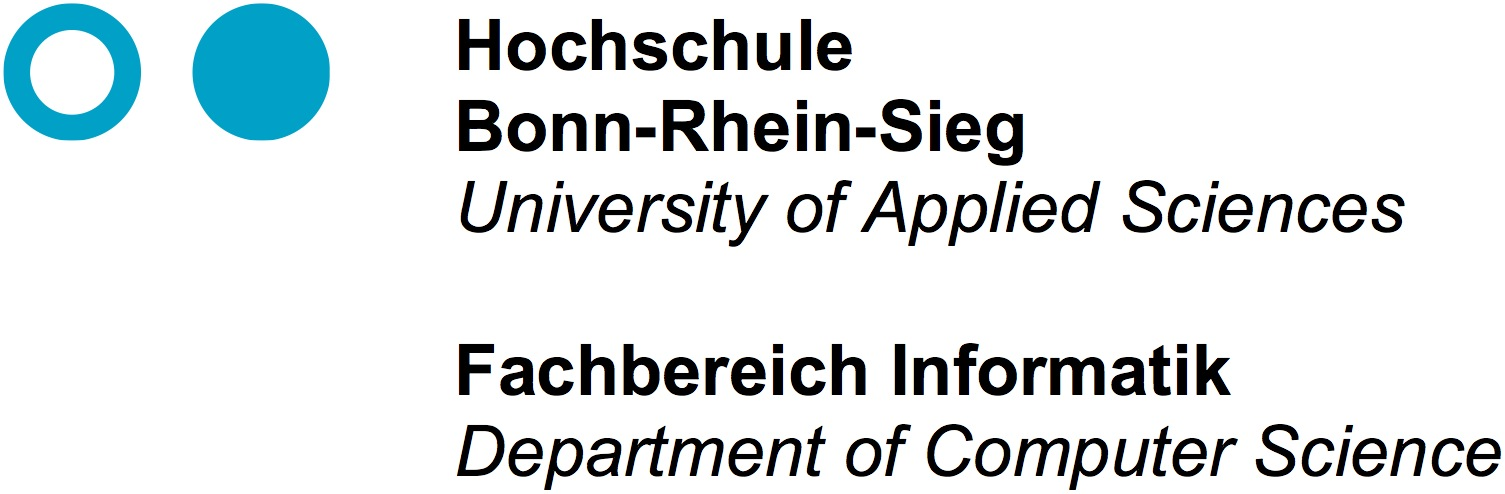
\includegraphics[width=0.4\textwidth]{pictures/FH-Header.jpg}\\
\centering
\vspace*{1in}
\begin{Large}\bfseries
\PaperSubject \par
\end{Large}
\vspace{1.2in}
\begin{LARGE}\bfseries
 \par
\end{LARGE}
\vspace{0.5in}
\begin{large}
\PaperMainWriter%\href{\PaperMainWriterEMail}{\PaperMainWriter \footnote{\href{\PaperMainWriterEMail} {santosh.thoduka@smail.inf.fh-bonn-rhein-sieg.de}}}
 \par
\end{large}
\vspace{0.5in}
A thesis submitted in partial fulfilment of the requirements for the degree of
Master of Science in Autonomous Systems \\
at Bonn-Rhein-Sieg University of Applied Sciences
\vfill
\vspace{0.5in}
\par
\vfill
Thesis Supervisors:\\
\ThesisReferee \\ %\href{\PaperLecturerEMail}{\PaperLecturer \footnote{\href{\PaperLecturerEMail} {paul.ploeger@h-brs.de}}}\\
\ThesisExReferee \\ % \href{\SecondSupervisorEMail}{\SecondSupervisor \footnote{\href{\SecondSupervisorEMail} {gerhard.kraetzschmar@h-brs.de}}}\\
\ThesisAdvisor \\
\vspace{0.4in} %\href{\ThirdSupervisorEMail}{\ThirdSupervisor \footnote{\href{\ThirdSupervisorEMail} {frederik.hegger@h-brs.de}}}
September 2016

\end{titlepage}




   
\cleardoublepage
\onehalfspacing
\pagenumbering{roman}
\cleardoublepage
\thispagestyle{empty}
\hbox{}
\vfill
\noindent
I, Deebul Nair Sivarajan, declare that this work has not previously been submitted to this or any other university and that, unless otherwise stated, it is entirely my own work.
\vskip 60pt

\hrule width 2.5cm
\hfill \hspace{5cm}
\hrulefill
\vskip -4pt
\leftline{\hspace{0.6cm} Date \hfill Signature \hspace{1.1cm}}   

\clearpage
\cleardoublepage
%%%%%%%%%%%%%%%%%%%%%%%%%%%%%%%%%%%%%%%%%%%%%%%%%%%%%%%%%%%%%%%%%%% 
%                                                                 %
%                            ABSTRACT                             %
%                                                                 %
%%%%%%%%%%%%%%%%%%%%%%%%%%%%%%%%%%%%%%%%%%%%%%%%%%%%%%%%%%%%%%%%%%% 
\begin{abstract}


In the future, we envison domestic robots to provide useful services both in domestic as well as in industrial context. Examples include domestic service robots, that implements large part of our housework, versatile assistants, that provide automation, transportationm inspection and monitoring services. The challenge in these aplications is that the robots has to have lot of information and knowledge about the user and environment to operate under complete autonomy.This thesis aim is to enable domestic robots to acquire knowledge about behaviour and preferences of the users around them. The developed approaches in this thesis cover the following two topics: (1) learning about the temporal human location behvaiour in-door using previously observed locations of the human (2) learning user preference in object placement. 
 
All techniquies developed in this thesis are based on probabilistic bayesian learning and inference. They have been implemented and evaluated on datasets  collected using real robots as well as on simulated datasets. Extensive experiments have been conducted to evaluate the and validate the properties of the proposed models.
\todo{need to be revised completely}
\end{abstract}
\cleardoublepage
%%%%%%%%%%%%%%%%%%%%%%%%%%%%%%%%%%%%%%%%%%%%%%%%%%%%%%%%%%%%%%%%%%% 
%                                                                 %
%                         ACKNOWLEDGEMENT                         %
%                                                                 %
%%%%%%%%%%%%%%%%%%%%%%%%%%%%%%%%%%%%%%%%%%%%%%%%%%%%%%%%%%%%%%%%%%% 
 
\specialhead{ACKNOWLEDGMENTS}
 
ACK. ACK. ACK. here you can write your acknowledgements. 

\cleardoublepage
% Ends the declared geometry for the titlepage
\restoregeometry
%--------------------------

\onehalfspacing
\tableofcontents
\cleardoublepage
\listoffigures
\cleardoublepage
\section*{Abbreviations}
%\addcontentsline{toc}{chapter}{Abbreviations}
\NumTabs{4}
FDR \tab{False Discovery Rate}\\
FN \tab{False Negative}\\
FOE \tab{Focus Of Expansion}\\
FP \tab{False Positive}\\
GPU \tab{Graphics Processing Unit}\\
GT \tab{Ground Truth}\\
HMM \tab{Hidden Markov Models}\\
IMO \tab{Independently Moving Object}\\
MAD \tab{Median Absolute Deviation}\\
MDO \tab{Motion Detection Output}\\
OMS \tab{Object Motion Sensitive}\\
PCA \tab{Principal Component Analysis}\\
PCL \tab{Point Cloud Library}\\
RANSAC \tab{RANdom SAmple Consensus}\\
ROS \tab{Robot Operating System}\\
SLIC \tab{Simple Linear Iterative Clustering}\\
SVD \tab{Singular Value Decomposition}\\
TP \tab{True Positive}\\
TPR \tab{True Positive Rate}\\
TTC \tab{Time To Collision}\\
\cleardoublepage
% the main contents %
\pagenumbering{arabic}
\chapter{Introduction}


For robots to make a smooth ingress into dynamic human environments like home and office, the robots need to be able to close the \emph{perceive-action-learning} loop. Essentially these domestic service robots should perceive the environment, interact with the environment, learn from experiences and repeat. The robot interacts with the environment by choosing a sequence of low-level actions . For example, lets take the high-level task of ``making tea", this will require the following actions to be executed sequentially: fill the kettle, boil water, find the teabag, find a cup, put teabag into the cup and pour hot water into the cup. But for executing some of the actions like finding the kettle, finding teabag, finding cup etc. requires the robot to have prior knowledge about the possible locations. Such knowledge about the environment or the user needs to be learned by the robot. The goal of this thesis is to enable domestic service robots to gain knowledge about common behaviours and preferences of the user in a non-intrusive manner. Specifically, we address how Bayesian methods can be used to provide a flexible and computationally efficient structure for acquiring knowledge using limited spatio-temporal information collected by these service robots.

Domestic service robots need to have the ability to automatically and quickly adapt to a new environment. Imagine if the robot could learn how the user arranges the breakfast table by looking at the data from previous days? Robots can observe our lives and provide small insights the user doesn’t even notice. The robots can pass along helpful information to the users, like observing their sleep habits and tell us when we are not having adequate sleeps. By learning how the user interacts with their homes and how they live their lives, robots will be able to provide better services to their users. 


Domestic service robots while interacting with the user and environment produce information which after being processed in perception, actuation, or decision making are discarded. \cite{niemueller2012generic} has proposed an approach of storing these information in a robot database and produce useful knowledge. 
The domestic robot will continuously record sightings of objects and persons with position and time in a database to form the spatio-temporal robot memory. Machine learning is a good method for automatic knowledge generation from the stored information. But in order to adapt quickly the robot needs to able to extract valuable knowledge from small amount of information, i.e., the learning algorithms need to be data efficient.

To illustrate the relevance of the topics presented in this thesis, we motivate our work using a typical task of a domestic service robot.   We assume that the robot is given the task of ``making coffee" for the user Waldo, which requires the robot to locate the coffee cup of Waldo first, make coffee and then to locate Waldo for delivering it to him. To begin the search for the coffee cup, it would help the robot to have some prior knowledge regarding Waldo's habits; in particular the typical locations where he keeps his cup. This enables the robot to funnel its search for the object from a large number of locations to the most probable ones. Once the coffee cup is located and grasped the robot needs to reason about where it can currently find Waldo for delivering it to him. This in turn, requires the robot to have knowledge about the likely locations of Waldo at that time.

This motivating example leads us to the two research topics in knowledge acquisition we address in this thesis:
\begin{enumerate}
	\item How can a domestic service robot acquire knowledge about user preferences in placing objects in the environment?
	\item How can a domestic service robot acquire knowledge about the user's temporal location behaviour?
	\item How can a domestic service robot acquire the above knowledge using small amounts of information?
\end{enumerate}

A service robot operating in dynamic human environments needs to perceive the world using its own sensors, and subsequently build a cognitive model of the user preferences and behaviour. These models represent the internal beliefs of the robot about the user preferences and behaviour. The model needs to be extract the knowledge from small amount of information, basically we should develop methods to do data-efficient machine learning. There are many approaches that demonstrate that data-efficient machine learning is possible, including methods that: explicit domain knowledge, exploit structural knowledge of data, bootstrapping and data augmentation, semi-supervised learning, transfer learning, active learning and Bayesian optimization, non-parametric methods, one-shot learning and Bayesian deep learning \cite{https://sites.google.com/site/dataefficientml/home}. 
Bayesian probabilistic formulation of the cognitive model makes it possible to include the above mentioned methods in a single framework. The robots can use these models to predict the future behaviour of the user or can make educated guess about the user while doing actions with partial information.


In sum, this thesis provides Bayesian probabilistic techniques that enable a domestic service robot
\begin{itemize}
	\item to learn the user preference model in object placement.
	\item to learn the user's temporal location behaviour model.
	\item to learn in the absence of information.
\end{itemize}

\todo[inline]{should we add chapter flow?}

All of our approaches are based on state-of-the art Bayesian learning techniques such as Dirichlet processes, graphical models and probabilistic programming. The probabilistic formulation of our approaches allows the robot to represent the state of its knowledge or the state of its belief. In an exhaustive set of experiments on real-world and simulated datasets we show that our approaches are able to successfully extract knowledge about user behaviours and preferences from observations made by a domestic service robot. Furthermore, we also demonstrate that the acquired knowledge can be utilized in smart decision making frameworks to reduced the time required to complete each tasks. We hope that our approaches will set up service robots into the existing household by knowing what and who is there and adapting to them. Service robots will grow and change with the users, with a greater awareness of the world around them


%%%%%%%%%%%%%%%%%%%%%%%%%%%%%%%%%%%%%%%%%%%%%%%%%%%%%%%%%%%%%%%%%%%%%%%%%%%%%%%%%%%%%%%%%%%%%
% 																STATE OF THE ART 																					%
%%%%%%%%%%%%%%%%%%%%%%%%%%%%%%%%%%%%%%%%%%%%%%%%%%%%%%%%%%%%%%%%%%%%%%%%%%%%%%%%%%%%%%%%%%%%%
\chapter{Related Work}


\subsection{User Preferences}
\label{sub:user preference}
Researchers have tried to figure out the challenges which will be involved in placing robots in a human environment. Over interviews and interactions with people,  \cite{pantofaru_exploring_2012} reports that one of the thing people would like from robots is help in organizing things based on their preferences.
\cite{Fink2013}, worked extensively with existing cleaning robots and finds that one of the problems for quick adaptation was lack of adaptation of the robot to the user habits and behaviours. \cite{fong2003survey}, concludes that humans and robots must be able to coordinate their actions so that they interact productively with each other by robot learning about user preferences. For understanding user preferences in organizing objects in home work has  been done by  \cite{abdo2015robot}, where robots learn about user preferences in organizing objects. The learning uses data collected by  crowd sourced data collected from thousands of users to predict location of novel objects. \cite{nikolaidis2013human} teaches the robot to iteratively learn the preference of the user for a collaborative task.

\subsection{Knowledge Acquisition In Mobile Robots}
Current state of the art knowledge reasoning systems such as KnowRob \citep{tenorth2013knowrob} use publicly available knowledge bases like Cyc \citep{lenat1995cyc} and Open-Mind Indoor Common Sense (OMICS) database \citep{singh2002open} for gaining base knowledge about environments.  Although these methods capture generic information of human environments they lack in capturing the knowledge about single user preferences and habits. \cite{niemueller2012generic} proposes the use of document-oriented, schema-less database as robot memory, and using the database to generate knowledge. \cite{mason2012object} also proposes on same front where the robot continuously records its observations and then queries to find knowledge about change in the environments.

\subsection{Knowledge Enabled Search Of Objects}
\label{sub:partially known objects}
Object contextual information for searching objects as been repeatedly proven good results. Many search strategies involving searching based on known object locations have been developed
\cite{kollar_utilizing_2009} utilize object-object and object-place co-occurrences probabilities as a way to shape the prior on the object location over the search space. Using prior map of the environment and knowledge about some of the objects in it, they try to search for location of novel objects.
Extension to this approach involving information retrieval from the web has been explored by \cite {samadi_using_2012} and
\cite{kunze_searching_2012} applied the semantic similarity measure for object search by using prior information from a web-trained ontology.
Finally, \cite{joho_learning_2011} illustrated one way of combining both types of information by extracting features to train a reactive search heuristics.
\cite{wong_using_2014} considered the case of occluded objects. Occluding objects in the front typically need to be moved away to enable further perception and eventual discovery of such occluded objects. 

\subsection{Predicting Non-stationary Objects}
For successful execution of task for mobile-manipulation robots, should have a estimate of the state of the environment. \cite{elfring_semantic_2013} have addressed this problem by creating a model based object tracking framework. It tracks objects in the environment by modelling the uncertainty in the object location.
\cite{wong_manipulation-based_2013} have proposed a world model representation based on the objects. 
\cite{krajnik_wheres_2015}  propose a novel  approach  to  mobile  robot
search  for  non-stationary  objects  in known  environments. They use spatio temporal models for object locations .
This approach, forms the baseline for comparison of our models. Its the only approach in which long-term data from a single environment is used to make analysis of the object locations. They argue that the  probability of object occurrences at particular locations is function of time.
% subsection partially known objects (end)





\chapter{Background}
\label{chapter:basics}
In this background chapter, we review the statistical and probabilistic methodologies.
The goal of this chapter is to provide the basic information regarding Bayesian methods of machine learning used in the thesis. A good introduction to the field can be found in books of \cite{bishop2007pattern}, \cite{kruschke2014doing} and \cite{lee2014bayesian}. The relevant topics from these books are presented below.

\section{Model Based Machine Learning}

Model based machine learning  (MBML) is a new paradigm of machine learning, which can be called as the logical convergence between 2 related fields, statistics and machine learning. In MBML the goal is to provide a framework which supports the creation of a wide range of models \citep{Bishop20120222}.

In traditional machine learning (SVM, Random Forest etc.) the approach is to map the problem onto a standard algorithm. Thus the algorithm is always fixed and the problem is modified to fit the algorithm. Model based machine learning has a different take on the problem. Here the approach is to find the model which can represent the problem. The designed model is now used to generate a algorithm which will learn from the data. Thus MBML seeks to create a tailored algorithm for each problem. Such an approach makes the machine learning more flexible and better to understand and explain.

The framework emerged from an important convergence of three key ideas:
   \begin{itemize}
	\item the adoption of Bayesian methodologies for model learning.
	\item the use of graphical models, and
	\item the application of fast, deterministic, efficient and approximate inference algorithms
\end{itemize}

We give a short introduction to Bayesian model learning and graphical models. For a detailed discussion on inference algorithms please refer \cite{beal2003variational}, \cite{minka2001family}

\section{Bayesian Model Learning}

In MBML, models are used to represent the problem. Each problem in machine learning has a two parts: a set of inputs called observed variables (input features and expected output) a set of  quantities to be learned called latent unknown variables. In Bayesian modelling both these variables (observed and latent) are probabilities or probability distributions which are updated using Bayes theorem. 

Bayesian models are represented as probability distributions. Probability is used to quantify ``uncertainty" or ``degree of belief". The models are initialized with some prior probabilities  (beliefs). The observed data are used to update the prior beliefs to become posterior beliefs.
\begin{figure}
    \centering
    \begin{subfigure}[b]{0.4\textwidth}
        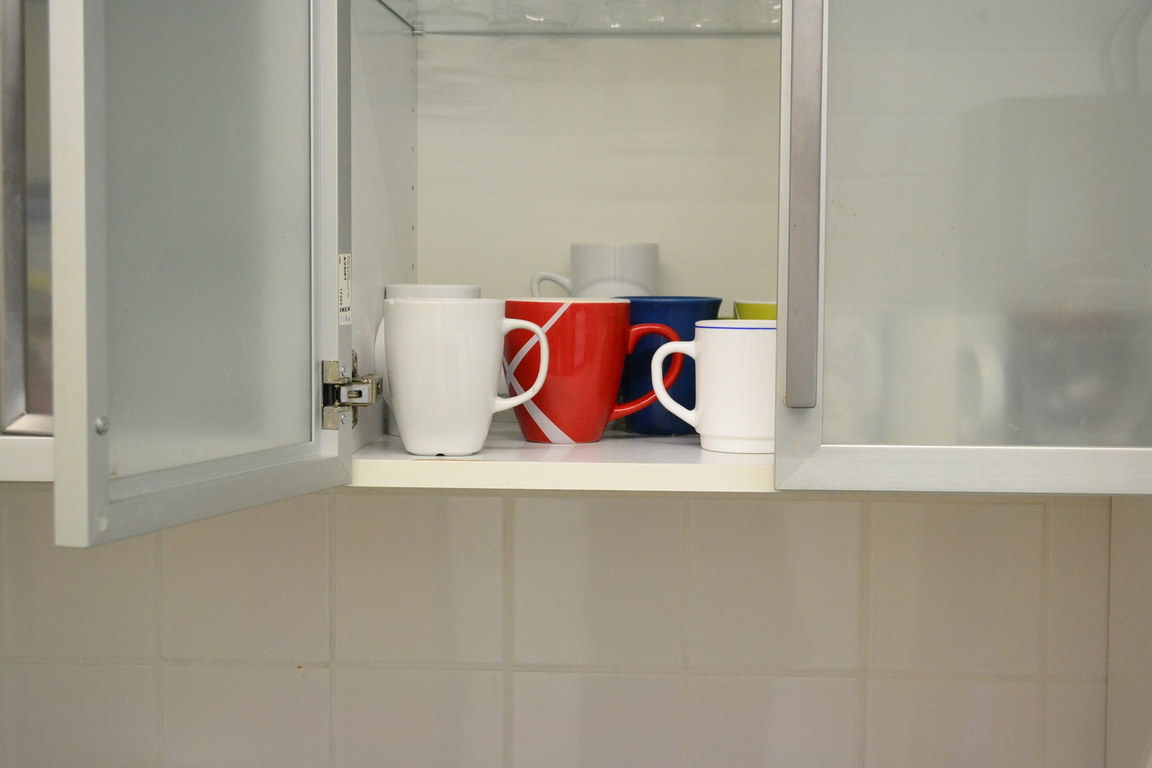
\includegraphics[width=\textwidth]{images/cup_cupboard.jpg}
        \caption{}
        \label{fig:cup-cupboard-basics}
    \end{subfigure}
    ~ %add desired spacing between images, e. g. ~, \quad, \qquad, \hfill etc. 
      % (or a blank line to force the subfigure onto a new line)
      \qquad
    \begin{subfigure}[b]{0.4\textwidth}
        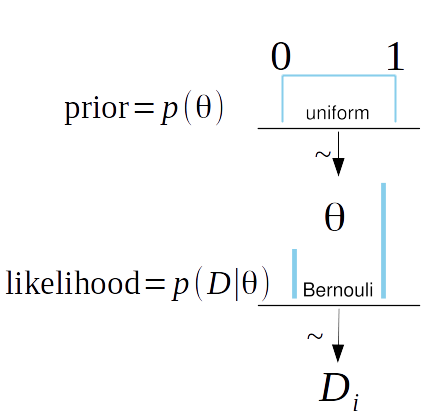
\includegraphics[width=\textwidth]{images/Beta-Bernoulli.png}
        \caption{}
        \label{fig:prior-likelihood}
    \end{subfigure}
\caption[Bayesian learning example]{Bayesian parameter estimation example }
\label{fig: bayes-example}
\end{figure}
We can explain this with an example \cite{lee2014bayesian}. Assume the robot scans a location kitchen cupboard for 10 days at 10:00 am and records if it finds a cup. What we want to estimate is the users preference in keeping a cup in the cupboard in the morning. We define this as $\theta$, which is the possibility of the user keeping the cup in the cupboard. The robot cannot observe the users preference $\theta$. All that it can observe is if the cup is present. First the robot starts by specifying the prior uncertainty with respect to the users preference $\theta$. This uncertainty needs to be expressed as a probability distribution, called the ``prior distribution". In this case,  $\theta$ can range from 0 to 1 then a reasonable ``prior distribution,” denoted by $p (\theta)$, is one that assigns equal probability to every value of $\theta$. This uniform distribution is shown by the dotted horizontal line in Figure \ref{fig: bayes}.


\begin{figure}[htp]
\centering

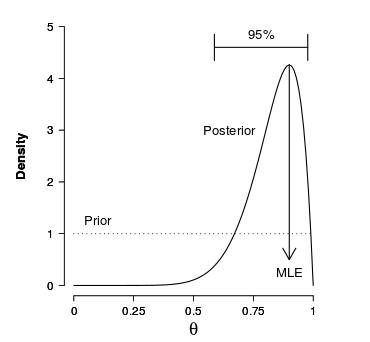
\includegraphics[width=0.5\textwidth]{images/bayes.png}
\caption[Bayesian parameter estimation]{Bayesian parameter estimation for rate parameter $\theta$
, after observing that the cup was present in the cupboard 9 out of 10 days. The mode of the posterior distribution for $\theta$ is 0.9, equal to the maximum likelihood estimate  (MLE), and the 95\% credible interval extends from 0.59 to 0.98 \citep{lee2014bayesian}}
\label{fig: bayes}
\end{figure}

Now we consider the observations made by the robot, and find that the cup was present 9 out of 10 days. After observing the data, the updated knowledge about $\theta$ is described by a \emph{posterior distribution}, denoted by $p (\theta | D)$. This distribution expresses the uncertainty about the value of $\theta$, quantifying the relative probability that each possible value is true value. Bayes rule specifies how we can combine the information from the data, that is how to determine the posterior distribution $p  (\theta | D)$ using  the prior distribution $p (\theta)$ and the likelihood  $p  (D | \theta)$ :
\begin{equation}
	p (\theta | D) = \frac{p (D | \theta) p (\theta)}{p (D)}
\end{equation}

The equation is often verbalized as :
\begin{equation}
	posterior = \frac{likelihood * prior}{marginal\ likelihood}
\end{equation}

We note here that the posterior distribution is a combination of the prior information we had and what we have learned from the data. 




The solid line in Figure ~\ref{fig: bayes} shows the posterior distribution for $\theta$, obtained when the uniform prior is updated with the data. For the posterior distribution in Figure ~\ref{fig: bayes} , a 95\% Bayesian credible interval for $\theta$ extends from 0.59 to 0.98.


\section{Probability Distributions }

The basic idea of Bayesian analysis is that quantification of the \emph{state of belief} or the \emph{state of uncertainty}, about the variables of interest. These variable (latent and observed) are always represented by probability distributions. Probability distribution is just another name for a probability measure. In this thesis we exhaustively use the Beta, Dirichlet, Categorical and Bernoulli distributions. 
 

\subsection*{Bernoulli Distribution}

Bernoulli distribution is used when there are a number of iterations of some activity, where each iteration  (or observation) may turn out to be a ``success" or a ``failure". A Bernoulli distribution takes a single parameter $\theta$, which describes the probability of ``success".  The shorthand $X \sim {\rm Bernoulli} (\theta)$ is used to indicate that the random variable~$X$ has the Bernoulli distribution with parameter~$\theta$, where $0 < \theta < 1$.

A Bernoulli random variable~$X$ with success probability $\theta$ has
probability mass function 
$$
p (x | \theta) = \theta ^ {x}  (1 - \theta) ^ {1 - x} \qquad \qquad x = 0, 1
$$
for $0 < \theta < 1$. Figure~\ref{fig:bernoulli_sample} shows 3 Bernoulli distributions with different values of $\theta$.
\begin{figure}[htp]
\centering
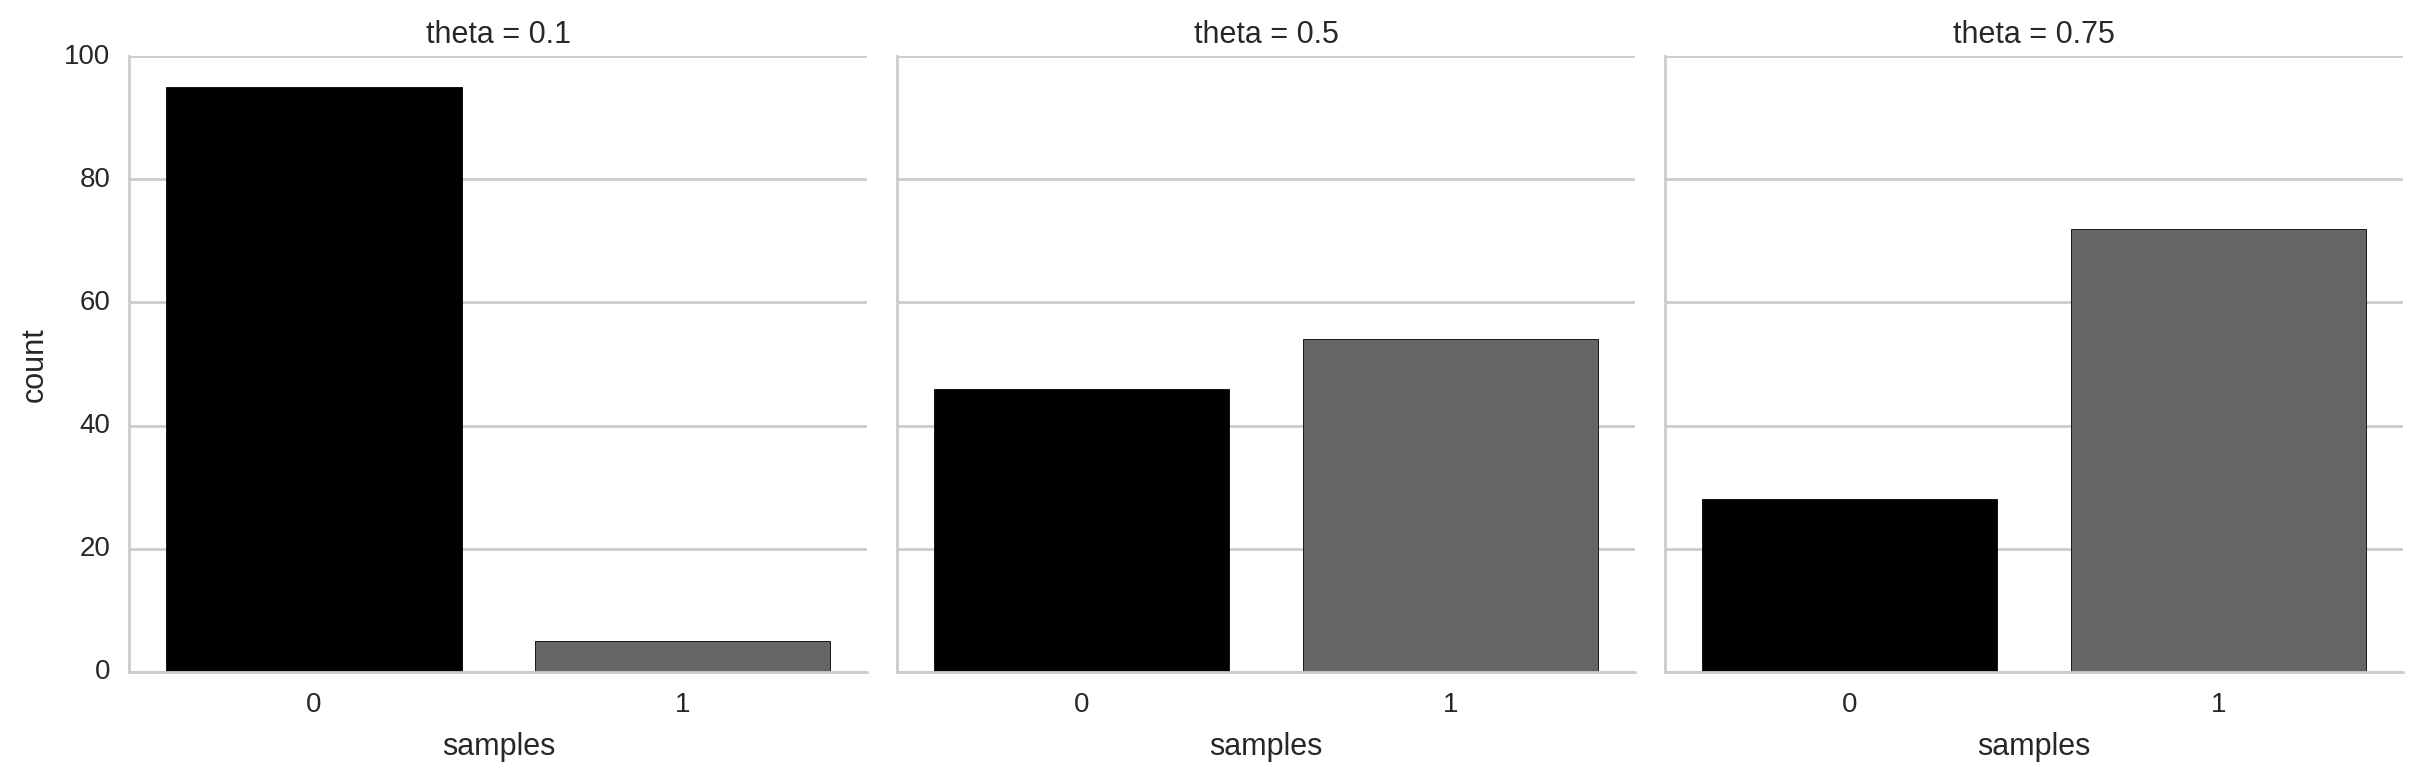
\includegraphics[width=\textwidth]{images/Bernoulli.png}
\caption{Bernoulli Distribution}
\label{fig:bernoulli_sample}
\end{figure}




\subsection*{Categorical distribution}
Categorical distribution is the generalization of the Bernoulli distribution , with more than 2 outcomes.  Categorical takes a parameter $\theta$, which has length k. The probability mass function is :

$$
\prod_{i=1}^k \theta_i^{x_i}
$$

where $\theta_i$ represents the probability of seeing element $i$ and $\sum_{i}p_i = 1$. This is the formulation adopted by \cite{bishop2007pattern}.  Figure~\ref{fig:Categorical_sample} shows 3 Categorical distributions with different values of $\theta$.

\begin{figure}[htp]
\centering
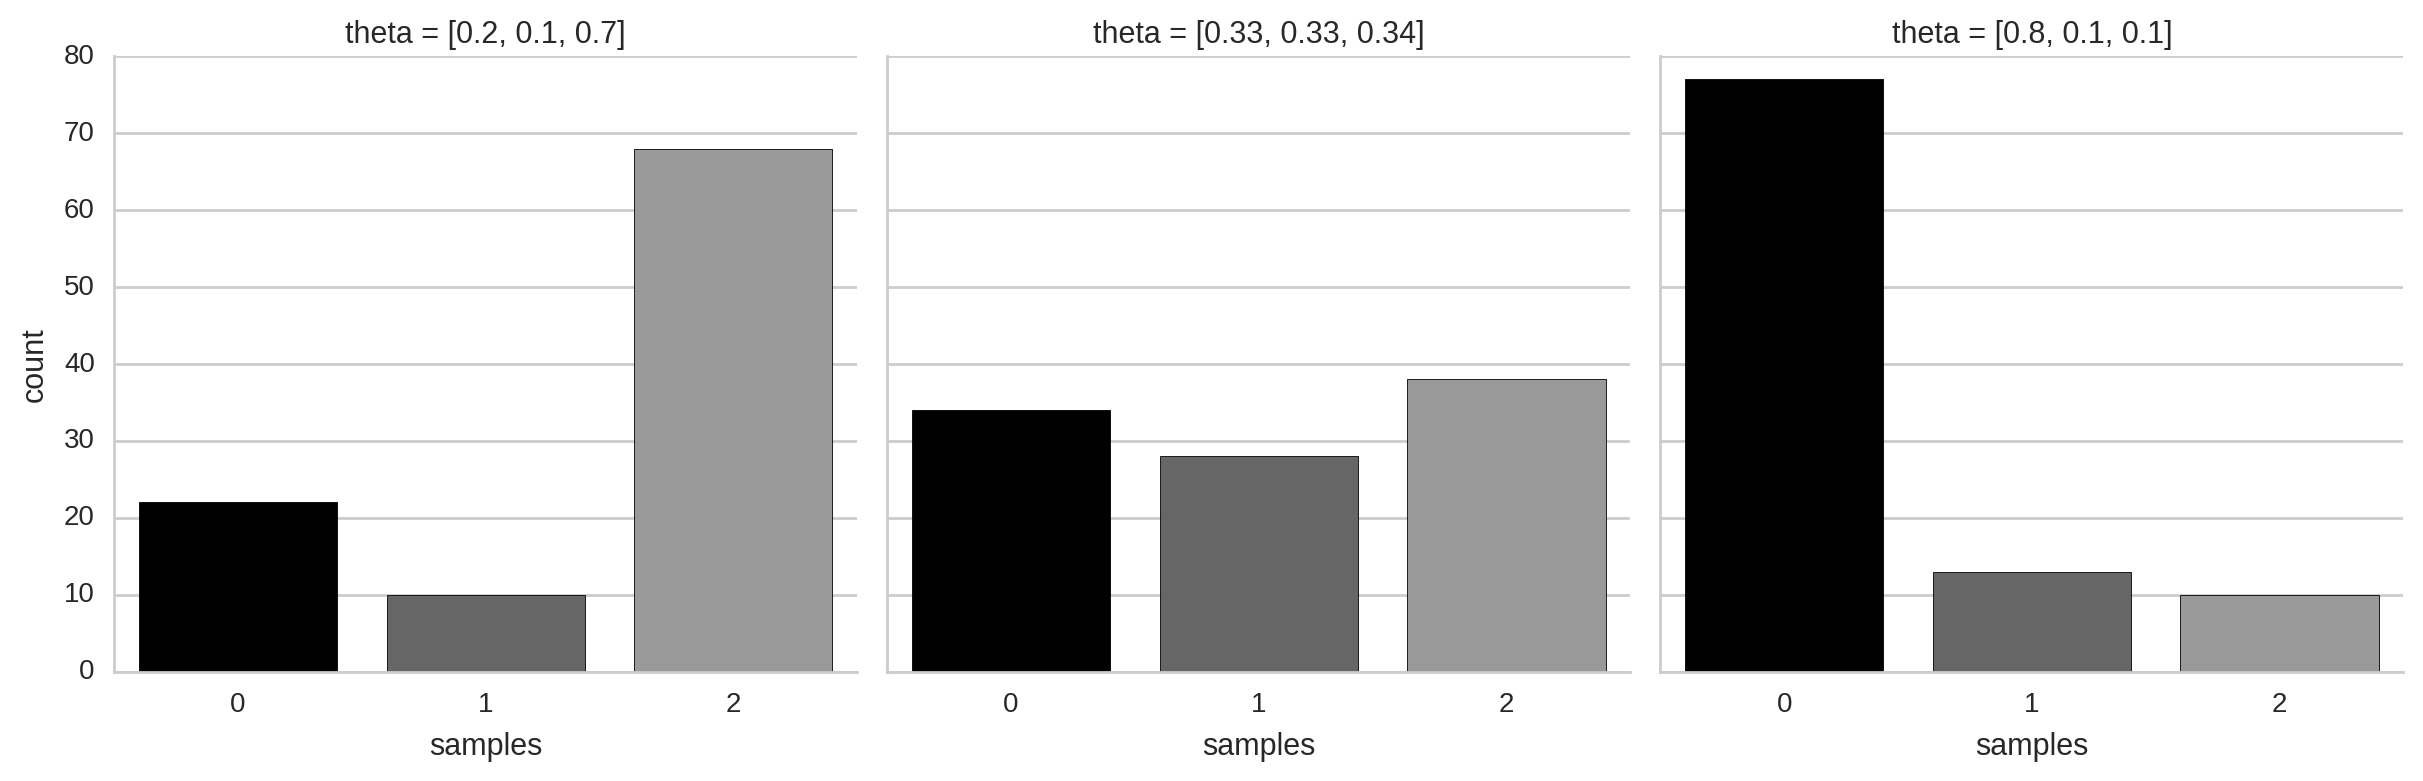
\includegraphics[width=\textwidth]{images/Categorical.png}
\caption{Categorical Distribution}
\label{fig:Categorical_sample}
\end{figure}


\subsection*{Conjugate Distribution}
The term conjugate distribution \cite{BS:BS3830070108} refers to cases where the posterior distribution is in the same family as the prior distribution. In Bayesian probability theory, if the posterior distributions $p(\theta | x)$ are in the same family as the prior distributions $p(\theta)$, then the prior and posterior are called conjugate distributions, and the prior is called a conjugate prior.  Conjugate prior are useful in determining the latent variable of a random variable in graphical model. 


\subsection*{Beta distribution}
The beta distribution beta ( a, b) is a two-parameter distribution with range [0 , 1] and probability distribution function represented as,

\begin{equation}
	p(\theta | a,b) = \frac{ (a + b - 1)! }{ (a -1 )! (b - 1)!}\theta^{a -1}  (1 - \theta)^{b - 1}
\end{equation}

Beta distribution is conjugate prior of Bernoulli and Binomial distributions. Figure~\ref{fig:beta} show Beta distribution with different $a,b$ values.

\begin{figure}[htp]
\centering
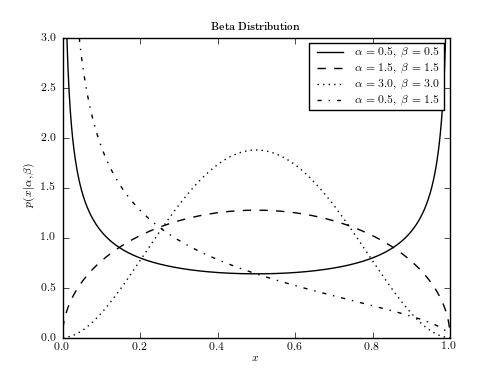
\includegraphics[width=0.5\textwidth]{images/fig_beta_distribution_1.png}
\caption{Beta distribution. \cite{astroMLText}}
\label{fig:beta}
\end{figure}



\subsection*{Dirichlet distribution}
The Dirichlet distribution is part of the exponential family. It has finite dimensional sufficient statistics. It is conjugate to the multinomial and categorical distribution. 


\begin{align*}
    P (\theta | \alpha) &= \frac{\Gamma (\sum_{k=1}^K \alpha_k)}{\prod_{k=1}^K \Gamma (\alpha_k)}\prod_{k=1}^K \theta_k^{\alpha_k-1} \\
			  &= \frac{1}{Z} \prod_{k=1}^K \theta_k^{\alpha_k-1}
\end{align*}

$\alpha$ is a vector with the same size as $\theta$, and it is known as a ``hyperparameter''.  The choice of $\alpha$ determines the shape of $\theta$'s distribution, which you can see by varying it.  If $\alpha$ is simply a vector of ones, we just get a uniform distribution; all $\theta$s are equally probable.

The below table summarizes which distribution to use and what are their conjugate priors.

\begin{tabular}[htp]{|c|c|c|}
\hline
	\textbf{Observations data type} & \textbf{Distribution} & \textbf{Conjugate prior} \\
\hline
\hline
	Boolean & Bernoulli & Beta \\
\hline
	Ordinal & Binomial & Beta \\
\hline
	Nominal & Categorical , Multinomial & Dirihclet \\
\hline

\end{tabular}


\section{Probabilistic Graphical Models}

Probabilistic Graphical Models  (PGM) is the formal lingua franca for probabilistic Bayesian modelling \cite{Tenenbaum2008PP}. PGM is a method to visualize complete and interpretable representation of a Bayesian probabilistic model. The nodes in the graph represent variables of the problem, and the edges connecting them represent dependencies. The graph structure is used to indicate dependencies between the variables, with children depending on their parents. 
The boxes in the graph indicate replication of the variable. The boxes are called as plates. The number inside the plate represent the number of times the variable is replicated. We use the conventions of representing unobserved variables without shading and observed variables with shading.

The model definition and graphical model are depicted in Figure ~\ref{fig:pgm}. Beta distribution with parameters  (1,1), can be selected as the prior distribution, while the ability can be represented using Bernoulli distribution. 
 The observed variable is $D$, represented as a shaded circle. It is dependent on the latent variable $\theta$ represented by a non-shaded circle. The relation between them denoted by the arrow. As there are 10 observations, we draw the plate notation and signify the repetitions.

\noindent
\begin{figure}[htp]

\begin{minipage}{0.3\textwidth}
\centering
\tikz {
\centering
 % Define nodes
  \node[latent]                                  (theta) {$\theta$};
  \node[obs, below=of theta]                     (D)     {$D$}; 
  % Connect the nodes
  \edge {theta} {D};
  % plates
  \plate {location} { (D)} {n=0,....,9};
}
\end{minipage}%
\begin{minipage}{0.7\textwidth}
\begin{equation*}
	\theta \sim Beta (1,1) 
\end{equation*}
\begin{equation*}
	P (D|\theta) \sim Bernoulli (\theta)
\end{equation*}
\end{minipage}
\caption[Graphical Model]{Graphical Model: Shaded node observed variable and non-shaded node is latent variable}
\label{fig:pgm}
\end{figure}

\section{Probabilistic Programming Languages}

Probabilistic programming languages (PPL) are new languages developed to program probabilistic graphical models and to run inference in them. The development of Markov chain Monte Carlo  (MCMC) algorithms and software, combined with fast computer hardware were the main factors behind the current rapid adoption of Bayesian data analysis to real-world applications \citep{kruschke2014doing}. Probabilistic programming is a new approach using which one can construct Bayesian models faster using compact code and in a less error-prone way \citep{dippl, luttinen_bayespy_2014}. 


\begin{figure}[htp]
\centering
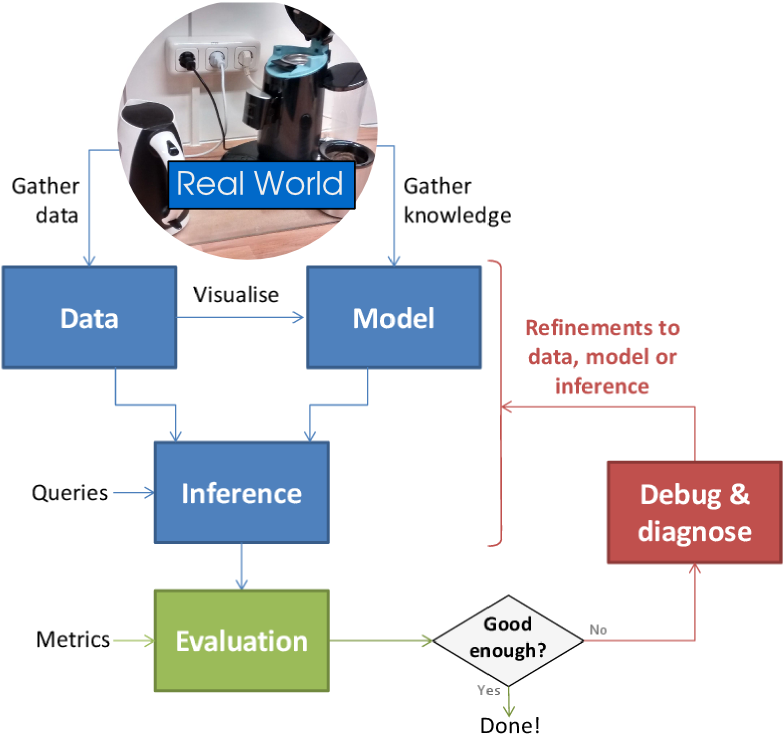
\includegraphics[width=0.5\textwidth]{pictures/Lifecycle.png}
\caption[Steps involved in probabilistic modelling ]{Steps involved in probabilistic modelling  \cite{winn2016} }
\label{}
\end{figure}


\textbf{Probabilistic Programming  (PP)} gives us a framework in which we can create any Bayesian model, based on our assumptions of the process \cite{winn2016}. The model is basically expressing the assumptions in a mathematical form. The assumptions are the number of variables in the model, the relation between these variables, changes in which variables affects which other variables. This model is then used to generate a problem specific algorithm which can be used to solve the machine learning problem in hand. 

\subsection*{Steps required in Probabilistic Modelling \cite{winn2016}}
\label{sub:steps}
\begin{enumerate}
	\item \textbf{Gather data} to be used for training and evaluation.
    \item \textbf{Gather knowledge} required for model building.
    \item \textbf{Visualise} the data to understand it. This is useful also for gathering knowledge. After visualisation the insight gained can be used for assumptions in model building.
    \item \textbf{Construct a model} based on the knowledge of the problem statement available and data visualisation. 
    \item \textbf{Perform inference} using both the data and the constructed model. The variables of the model are tuned based on the data available. Predictions can be made to find out the knowledge gained by the model.
    \item \textbf{Evaluate} the performance of the model based on evaluation metric.
    \item \textbf{Diagnose} the model and the assumptions if the evaluation is below some acceptable range
    \item \textbf{Refine the system} by adapting different model structure and inference engine

\end{enumerate}
% subsection steps  (end)

Examples of Probabilistic programming languages include CHURCH \cite{goodman_church_2012}, Anglican \cite{wood2014new},  Venture \cite{mansinghka_venture_2014}, PyMC3 \cite{salvatier_probabilistic_2015}, BayesPy \cite{luttinen_bayespy_2014} and Infer.net \cite{minka_2010}. There are many other languages currently in development, and probabilistic programming has become a very active field of research.

\subsection{PyMC3}

\textbf{PyMC3} is python module for Bayesian modelling. It provides intuitive model specification syntax for designing the models. The inference is primarily focussed on advanced MCMC fitting algorithms.


\subsection{BayesPy}

\textbf{BayesPy} provides tools to do Bayesian modelling. In BayesPy users construct their models, observes data and then runs inference. The inference engine present in BayesPy is variational Bayesian inference.

Below we show example code of the Beta Bernoulli model depicted in Figure~\ref{fig:pgm}, implemented in Bayespy and PyMC3.

\noindent\begin{minipage}{.46\textwidth}
\begin{lstlisting}[caption=BayesPy Code,frame=tlrb]{Name}
import bayespy as bp

observations = [1, 1, 1, 1, 0, 1, 1, 1, 1, 1]


theta = bp.Beta ([1, 1])
D = bp.Bernoulli (theta, plates= (10,))
D.observe (observations)
theta.update ()

\end{lstlisting}
\end{minipage}\hfill
\begin{minipage}{.46\textwidth}
\begin{lstlisting}[caption=PyMC3 code,frame=tlrb]{Name}
import pymc3 as pm

observations = [1, 1, 1, 1, 0, 1, 1, 1, 1, 1]

with pm.Model () as model:
    theta = pm.Beta (1, 1)
    D = pm.Bernoulli (observed=observations)
    step = pm.NUTS () 
    trace = pm.sample (100, step)
    
\end{lstlisting}

\end{minipage}


Thus the same graphical model is implemented in two different languages. The user doesn't need to worry about the underlying distribution implementations and work directly at the model level. This makes modelling easy and less error-prone. 


\section{Fawkes}
Fawkes is a robot software framework developed at the Knowledge based Systems Group  (KBSG) at RWTH Aachen University \citep{niemueller2010design}. It is a component-based Software Framework. It can be used for various robotics real-time applications and domains. It can run on multiple platforms. Functionalities in Fawkes are implemented as \emph{plugins}. Fawkes is designed to support fast information exchange  between different plugins via \emph{Blackboard}. In this thesis, we are interested in the \emph{mongodb-log} \footnote{\url{https://www.fawkesrobotics.org/projects/mongodb-log/}} plugin \citep{niemueller2012generic}. The mongodb-log plugin when loaded records all data stored in the blackboard  and all images and point clouds available to the specified MongoDB\footnote{\url{https://www.mongodb.com/}} database. 

\chapter{Approach}
\label{cha:approach}

The central idea of the thesis is based on the assumption that humans do their activities in the context of time. Humans follow a certain routine in their lifestyles and time is one de-facto latent element in determination of these routines. Most of the activities in ones daily life can be associated with the time of the day. Thus time is a prominent factor while learning human behaviours and preferences. All the models developed in this thesis try to learn human behaviours and preferences based on time as factor. 

\section{Problem Formulation}
In this thesis we use Bayesian models for representing the learned knowledge about human behaviour and preferences. We formulate the problem as getting an accurate probability density of possible locations given the previous observed locations. Given the corresponding observations of $D_{o_i}$, the probability distribution over the locations of $o_i$ at time $T$ is governed by the following formula 

    \begin{equation} \label{eq:1}
	    P(l_i | t_i, D_{o_i})
    \end{equation}

   Various temporal information related to periodic patterns can be implied by $T$, to indicate the location distribution. Such as specific hours of the day (11:00 pm), a day of the week(Friday), or a month of the year(February). We use the \textbf{temporal state} to represent such information and introduce $r(t)$ to denote temporal state extracted from time $T$,.  Dependency on the type of the temporal state $r(t)$ can be a different function. For example,if $r(t)$ denotes temporal state in terms of hours of the day then $r(t) \in {0,1 ... , 23}$, if $r(t)$ denotes temporal state in terms of day of the week, then $r(t) \in {0,1, .. 6}$ . Without loss of generality, we use $r(t)$ to denote a type of temporal state in the following description, Equation \ref{eq:1} is reformulated as 
    
    \begin{equation}
	    P( l_i | r(t), D_{o_i})
    \end{equation}
    
    Applying Bayes Rule
    
    \begin{equation}\label{eq:3}
	P( l_i | r(t), D_{o_i}) \propto P(r(t) | l_i, D_{o_i})  P(l_i | D_{o_i})
    \end{equation}
    Where:
    \begin{itemize}[label=]
    \item $P(r(t) | l_i, D_{o_i})$ : Temporal context 
    \item $P(l_i | D_{o_i})$ : Spatial context
    \end{itemize}
    
     The spatial context $P(l_i | D_{o_i})$ indicates the location distribution of object or person $o_i$ given the previous observed location $D_{o_i}$ . The temporal context $P(r(t) | l_i, D_{o_i})$ represents the temporal state distribution of object $o_i$, being observed at location $l_i$ with corresponding $D_{o_i}$
    


\begin{tabular}{cp{8cm}}
    \hline
	Symbol & Meaning\\
	\hline
	O & Set of all objects or persons\\
	$o_i$ & Single object from the set $O$, $o_i \in O$ \\
	$L$ & Set of all locations\\
	$l_i$ & Single location from the set $L$. $l_i\in L$\\
    $T$ & Time interval\\
    \hline
	$<o_i,l_i,t_i>$ & object $o_i$ was located at location $l_i$ at time $t_i$\\
	$D$ & Collection of all objects all observed locations\\
	$D_{o_i}$ & Previous observed locations of $o_i$\\ 
    \hline
     $P(r(t) | l_i, D_{o_i})$ &  Temporal context representing the temporal state distribution of $o_i$ at location $l_i$ given previous observations $D_i$\\
     $P(l_i | D_{o_i})$ & Spatial context representing the location distribution of object $o_i$ given the previous observations $D_{o_i}$\\
    \hline
\end{tabular}
% section Problem formulati (end)

\section{Model Implementation}

In this thesis, we use probabilistic approach to knowledge acquisitions, which models learning and reasoning as inference in complex probabilistic models. In particular, we examine how robots can quantitatively  develop knowledge from information,  modelled using  functional probabilistic programming languages. 


\section{DIKW pyramid}
\todo[inline]{TODD}

\section{Architecture}
\todo[inline]{TODO
Robot uses records it sensors values ,
Robot uses the sensors readings and converts to information ,
the information is stored in robot memory. 
On regular basis or on trigger the the knowledge generation software is trigger which generates the knowledge and adds back to the robot memory 

}
\label{cha:}
\begin{figure}[htp]
\centering
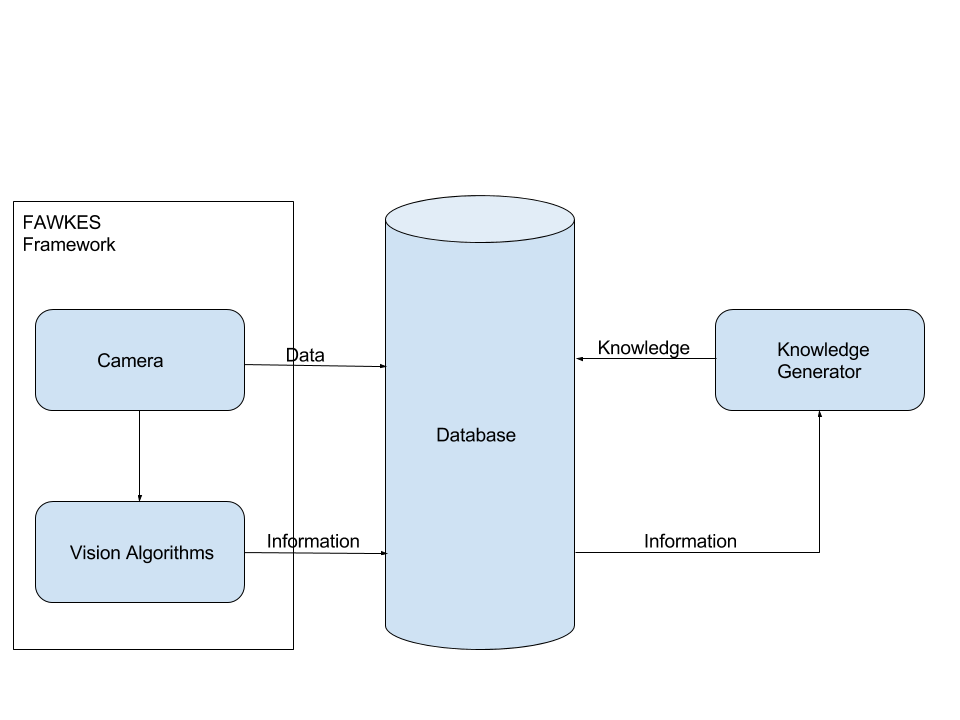
\includegraphics[width=\textwidth]{images/integration.png}
\caption{Integration with the robot memory}
\label{}
\end{figure}


\section{Notation and terminology}
Throughout the thesis, we are referring to entities such as ``locations," ``hours," and ``observations".
This helps to guide intuition and maintain continuity of thoughts as we guide through related problems involving collections of data.
Formally we define the following terms:
\begin{itemize}
	\item A \emph{location} is the basic unit of the discrete data, defined to be an item from a set of locations. These locations can be rooms of the home or different compartments of the kitchen. 
	\item An \emph{period} is a sequence of $N$ locations denoted by $\textbf{p} = {x_1;x_2;:::;x_N}$. These represents the locations observed in a particular period of time.
	\item A \emph{observations} is a collection of $T$ periods denoted by $ D = {p_1;p_2;:::;p_T}$. These represents the complete data collected by the robot.
\end{itemize}


We also use the entities such as ``data," ``information," and ``knowledge" throughout the thesis. These can be define as:
\begin{itemize}
	\item A \emph{data} corresponds to sensor output. All the output of the sensors recorded by the robot is a data. For example RGB image from a camera, depth points from depth sensors etc.
	\item A \emph{information} corresponds to output of algorithms which process on the above data. For example vision algorithms process RGB images data to extract information of objects or persons in the image.
	\item A \emph{knowledge} corresponds to output of algorithms which process on the above information. For example vision algorithms can process detected object information in consecutive RGB frames to extract knowledge that the object was moving.
\end{itemize}

% section  Things to study (end)
\chapter{Learning User Preferences In Object Placement}
\label{chapter: object}

As robots achieve long term autonomy and they intend to stay longer in human environments, they should be ability to adapt quickly to the corresponding environments especially to the humans within. As a robot makes new observations, it should attempt to use these observations to learn about the user preferences. In this chapter we discuss on problem to enable a robot to learn about user preferences in object placement in a specific home. 

In a series of interviews to understand the needs of people with robots, \cite{pantofaru_exploring_2012} concludes that one of the
expectations from robots is help in organizing things based on the user preferences. Since they are service robots it is acceptable for a new robot to ask for help from its user in the initial days it moves to a new home. But as the robot stays longer in a home it becomes less acceptable that the robot asks the same questions, i.e. they should have the capabilities to learn from previous information provided by the user. The Robots should also be able to reason and learn from its own observations of the user and the environment. It should have mechanisms to generate new knowledge about the user and environment from all information gathered. For example, the robot can learn about the user preferences of the cutlery used to setup a breakfast table from observations of breakfast tables in the past. In this chapter we look at such one example of knowledge generation based on previous observations, for learning the user preferences in object placement.

The advantage of learning user preference about object placement would be in object search. In classical object search, the search is improved based on the knowledge of object locations in a generic home  (for example, cups are found in kitchen, books in shelves) by \cite{samadi_using_2012, joho_learning_2011}. The above method is good for a new robot but after long time stay, the robot needs to adapt its beliefs for searching based on its user's preferences. Another use of the user preferences will be in organizing the home. Here the robot should learn  about the default locations of different objects, so that the robot can return any misplaced objects back to their locations. Understanding user preferences in organizing objects in a home has 
been studied by  \cite{abdo2015robot}, where robots learn based on the data collected via crowd-sourcing.  From practical experience we know that even though homes have same base structure in space, the usage of space is based on the user preferences. Each home is different from any other home because the humans which reside in them use it according to their likes  (for example, some users the keep books on the study table and not on shelves). The proposed methods in this chapter will try to enable the robot learn these user preferences specific to each home. So rather than the robot learning object locations in a generic home the proposed methods shall learn object locations in a specific home.


\begin{figure}[htp]
\centering
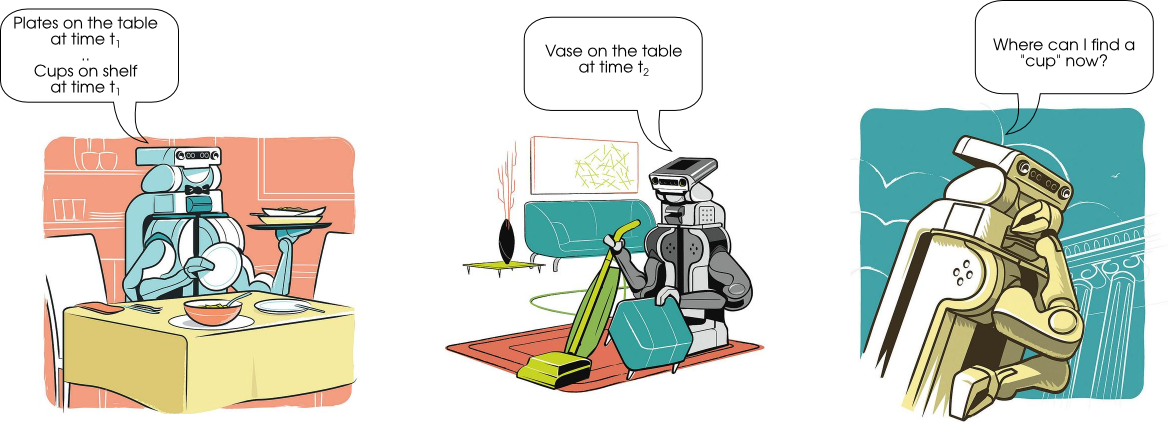
\includegraphics[scale=0.4]{pictures/scenario.png}
\caption[Example scenario of robot recording objects location and time]{Robot recording objects location and time. Based on the
recordings robot making prediction on the location of the cup for current time
Images courtesy : \citep{willowgarage} }
\label{scenario}
\end{figure}

Autonomous robots in dynamic human environments convert raw data  (e.g. image) to information  (e.g. cup on table) for completing their tasks. This information can be used by the robot to generate knowledge about user preferences. We explain this in the context of the ``make coffee" example introduced in the Chapter~\ref{chapter:Introduction}. 
Consider a domestic robot, which has been placed in a home environment with a known map and semantic information of the different locations in the home. The domestic robot while doing its daily activities over the course of weeks or months, makes records. Now the robot has been asked to bring the coffee mug of the user.
The robot has to decide which part of the home it has to go to look for
the coffee mug. The robot can make this decision based on the previous observations of locations of the coffee mug.
The robot, using these previous observations and the time of those observations,
makes a prediction about where the coffee mug can be found at the current time.
Based on previous observation it can be inferred that the coffee mug is usually found in any of the following three locations: dishwasher,counter or cupboard. Assuming that the time now is morning, from previous observations it can be found that the coffee mug was always found  in the dishwasher. The above example illustrates the main aspects of object location prediction we wish to capture in this chapter.

\section{Approach}

We formulate the problem of learning user preference in object placement, by modelling the belief of \emph{finding an object at a location}. The robot tries to learn the chances of the user of keeping an object  (e.g. cup ) at a location  (e.g. cupboard). Whenever the robot scans a particular location as illustrated in Figure~\ref{fig:counter_scan}, it records present and absent of objects at that location along-with the time of the scan ~\ref{tab:robot_record}.
  
  
  \begin{minipage}{\textwidth}
  \begin{minipage}[b]{0.49\textwidth}
    \centering
        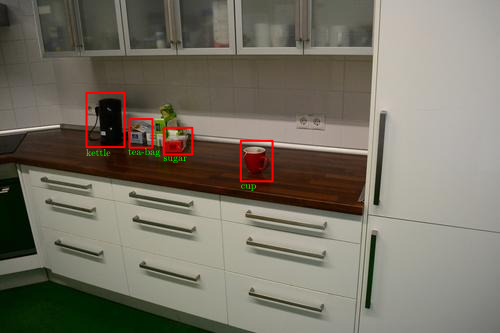
\includegraphics[width=0.9\textwidth]{images/counter_ano.png}

    \captionof{figure}{Robot scanning kitchen counter}
    \label{fig:counter_scan}
  \end{minipage}
  \hfill
  \begin{minipage}[b]{0.49\textwidth}
    \centering
    \begin{tabular}{|l|l|l|l|}
        \hline
	        Time & Location & Object & Present\\
        \hline
        \hline
	        09.03 & counter & kettle & True\\
        \hline
	        09.03 & counter & tea-bag & True\\
        \hline
	        09.03 & counter & sugar & True\\
        \hline
	        09.03 & counter & cup & True\\
        \hline
	        09.03 & counter & plate & False\\
        \hline
	        09.03 & counter & milk & False\\
        \hline
        \end{tabular}
      \captionof{table}{Robot record}
      \label{tab:robot_record}
    \end{minipage}
  \end{minipage}



This recorded information about each object at each location is modelled using Bayesian models to learn about the belief of a person placing an object at any location.

The observations made by the robot are boolean values (present or absent). As discussed in chapter~\ref{chapter:basics}, when the data type is boolean we can use the Bernoulli Distribution with a Beta distribution prior to model the observations. To capture the belief at different times of the day, we create 24 Bernoulli variables, one for each hour. For coping with the problem of sparsity of observations in all time periods, we also add a hyper-prior. The addition of the hyper-prior causes of sharing of learning knowledge in one time period with other time periods. The model is called as the \textbf{Hierarchical Beta Bernoulli}(HBB)  model. In the next section we explain the generative model along with the graphical diagram. 


\section{Hierarchical Beta Bernoulli Model}

Hierarchical Beta Bernoulli model is a three-level Bayesian model. The basic idea is that observations of the presence of an object at a location (first level), is characterized by a distribution for each hour (second level), which share information via a common latent distribution (third level).

The data are the boolean observation of the object at a location $x_{ij}$ for $i = 1 \dots T$ time periods and then $j = 1, \dots , N$  are the observations.  We assume that the latent pattern that the user will place the object at a  location in a particular period can be represented as a Bernoulli distribution. The number of periods $T$ for our model is fixed to 24 corresponding to the number of hours in a day. 

The conjugate prior for the Bernoulli distribution is the Beta distribution. The model estimates the posterior distribution of $\theta_i$ given our current data and prior beliefs. Our prior beliefs are encoded in the model through the prior $\alpha$ and $\beta$, which represents pseudocounts of what we believe the data should look like – currently taken as same values representing no prior information. The probabilistic graphical model is shown in Figure \ref{bbm}

\noindent
\begin{figure}[htp]

\begin{minipage}{0.3\textwidth}
\centering

\tikz {
 % Define nodes
  \node[latent]                                  (theta) {$\theta$};
  \node[latent, above=of theta, xshift=-1.2cm]   (alpha) {$\alpha$};
  \node[latent, above=of theta, xshift=1.2cm]    (beta) {$\beta$};
  \node[obs, below=of theta]                     (y)     {$x$}; 
  % Connect the nodes
  \edge {alpha,beta} {theta} ; %
  \edge {theta} {y};
  % plates
  \plate {location} { (y)} {location};
  \plate {time} { (theta) (y) (location)} {time};
}

\end{minipage}%
\begin{minipage}{0.7\textwidth}

\begin{equation*}
	\alpha \sim Beta (2,2) ; \beta \sim Beta (2, 2);
\end{equation*}
\begin{equation*}
	\theta \sim Beta (\alpha, \beta);
\end{equation*}
\begin{equation*}
	x = Bernoulli (\theta)
\end{equation*}
\end{minipage}
\caption[Hierarchical Beta Bernoulli graphical model]{Graphical model representation of Hierarchical Beta Bernoulli model. The boxes are ``plates" representing replicates. The outer plates represents hours of a day, while the inner plate represents whether object was observed at the location each hour.}
\label{bbm}
\end{figure}

The models are implemented using the PyMC3 probabilistic programming language.

\FloatBarrier
\section{Experiments}

We tested our approach on artificially generated datasets as well as on a real dataset of object locations collected by a long term robot.
The goal of the experiments were to
\begin{itemize}
    \item verify that the robot is able to learn the user preference in placing an object at a particular location
	\item empirically conclude on the minimum number of times a location needs to be scanned before a robot can start predicting with 80\% confidence?
	\item evaluate the accuracy of the developed model.
\end{itemize}

\subsection{Evaluation Of Number Of Observations Required}

To quantitatively evaluate the accuracy of the learned model we generated a synthetic dataset of object locations, with known ground truth. The dataset consists of observations, made by a mobile domestic robot, of a cup on the counter during different times of the day. The robot scans the counter-top of the kitchen while doing its daily chores. While doing so it records all the instances that it finds the cup on the counter. Figure \ref{simulation} shows the ground truth probabilities as well as the count of the different observations generated from the ground truth.

\begin{figure}[htp]
\centering
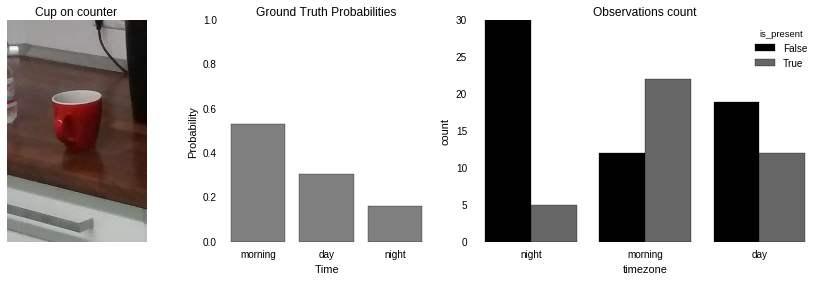
\includegraphics[width=\textwidth]{images/object_simulation.png}
\caption[Simulated object location dataset]{Simulated Object location dataset: Ground truth probabilities of finding a cup on the counter during different times of the day. Observation count of the dataset generated from the ground truth probabilities}
\label{simulation}
\end{figure}

The generated dataset is provided to the HBB model which runs its inference algorithms and updates its posterior probabilities. The performance of the model can be measured by using the distance between the learned probability and the ground truth probability.  The distance between the learned and ground probabilities is measured using the Bhattacharyya distance. The learned models were also validated using cross-validation technique. Each dataset was split into training and testing dataset. The training set was used for learning while the testing set was used for validation. Based on the validation we measure the accuracy score. 


\subsubsection*{Bhattacharyya distance}
We use the Bhattacharyya distance \cite{bhattacharyya1946measure} to quantify the distance between the learned probability and the ground truth. Bhattacharyya distance measures the similarity of two discrete or continuous probability distributions. 
Let  $p$ and $q$ be two discrete probability distributions over the same domain $X$. The Bhattacharyya co-efficient \cite{bhattacharyya1946measure} is a divergence-type measure between distributions, defined as,
\begin{equation}
	BC = \sum_{x\in X}\sqrt{p (x)  q (x)} 
\end{equation}

If $p (\theta_i)$ and $p (\theta_j)$ represent two Bernoulli distributions, then the Bhattacharyya co-efficient is derived as,
\begin{equation}
	BC (p (\theta_i), p (\theta_j)) = \sqrt{p (\theta_i) p (\theta_j)} + \sqrt{p (1- \theta_i) p (1 - \theta_j)}
\end{equation}

When both the probabilities are same $BC = 1$ . The Bhattacharyya distance is then provided by 
\begin{equation}
    D_B = -\log (BC)
\end{equation}

The Bhattacharyya distance ranges from 0 to $\infty$, with \textbf{0} meaning both probabilities are identical. 


\subsubsection*{Accuracy }

The accuracy is the proportion of correct predictions \cite{scikit-learn} . If $p_i$ is the predicted value of the $i_th$ sample and $o_i$ is the corresponding true value, then the fraction of correct predictions over $n_{samples}$ is defined as 

\begin{equation}
	accuracy (p, o) = \frac{1}{n_samples} \sum_{i=0}^{n_{samples} -1 }1 (p_i = o_i)
\end{equation} 

where $ 1 (x)$ is the indicator function.


We evaluated the number of observations required to learn a pattern by comparing the learned models  probabilities with the ground truth per time period. The model is trained with increasing number of observations, and the learned probabilities are compared with the ground truth. For each size of the observations, the procedure is repeated 100 times using different ground truth probabilities.

\subsubsection*{Results}
The Bhattacharyya distance between the posterior probability and the ground truth probability is shown in Figure \ref{fig:object_simulation_distance}. The accuracy of the model using increasing number of training is show in Figure \ref{fig:object_simulation_accuracy}. We can observe from the results that with \textbf{25} observations the mean distance is reduced below 0.01 and the accuracy is above 80\%. Thus we can empirically conclude that a minimum of \textbf{25} observations per location had to be made by the robot to make valid predictions of the object locations. 

\begin{figure}
    \centering
    \begin{subfigure}[b]{0.4\textwidth}
        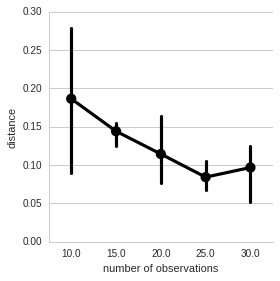
\includegraphics[width=\textwidth]{images/object_simulation_error.png}
        \caption{}
        \label{fig:object_simulation_distance}
    \end{subfigure}
    ~ %add desired spacing between images, e. g. ~, \quad, \qquad, \hfill etc. 
      % (or a blank line to force the subfigure onto a new line)
      \qquad
    \begin{subfigure}[b]{0.4\textwidth}
        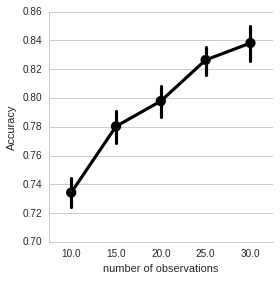
\includegraphics[width=\textwidth]{images/object_simulation_accuracy.png}
        \caption{}
        \label{fig:object_simulation_accuracy}
    \end{subfigure}
    \caption[Evaluation of number of observation required]{Evaluation of number of observation required: Distance between ground truth and learned probabilities (a). The accuracy of the learned models using different number of observations (b) }\label{fig:object_simulation_accuracy}
\end{figure}

\FloatBarrier
\subsection{Evaluation Of Model Accuracy}

In this section we evaluate the accuracy of the model by using a real world dataset. The KTH Object dataset \cite{krajnik_wheres_2015}, was collected in the Computer Vision and Active Perception lab at KTH Stockholm, by a SCITOS-G5 mobile robot over  the  course  of  five  weeks.  The robot conducts two to six autonomous patrols per day, around the lab, visiting three waypoints. On reaching each waypoint the robot would scan the area using a pan-tilt sweep. In each sweep the data from its RGB-D sensor are collected. The KTH dataset contains approximately 100 observations per waypoint. The dynamic objects of the environment were identified  using the `MetaRoom' method by \cite{ambrucs2014meta}. There were 37 different dynamic objects identified by the algorithms. These objects were manually labelled by \cite{krajnik_wheres_2015}.

\begin{figure}[htp]
\centering
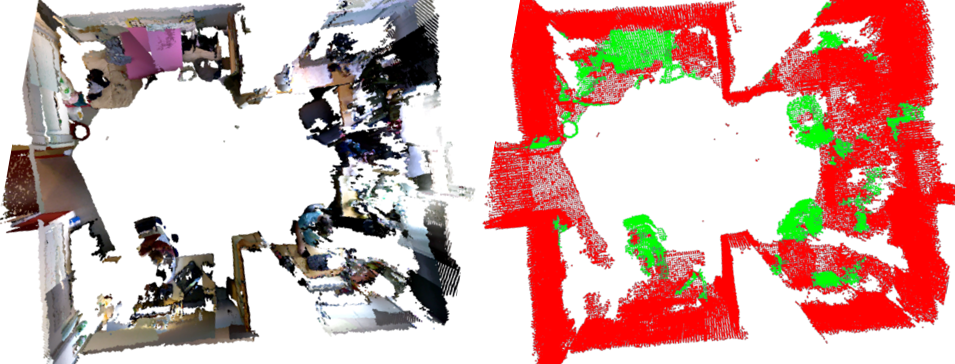
\includegraphics[width=\textwidth]{images/kth-dataset-fromsite.png}
\caption[KTH dataset collection]{KTH dataset collection \cite{krajnik_wheres_2015}. Object retrieval from point cloud data. The points depicted as green denote dynamic objects in the environment}
\label{fig:KTH-dataset}
\end{figure}



\subsubsection*{Results}

The first four weeks of the KTH dataset is used to train the models and the fifth week is used to evaluate the learned model. The accuracy results of 37 objects is plotted in Figure~\ref{fig:kth_object_evaluation} . 
Out of the 37 objects \textbf{26} objects have a accuracy rate of above \textbf{70\%} which is denoted by the dotted line. Most of these 26 objects were static objects like chairs, computers etc. as a result of which they had good accuracy. The model was not able to accurately predict locations of objects that had seemingly random patterns of locations.
\begin{figure}[htp]
\centering
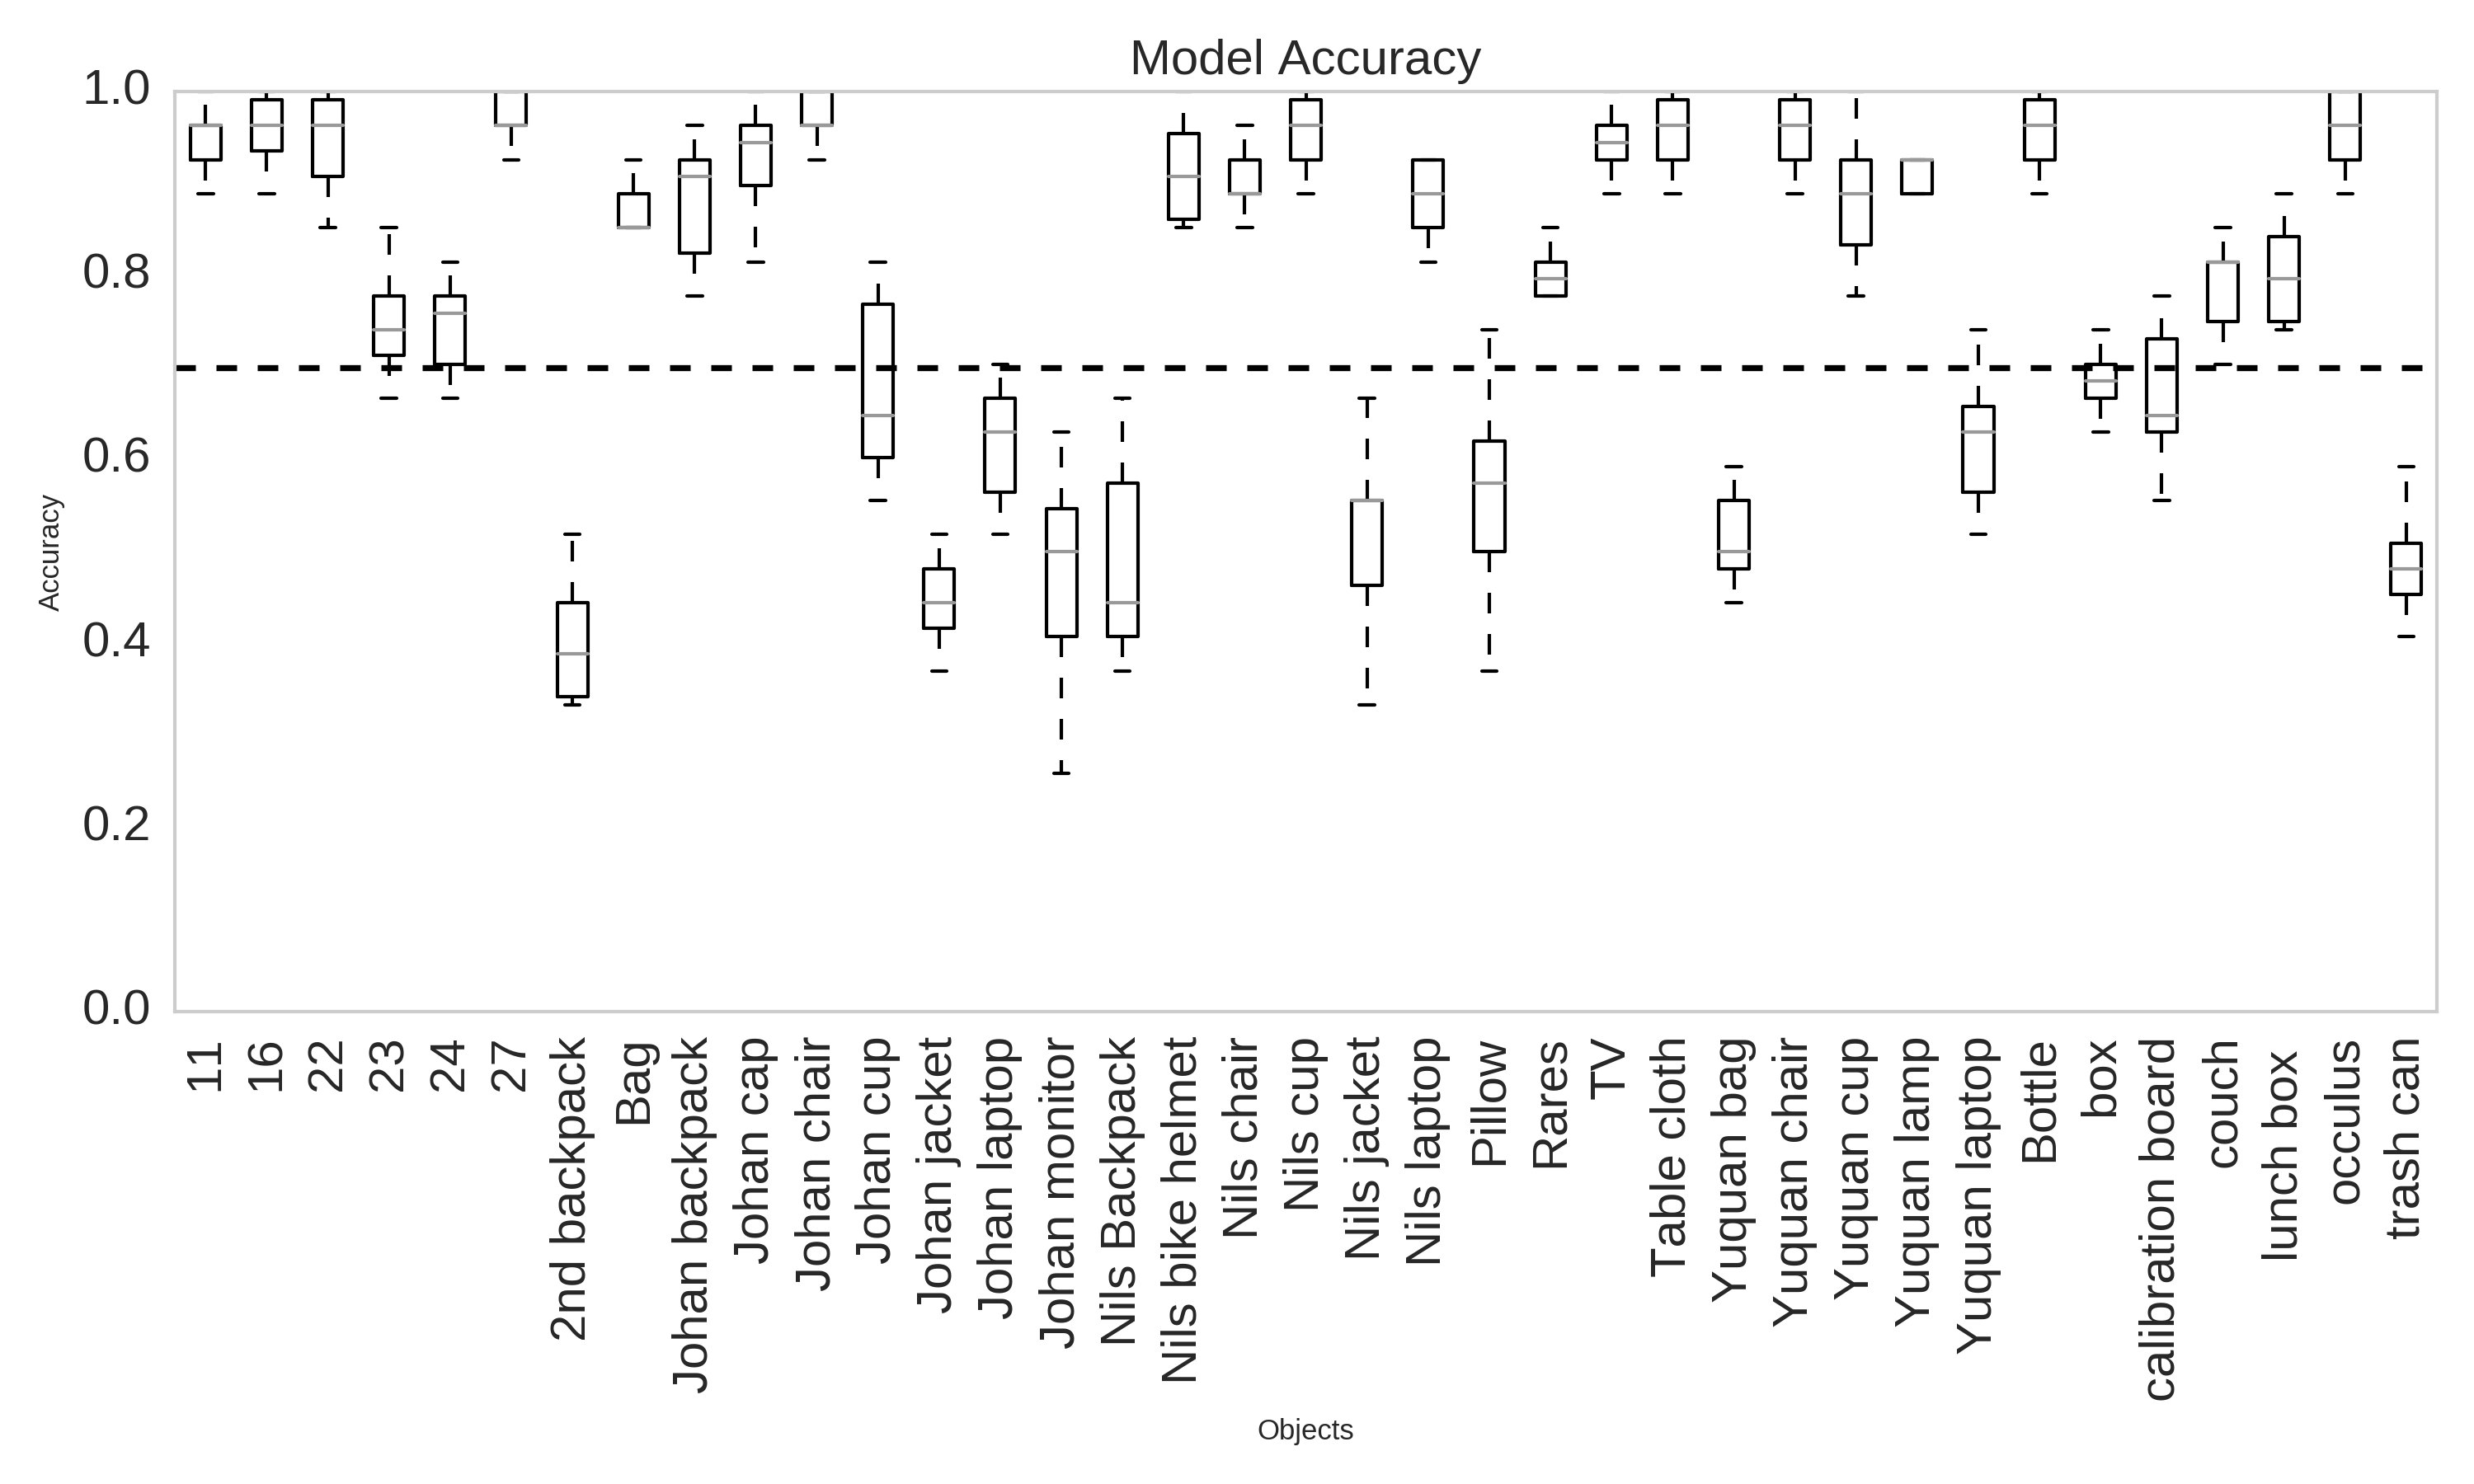
\includegraphics[width=\textwidth]{images/evaluation_kth.png}
\caption[Cross validation results]{Cross validation results. x-axis is the name of the object, y-axis represents the accuracy in predicting the locations of the objects. }
\label{fig:kth_object_evaluation}
\end{figure}

\FloatBarrier
\section{Discussion}
In this chapter, we presented a probabilistic model for learning user preference in placing an object at a particular location. 
Our first contribution is to represent the user preferences of object placement using graphical model. 
Our second contribution is that the graphical model has been implemented using a probabilistic programming language. 
The robot continuously learns about where the user prefers to keep his objects in the home from the set of object location observations. 
Since the observations are not a continuous trace but just random instances of the objects, the model was designed to be able to capture the latent knowledge in the placement preferences from such sporadic observations.

We have shown by evaluation that the robot needs minimum 25 observations per location to make valid prediction about the object being in that location in this dataset. As seen from evaluation objects which are not moved very often are learned very easily by our models using few observations. The model performs badly when there is no preference in the user placement i.e. it seems the user places randomly. 
From the real world experiments we can conclude that a majority of the objects in our home environments are rarely moved by the user, therefore our model is able to learn and predict accurately for most of the objects. 

The approaches here capture knowledge about each object in each location separately, we will see in chapter \ref{chapter:Human location} how knowledge about multiple locations of the object can be captured in a single model.
\chapter{Learning Room Occupancy based on User Routines}
\label{chapter:occupancy}
In this chapter, we investigate how a robot can learn occupancy period of different rooms of a office or home based on user's routine. Occupancy represents the belief of the robot about when are rooms occupied or empty. The probabilistic model developed in the previous chapter enables a domestic service robot to learn the user preference for object placement on each locations. We use the same models in this chapter to learn about the occupancy of each rooms

We consider the example of a cleaning robot which needs to decide what time of the day is best suited for cleaning. \cite{Fink2013} did a exhaustive survey about usage, adoption process and long-term effects of domestic cleaning robot in people's homes. One of the biggest barrier for better adoption of robots in household was compatibility with habits and routines. Thus in order for a robot to clean a house or office with minimum intervention, it should have the ability to fully understand its user routines, to make decisions based on the state of each rooms. Thus if the robots can learn the  least occupancy time of the environment it can make decisions on cleaning time which will cause minimum interference for humans. 


In this chapter the robot will learn multiple user's routine in using different rooms of a office and determine the low occupancy time for cleaning.
The robot might use a camera sensor and standard person detection algorithm to detect the human. This generated information are recorded by the robot in its robot memory along with the time and room of the observations. We develop a Bayesian model which can learn from these observations and generate the occupancy periods for each room. In particular, our approach allows a robot (1) to infer the occupancy time of each room (2) to make predictions about future occupancy of each rooms. In our experiments, we demonstrate that robots with our models can learn and predict accurately if a room is occupied.

In the next section we will explain the model used to learn the occupancy periods of each rooms. 

\section{Hierarchical Beta Bernoulli Model}

Hierarchical Beta Bernoulli model explained in Chapter~\ref{chapter: object} is also used to model the occupancy of each room. In Chapter~\ref{chapter: object} the observation were boolean values representing the presence of an object at a particular location. The observations here is also a boolean value representing if the room is occupied. From these boolean observations we need to learn the latent knowledge about the occupancy, and we use the Bernoulli distribution to represent these observations, while the latent occupancy of the room is represented by the Beta distribution. 
Now the model learns the latent knowledge about the occupancy separately for each hour of the day. To enable sharing of knowledge between different times of the day we use the third level of the model, which forms the conjugate prior for the Beta distribution. These ensure the knowledge about latent factor in 1 time period are shared with other time periods. 

\noindent
\begin{figure}[htp]

\begin{minipage}{0.3\textwidth}
\centering

\tikz {
 % Define nodes
  \node[latent]                                 (theta) {$\theta$};
  \node[latent, above=of theta, xshift=-1.2cm]  (alpha) {$\alpha$};
  \node[latent, above=of theta, xshift=1.2cm]   (beta) {$\beta$};
  \node[obs, below=of theta]                    (y)     {$x$}; 
  % Connect the nodes
  \edge {alpha,beta} {theta} ; %
  \edge {theta} {y};
  % plates
  \plate {location} {(y)} {location};
  \plate {time} {(theta)(y)(location)} {time};
}

\end{minipage}%
\begin{minipage}{0.7\textwidth}

\begin{equation*}
	\alpha \sim Beta(2,2) ; \beta \sim Beta(2, 2);
\end{equation*}
\begin{equation*}
	\theta \sim Beta(\alpha, \beta);
\end{equation*}
\begin{equation*}
	x = Bernoulli(\theta)
\end{equation*}
\end{minipage}
\caption[Hierarchical Beta Bernoulli graphical model]{Graphical model representation of Hierarchical Beta Bernoulli model. The boxes are ``plates" representing replicates. The outer plates represents hours of a day, while the inner plate represents if the room has users in that hour.}
\label{bbm2}
\end{figure}



The model can be explained as:

	\boldmath{$\alpha$} and \boldmath{$\beta$} is  prior beta distribution, 
	
	$\theta_i$ is the latent occupancy distribution for period $i$  ,
	
	$x_{ij}$ is the observation in period $i$.


\begin{figure}
    \centering
    \begin{subfigure}[b]{0.21\textwidth}
        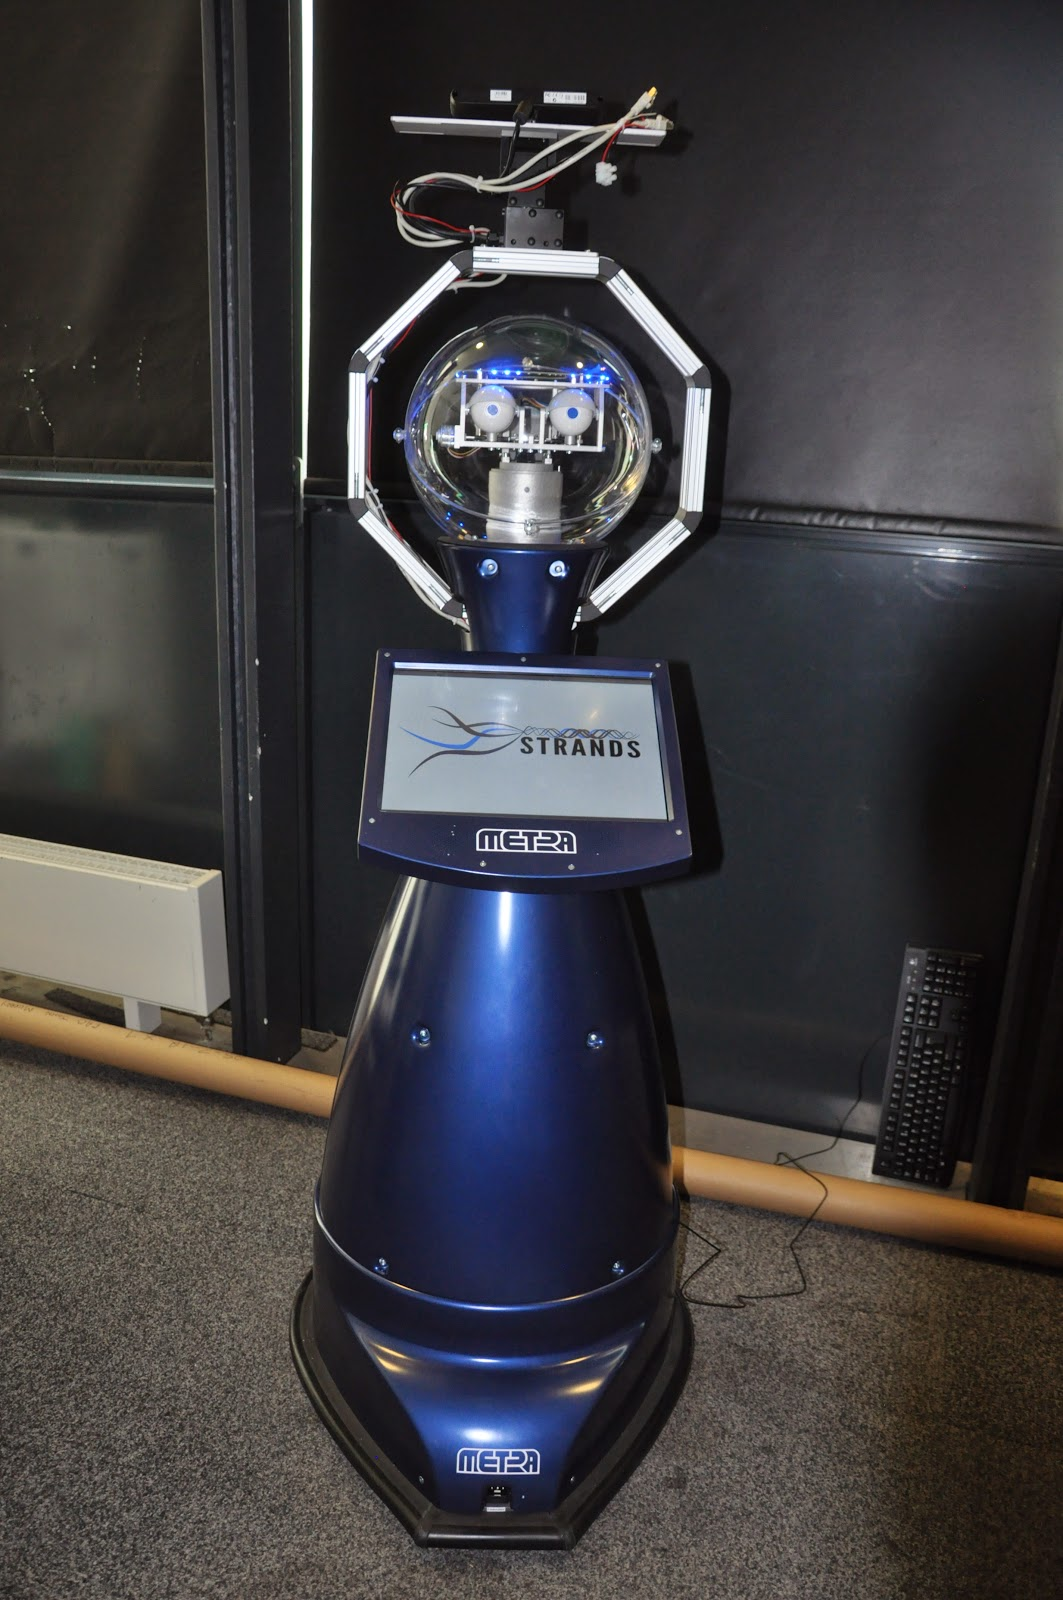
\includegraphics[width=\textwidth]{images/scitos.jpg}
        \caption{}
        \label{fig:scitos-1}
    \end{subfigure}
    ~ %add desired spacing between images, e. g. ~, \quad, \qquad, \hfill etc. 
      %(or a blank line to force the subfigure onto a new line)
    \begin{subfigure}[b]{0.6\textwidth}
        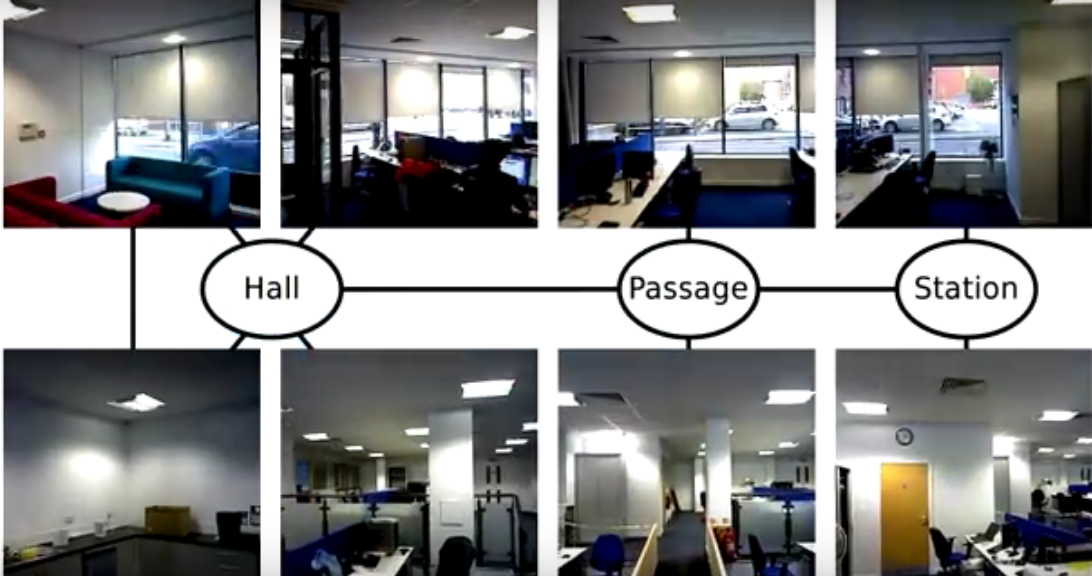
\includegraphics[width=\textwidth]{images/kth-dataset-2.png}
        \caption{}
        \label{fig:robot-view-1}
    \end{subfigure}
    \caption[Brayford dataset collection]{Brayford Dataset collection: SCITOS-G5\footnotemark Robot used for data collection \ref{fig:scitos-1} \protect. Images \footnotemark as seen by the robot at the different rooms in the lab \ref{fig:robot-view-1}}\label{fig:brayford-dataset}
\end{figure}

\footnotetext{\url{ http://www.hanheide.net/2013/06/brand-new-robot.html}}
\footnotetext{\url{https://www.youtube.com/watch?v=aTr9KD4XMGc }}


\section{Experiments}
We conducted our experiments on real data collected by a robot in an office environment. The robot for each room in the office makes observation of its occupancy. The goal of the experiment was to verify that
\begin{itemize}
    \item the robot is able to learn the room occupancy probability.
	\item the resulting model allows for accurate prediction or future occupancy of the room
\end{itemize}

\subsection{Evaluation of Model accuracy}

We evaluated the model accuracy using cross-validation methods on the Brayford dataset. Brayford dataset is extracted from the Witham Wharf RGB-D dataset, both collected as part of the Spatio-Temporal Representations and Activities for Cognitive Control in Long-Term Scenarios (STRANDS) project. 
Witham Wharf RGB-D dataset is used for testing RGB-D localization in changing environments. The dataset consist of RGB-D images collected over eight locations in an open-plan office. The Brayford dataset was extracted from the above dataset by manually annotating the presence of human in the room at the moment. Figure~\ref{fig:brayford-dataset} shows the data collection method. Data was collected using the SCITOS-G5 robot. 



\begin{figure}[htp]
\centering
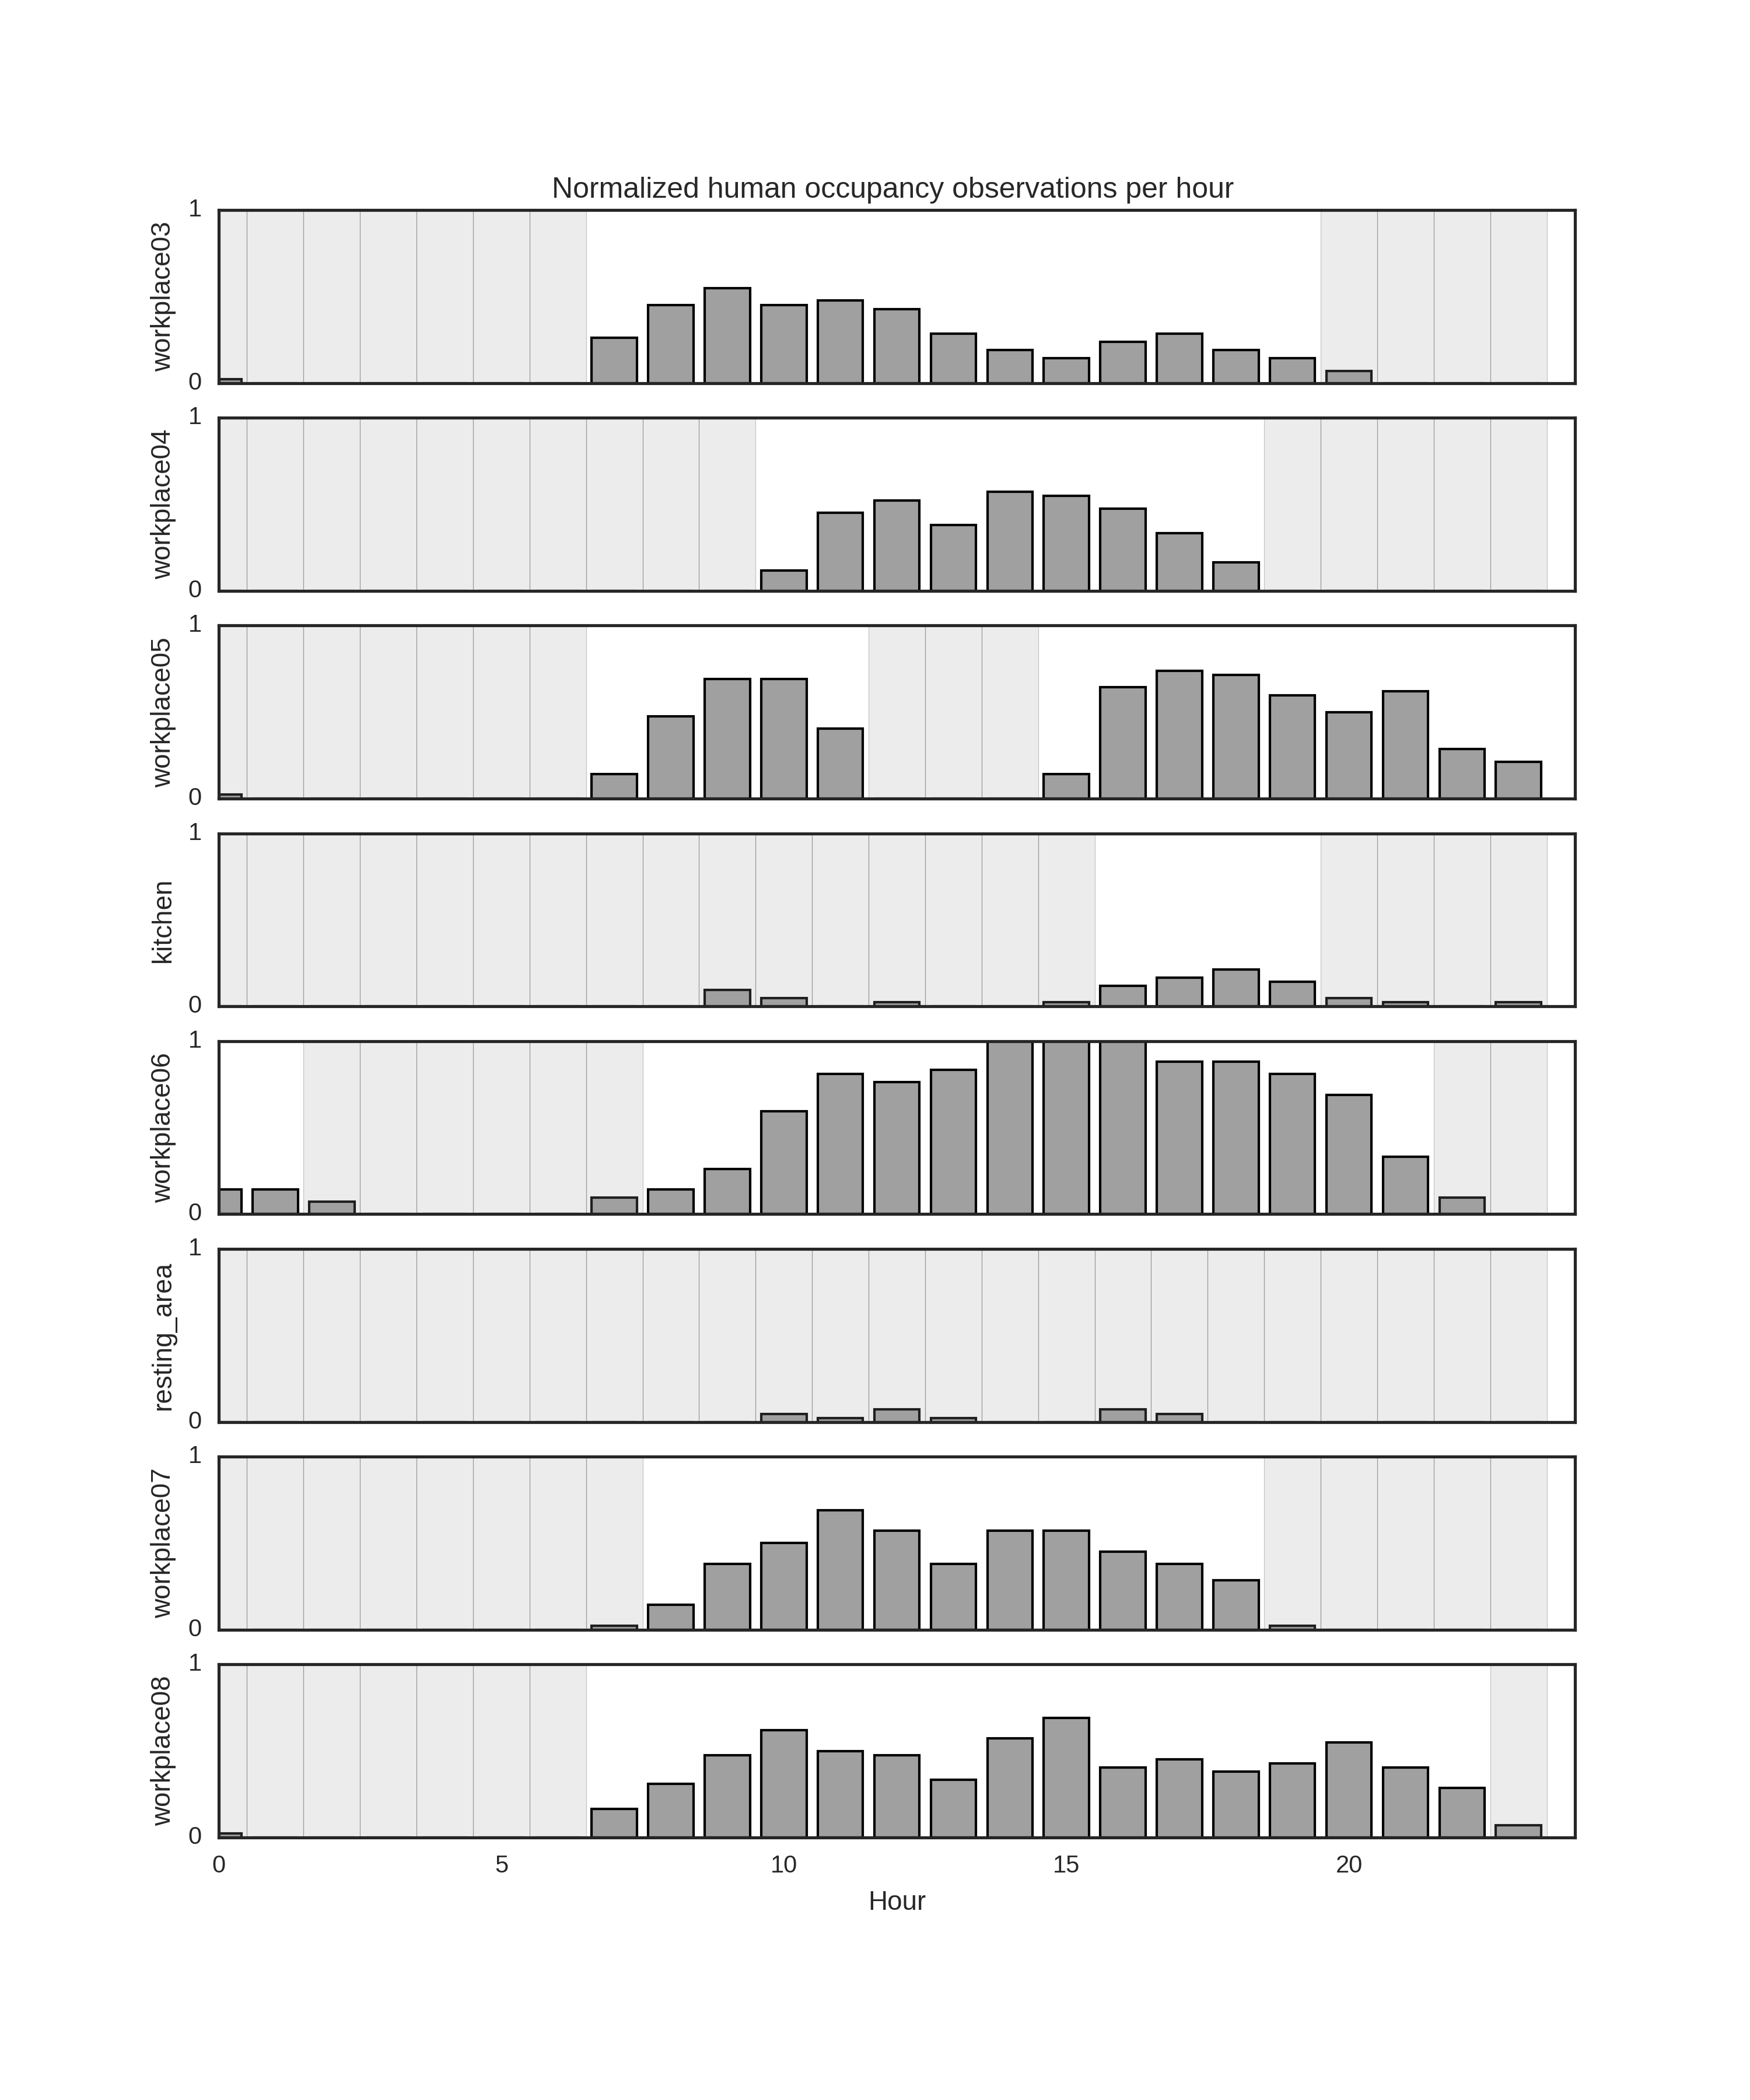
\includegraphics[width=\textwidth]{images/occupancy_hist_withresults.png}
\caption[Brayford Dataset ]{Brayford Dataset: normalized human occupancy per hour per room. The shaded regions are the learned cleaning time period for each room.}
\label{fig:brayford_visualization}
\end{figure}

\FloatBarrier



The dataset is divided in 2 parts the training set and testing set. The training set consist of 7 days of observations, where the robot visits predefined eight locations of the office at a regular interval of 10 minutes each. The testing set consist of another week of observation. Figure~\ref{fig:brayford_visualization} is the bar plot of the observations made by the robot. 



The training dataset was used to learn the parameters of the model while the testing dataset was used to predict and validate the learned models. 
The accuracy results of the 8 rooms is plotted in Figure~\ref{fig:brayford_evaluation} . The model predicts with above \textbf{80\%} accuracy for 3 rooms kitchen, resting area and workplace04 . While accuracy of predictions for other rooms are in the range of 60\% to 80\% .

\begin{figure}[htp]
\centering
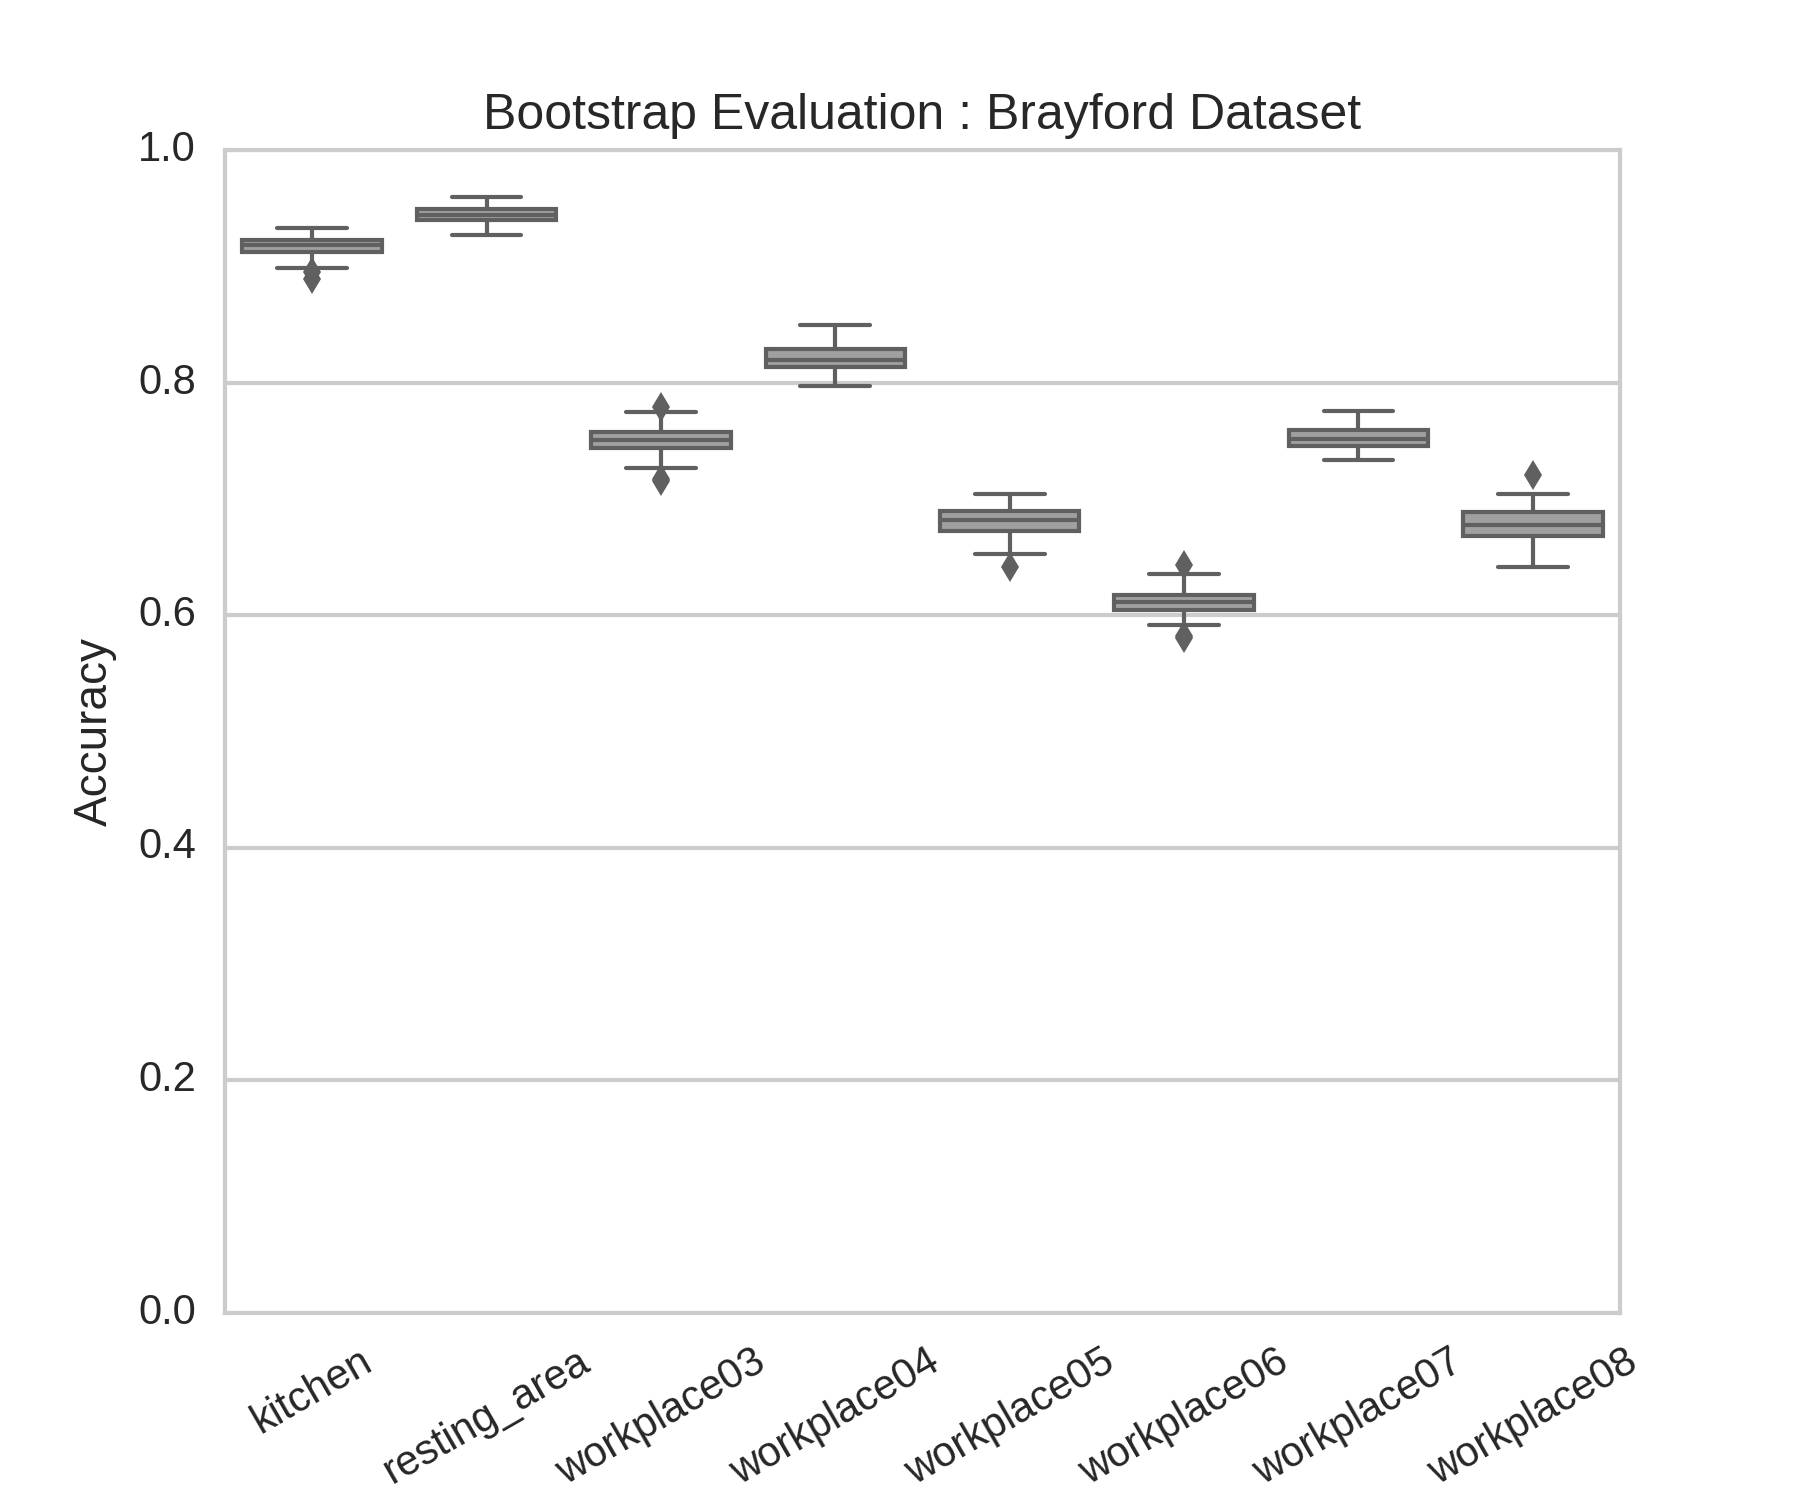
\includegraphics[width=0.7\textwidth]{images/Brayford_dataset_results_evaluation.png}
\caption[Brayford Dataset Evaluation]{Brayford dataset evaluation: Accuracy of the model for different rooms in the office}
\label{fig:brayford_evaluation}
\end{figure}



Based on the learned occupancy parameter for each room, the robot can now determine which are the period of low occupancy and select these time periods for doing its cleaning task. The shaded region in the Figure~\ref{fig:brayford_visualization} are the learned time periods in which the robot can perform cleaning task.
\FloatBarrier

\section{Discussions}

In this chapter, we presented a probabilistic framework for learning the occupancy periods of each rooms. The robot continuously records in its robot memory when and where it saw the users. Now based on the data collected the robot now does an analysis gain knowledge about the occupancy of each room. 

We have used the identical model as discussed in chapter ~\ref{chapter: object} for learning the occupancy parameter. This demonstrates the flexibility of the probabilistic programming in which we can reuse the models to new problems.
From the experiments conducted on real world datasets collected by mobile robots in an open office we can conclude that the model is able to learn accurately the latent occupancy time periods. 
\chapter{Modelling User Location Preferences }
\label{chapter:Human location}
Domestic service robots in future should be able to gather knowledge about all the locations in the home, the user likes to hang around. Additionally they should also know the time period when the users occupy their favourite places. This acquired knowledge of the users location preference shall enable the robots to make informed decisions while assisting the user. For example what time to clean a particular room based on least unoccupied time period or when to turn on the heater of the room. 

In this chapter we focus on this knowledge accession of users location preference based on spatio-temporal observations made by the robot. The advancement in long term autonomous navigation \cite{krajnik_life-long_2015} and the rapid adoption of databases in the robots \cite{niemueller2012generic}, has made the information collection for such knowledge generation possible in service robots. However even with these advancements there are some challenges which still needs to be addressed.  In more details, these challenges are the  (i) modelling users location preference  (ii) prediction of users future locations  (iii) learning all these with sporadic observations made by the robots. 

Significant progress has been made the problem by researchers in the field of human location behaviour, which is to learn the patterns in human location outdoors. Approaches for learning routine mobility  range from purely temporal  (\cite{mcinerney2013modelling, scellato2011nextplace}), spatial  (\cite{gao2012exploring,song2006evaluating}), to a combination  of  both   (\cite{eagle2009eigenbehaviors}). Non-parametric Bayesian methods are also gaining popularity given their ability to refine models as more data arrives. Chen et al.  (2012) used a Gaussian process to model congestion on road networks, while Gao et al.  (2012) used a hierarchical Pitman Yor process to model check-in behaviour on location-based social networks. Indoor human location behaviour was studied by \cite{krajnik_wheres_2015} using Fourier transform methods and Gaussian mixture models. 

While \cite{krajnik_wheres_2015}  work is first step towards learning human mobility behaviour in indoor environments, it failed to address the challenge of sparse dataset in domestic robots. As we have discussed earlier the observations on which the knowledge has to be learned, are sparse. We aim to demonstrate in this chapter that, by using Bayesian models, we can capture the human behaviour patterns in a sparse dataset.

We build Bayesian models which incorporate explicit domain knowledge and the structural knowledge about our data. Human behaviours are periodic in nature with a daily cycle. The models developed use this domain knowledge to extract the patterns emerging from the data caused by periodicity.


\section{Dirichlet Categorical Model }

Dirichlet Categorical (DC) model  is a two-level Bayesian model. The basic idea is that observations of each time period is characterized by a distribution over the possible locations.

In chapter \ref{chapter: object} and \ref{chapter:occupancy} we learned the pattern in the user preference in a single location. For modelling single location based on the presence and absence data we used the Bernoulli distribution to quantify the preference. Here we would like to model the user preference over multiple location in a single model. For modelling more than 2 discrete outcomes, we can use Multinomial or Categorical distribution. In our model we have selected Categorical distribution as the input data to our problem comes sequentially. 

The data are the observed human location $x_{ij}$ for $i = 1 \dots T$ time periods and then $j = 1, \dots , N$  are the observations.  We assume that the latent pattern in the persons location per period are distributed as a categorical distribution. The number of periods $T$ for our model is fixed to 24 corresponding to the number of hours in a day. 

The Dirichlet-Categorical model is the generalization of the Beta-Binomial model to multiple classes of a categorical or multinomial distribution. The conjugate prior for the categorical distribution is the Dirichlet distribution. The model estimates the posterior distribution of $\theta_i$ given our current data and prior beliefs. Our prior beliefs are encoded in the model through the hyper-parameter $\alpha$, which represents pseudo-counts of what we believe the data should look like – typically set as 1's for weak uniform beliefs. The probabilistic graphical model of  DCM is shown in Figure~\ref{dcm}

\noindent
\begin{figure}[htp]

\begin{minipage}{0.3\textwidth}
\centering

\tikz {
\node [const]                   (alpha) {$\alpha$};
\node [below=of alpha, latent]   (theta) {$\theta_i$};
\node [below=of theta, obs]      (x)     {$x_{ij}$};
\edge {alpha} {theta};
\edge {theta} {x};
\plate {trials} { (x)} {j location};
\plate {bags} { (theta) (x) (trials)} {i time};
}

\end{minipage}%
\begin{minipage}{0.7\textwidth}

\begin{equation*}
	\alpha = <1, 1, .... , 1 > 
\end{equation*}
\begin{equation*}
	\theta_i  \sim Dirichlet (\alpha)
\end{equation*}
\begin{equation*}
	x_{ij} \sim Categorical (\theta_i)
\end{equation*}
\end{minipage}
\caption[Dirichlet categorical graphical model representation]{Graphical model representation of DCM. The boxes are ``plates" representing replicates. The outer plates represents hours of a day, while the inner plate represents the choice of locations within each hour.}
\label{dcm}
\end{figure}

With the graphical model, the dependencies among the many variables can be captured concisely. The boxes are ``plates” representing replicates. The outer plate represents the hours of the day, while the inner plate represents the repeated choice of locations within each hour. Thus:

	$\alpha$ is  parameter of the dirichlet prior on per-period location distribution, 
	
	$\theta_i$ is the location distribution for period $i$  ,
	
	$x_{ij}$ is the observed location of the person in period $i$.
	
The $ x_{ij}$ are the only observable variables, and the other variables are latent variables. 

\section{Hierarchical Dirichlet Categorical Model}
\label{sec: HDCM}

Observations made only by a domestic robot using internal sensors and not using any external sensors creates the serious problem of sparsity. There are very much likely that some time periods there will be no observations available to learn. Maximum likelihood estimates of the categorical parameters assign uniform probability to the locations in these time periods. The standard approach to cope with this problem is to sharing statistical strength between time periods: it is as if the location we observe for each time period also provides weaker indirect location relevant to other time periods. In machine learning and statistical science this phenomenon is often called \emph{learning to learn} or \emph{transfer learning}. Intuitively, knowing something about the location of person in the 9'o clock can help in gaining some information at 10'o clock. 

By placing a Dirichlet hyper-prior on the several Dirichlet parameter we obtain the  Hierarchical Dirichlet Categorical  (HDC) model. The hyper-prior makes it possible for sharing the learned knowledge from one prior to another. Thus learning about the location pattern at a higher level of abstraction helps to share it with the lower levels which have no observations.

The probabilistic graphical model of  hierarchical model is shown in Figure \cite{hdcm}

\noindent
\begin{figure}[htp]

\begin{minipage}{0.3\textwidth}
\centering

\tikz {
\node [const]                    (alpha) {$\alpha$};
\node [below=of alpha, latent]   (beta)  {$\beta$};
\node [below=of beta, latent]    (theta) {$\theta_i$};
\node [below=of theta, obs]      (x)     {$x_{ij}$};
\edge {alpha} {beta};
\edge {beta} {theta};
\edge {theta} {x};
\plate {trials} { (x)} {j location};
\plate {bags} { (theta) (x) (trials)} {i time};
}

\end{minipage}%
\begin{minipage}{0.7\textwidth}

\begin{equation*}
	\alpha = <1, 1, .... , 1 > 
\end{equation*}
\begin{equation*}
	\beta \sim Dirichlet (\alpha)
\end{equation*}
\begin{equation*}
	\theta_i  \sim Dirichlet (\beta)
\end{equation*}
\begin{equation*}
	x_{ij} \sim Categorical (\theta_i)
\end{equation*}
\end{minipage}
\caption[Hierarchical dirichlet categorical graphical model representation]{Hierarchical Dirichlet Categorical Model. The boxes are ``plates" representing replicates. The outer plates represents hours of a day, while the inner plate represents the choice of locations within each hour.}
\label{hdcm}
\end{figure}

The model can be explained as:

	\boldmath{$\alpha$} is  constant dirichlet prior for the hyperprior, 
	
	$\beta$ is a Dirichlet hyperprior,
	
	$\theta_i$ is the location distribution for period $i$  ,
	
	$x_{ij}$ is the observed location of the person in period $i$.
	
Thus we have categorical variables dependent on multiple priors sharing a hyperprior.


\section{Experiments}

We give an empirical performance analysis of the above models to determine their capabilities of learning user behaviour and preferences. We first conducted experiments on synthetic dataset to verify if the evaluate the proposed models can learn and the number of observations required for making accurate predictions. Then we compare the DC and HDC models on their capabilities to learn when there is absence of data. Finally we evaluate the models predicting capabilities on a real dataset collected about human location in a home.

The goal of the experiments are to verify 
\begin{itemize}
	\item the robot is able to learn users location preferences.
	\item performance of HDC model compared to DC model.
	\item performance of HDC model with standard machine learning algorithms
	\item search time to locate a person.
\end{itemize}


\section{Model Learning Validation}

Before we start learning on the real dataset we want to validate the proposed models using synthetic dataset. The synthetic dataset consist of observations made by a robot generated using known ground truth probabilities. The models learn using the synthetic dataset and generate the learned probabilities. The distance between the learned probability and ground truth probability is used to quantify the learning of the model. 

\subsection{Simulated Dataset: Kitchen Object Dataset}

To demonstrate the learning in the proposed approach we have generated a kitchen object dataset. The dataset consist of simulated observations of a cup in a kitchen environment made by a domestic robot \cite{fig:eval_cup}. The robot can scan 4 locations in the kitchen: sink, counter-top, stove and cabinet. The time of the scan is discretized into 3 times of the day: morning, afternoon and night. 

The generative process for each possible observation in the dataset 
\begin{itemize}
    \item Choose $ \theta \sim Dirichlet (\alpha)$  (Distribution of object over location-time)
    \item Choose randomly the time period $i$.
	\item Choose the location $x_n$ $\sim$ Categorical$ (\theta_i)$ , where the object was observed.
	\end{itemize}

Ground truth of the distribution in the object location distribution over time in shown in Figure \ref{absent-gt}. The figure represents the hinton plot of the underlying Dirichlet distributions. Hinton plot are a way of visualizing probabilities. The size of the white square in the plot quantifies the belief of the probability. Higher the size of the box higher the probability. Thus for probability 1 we have a complete white box and gray means 0 probability. In the ground truth probability in Figure \ref{fig:eval_gt} the each row represents the distribution of the object cup at the particular time period. We see a big white box at location:sink and time:night on the bottom left of the plot, while all other boxes for row night are comparatively small. This signifies that the box is more likely to be found in the cabinet in the night than the other places.  We evaluate our models on these synthetic observations.

\begin{figure}
    \centering
    \begin{subfigure}[b]{0.4\textwidth}
        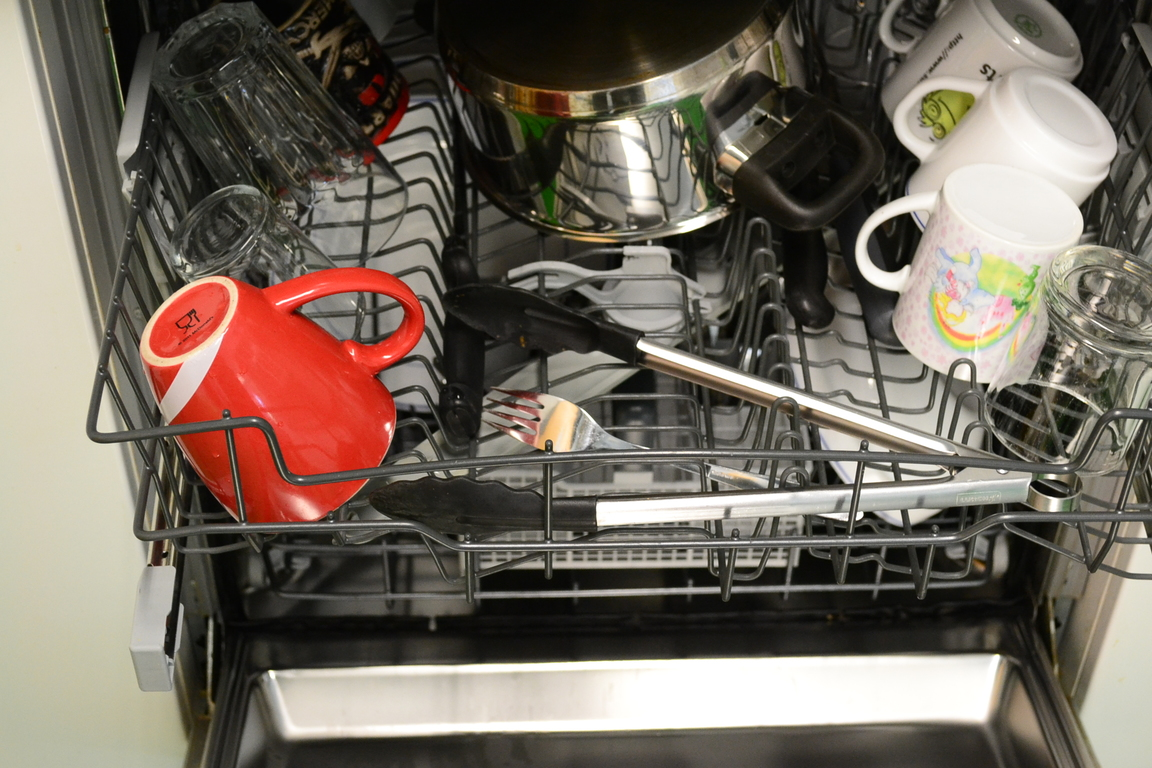
\includegraphics[width=\textwidth]{images/cup_dishwasher.jpg}
        \caption{}
        \label{fig:eval_cup}
    \end{subfigure}
    ~ %add desired spacing between images, e. g. ~, \quad, \qquad, \hfill etc. 
      % (or a blank line to force the subfigure onto a new line)
    \begin{subfigure}[b]{0.5\textwidth}
        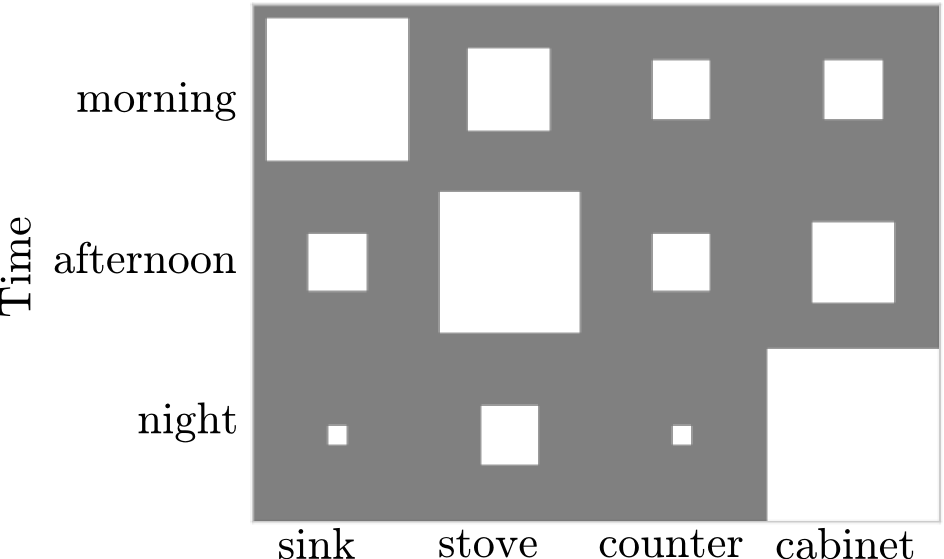
\includegraphics[width=\textwidth]{images/eval_ground_truth.png}
        \caption{}
        \label{fig:eval_gt}
    \end{subfigure}
    \caption[Model Validation dataset generation]{Simulated dataset generation of the cup in different location at different times of the day. Simulated cup locations ground truth probability distribution.
The x-axis represents the locations the y axis represents the timezones. The size of the white box indicates the probability of the object presence.}
\label{}
\end{figure}




\subsection{Posterior Probability Check}
The first method was to visually compare the learned probabilities with the ground truth.  Figure~\ref{fig:eval_gt} we can visually analyse the difference between the learned models of both DC model and HDC model. The leftmost plot \ref{fig:eval_gt} as explained above is the ground truth probabilities from which the observations were generated. We generated a dataset with \textbf{100} observations. The models use the observations and creates its posterior distribution. The middle plot \ref{fig:eval-dc} is the learned posterior probabilities using the DC model while the last plot \ref{fig:eval-hdc} is the posterior probabilities using the DC model presented in this chapter. 

Visually we can observe from the plots both the posterior probabilities of both the models are similar to the ground truth probabilities. Thus we can conclude that the proposed models are converging to the true probabilities. In the next section we quantitatively compare the models using different data size.

\begin{figure}
    \centering
    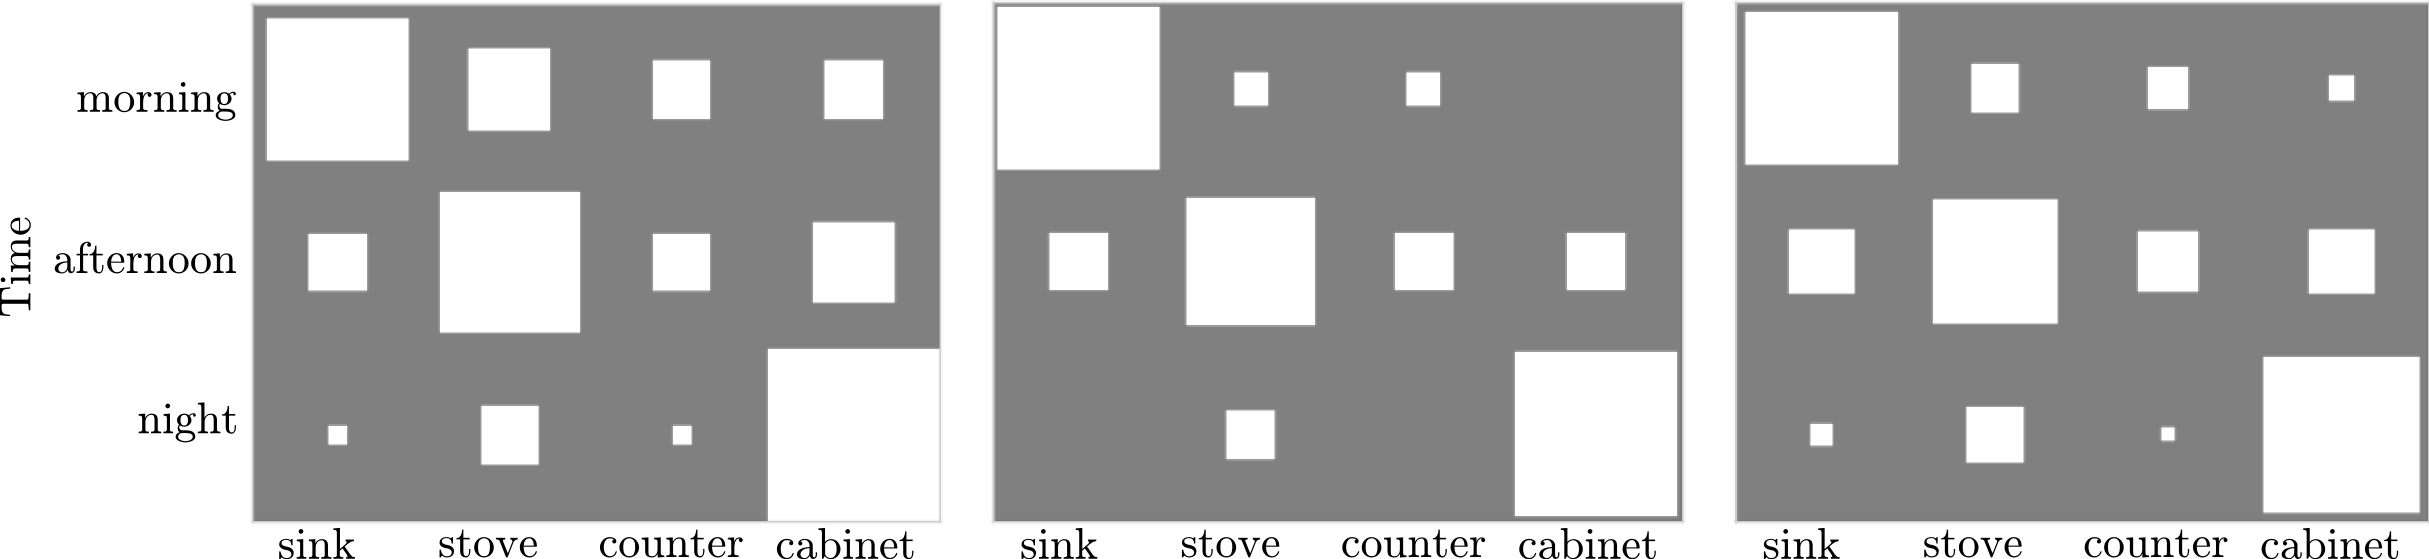
\includegraphics[width=\textwidth]{images/eval_gt_DC_HDC.png}
       
    \begin{minipage}[t]{.35\textwidth}
    %\centering
    \subcaption{Ground Truth}\label{fig:eval_gt_2}
    \end{minipage}%
    \begin{minipage}[t]{.3\textwidth}
    %\centering
    \subcaption{DC model}\label{fig:eval-dc}
    \end{minipage}
    \begin{minipage}[t]{.25\textwidth}
    %\centering
    \subcaption{HDC model}\label{fig:eval-hdc}
    \end{minipage}

\caption[Posterior probabilities of DC and HDC ]{Posterior probabilities of the models : \ref{fig:eval_gt_2} is ground truth of the distribution. \ref{fig:eval-dc} is the learned distribution using the DC model. \ref{fig:eval-hdc} is the learned distribution using the HDC  model . The x-axis represents the locations the y axis represents the timezones. The size of the white box indicates the probability of the object presence }\label{fig:eval-dc-hdc}
    
\end{figure}

\section{Model Comparison}

The goal of the experiments is to empirically validate both Dirichlet-Categorical and Hierarchical-Dirichlet-Categorical model 
learning using different data size. We also validate that HDC can compensate  for lack of observations in some time period by sharing information.

We employ two methods for evaluating the performance of the developed models on the synthetic dataset. We use the adopted Bhattacharyya distance \cite{bhattacharyya1946measure} and Kullback–Leibler divergence \cite{kullback1951information}  (KL Divergence)to quantify the distance between the simulated and the learned Dirichlet distribution.   

\subsection{Bhattacharyya Distance}
Bhattacharyya distance measures the similarity of two discrete or continuous probability distributions. The distance ranges from 0 to $\inf$ with \textbf{0} meaning both probabilities are identical. The  adopted Bhattacharyya distance \cite{rauber2008bhattacharyya} for comparing dirichlet distributions is given by :
\begin{multline}
	D_B (Dir_a (x_1, \dots ,x+n), Dir (y_1, \dots , y_n)) = \nonumber\\
	 \Gamma \Bigg ( \frac{1}{2}  \sum_{i \in {1, \dots, n}} x_i +  \frac{1}{2}\sum_{i \in {1, \dots, n}} y_i\Bigg) + 
	\frac{1}{2}  \sum_{i \in {1, \dots, n}} \Gamma  (x_i) + 
	\frac{1}{2}  \sum_{i \in {1, \dots, n}} \Gamma  (y_i) - \\ 
	\sum_{i \in {1, \dots, n}} \Gamma \bigg (\frac{1}{2}  (x_i + y_i) \bigg) - \frac{1}{2}  \Gamma \Bigg (  \sum_{i \in {1, \dots, n}} x_i \Bigg) + \frac{1}{2}  \Gamma \Bigg ( \sum_{i \in {1, \dots, n}} y_i\Bigg)
\end{multline}

\subsection{Kullback–Leibler Divergence}
Similarly KL divergence also measures the similarity of two discrete or continuous probability distributions. Even for KL divergence, 0 signifies both probabilities are identical.  
The KL divergence between two distributions $p$ and $q$ is given by
\begin{equation*}
	KL (p||q) = \int p (x) \log \frac{p (x)}{q (x)} dx = \left < \log \frac{p (x)}{q (x)}  \right>_{p (x)}
\end{equation*}

Lets suppose we have two Dirichlet distributions $p$ and $q$ with parameters $\alpha$ and $\beta$ respectively, then the KL divergence between Dirichlet distributions\cite{kurt2013} is given by
\begin{equation*}
	\begin{split} 
 KL (p||q) &= \log \Gamma (\alpha_0) - \sum_{k=1}^K \log \Gamma (\alpha_k)   
 - \log \Gamma (\beta_0) \\ &+ \sum_{k=1}^K \log \Gamma (\beta_k)  + \sum_{k=1}^K  (\alpha_k – \beta_k)  (\psi (\alpha_k)-\psi (\alpha_0)) 
\end{split}
\end{equation*}


The only difference being that KL divergence is unsymmetrical while Bhattacharyya distance is symmetric. 

\subsection{Results}
We generated dataset with increasing number of observations from 20 to 800. For each observation set we trained both the models and their corresponding distance with the ground truth were recorded. The process was repeated 100 times for each sample set.

\begin{figure}[htp]
\centering

\begin{subfigure}{.45\textwidth}
  \centering
  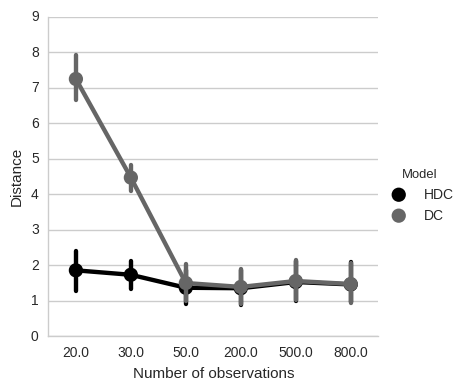
\includegraphics[width=\linewidth]{images/Eval-HDC-Bhattacharya-Distance.png}
    \caption{Bhattacharyya distance}
\end{subfigure}
\begin{subfigure}{.45\textwidth}
  \centering
  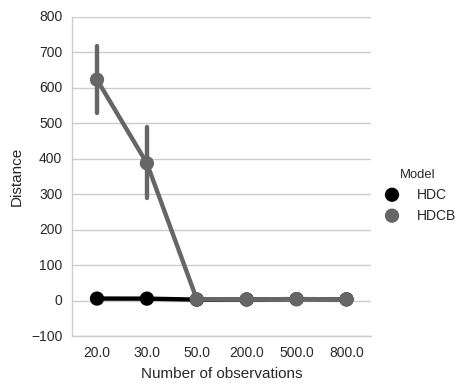
\includegraphics[width=\linewidth]{images/Eval-DC-KL-Distance.png}
    \caption{Kullback–Leibler divergence}
\end{subfigure}

\caption[DC, HDC Model Validation]{Measure of the distance between the learned probabilities and ground truth for models DC and HDB. The x-axis represents the different sample size.}
\label{fig:eval-B-KL-evaluation}
\end{figure}

Distances between the learned and the ground truth probabilities, learned using increasing number of observations is depicted in Figure~\ref{fig:eval-B-KL-evaluation}. The left plot is the Bhattacharyya distance while the right plot is the KL distance. We can observe that with increasing number of observations the distance is reduced. With around 50 observations both the models  completely converged with the ground truth.  

From the figure we can also conclude that when the observations are very few the HDC model performs better than the DC model. This validates that when some time periods which dont have enough observations the hyper prior added in hierarchical model shares information between time periods. HDC model performs better than DC model when the observations are few but as the observations increase there is no considerable difference in their learnings.

\section{Model Accuracy}

We have validated the working of the models on synthetic dataset in this section we validate HDC model on real world dataset. The aim of the experiments is to learn human location preference on real world dataset of location of a human in a house. We employ two methods for evaluating the performance of preference learning models. In addition to the traditional \emph{accuracy} measurements, we also evaluate the models based on the \emph{mean time to find the person}.  In the following section we explain the data collection procedure, data processing to information and then the two evaluation procedures.
 
\subsection{Aruba Dataset}
In our thesis, we have used a  publicly-available  dataset Aruba, published by the Lincoln Center for Autonomous Systems (LCAS). The dataset is of a person's location in a home collected at a smart apartment by the Center for Advanced Studies in Adaptive Systems (CASAS) \cite{aruba} .

The testbed where the dataset was collected is a  three-bedroom apartment located on the Washington State University that is part of CASAS smart home project \cite{aruba}. 


\begin{figure}
    \centering
    \begin{subfigure}[b]{0.4\textwidth}

        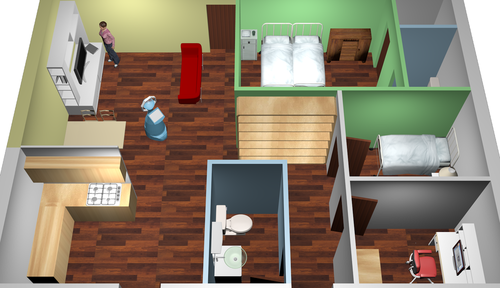
\includegraphics[width=\textwidth]{images/aruba-flat.png}
        \caption{Aruba apartment visualization}
        \label{aruba}
    \end{subfigure}
    ~ %add desired spacing between images, e. g. ~, \quad, \qquad, \hfill etc. 
      % (or a blank line to force the subfigure onto a new line)
    \begin{subfigure}[b]{0.5\textwidth}
        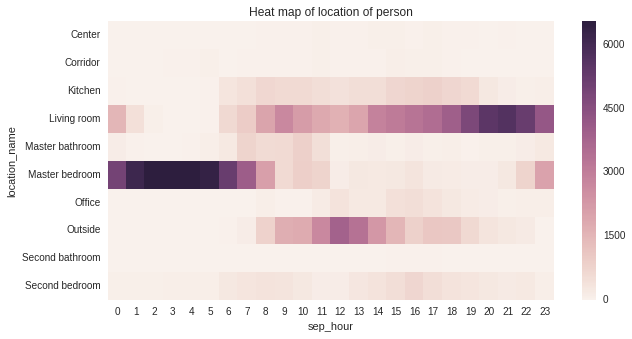
\includegraphics[width=\textwidth]{images/aruba-data.png}
        \caption{Heatmap}
        \label{fig:eval_gt}
    \end{subfigure}

    \caption[Aruba apartment visualization]{Aruba apartment visualization and Aruba dataset heatmap. In the heatmap, the x-axis are the locations of the home, y-axis are the hours of the day. The intensity of the color in each box indicates the number of times the person is present in that location. Higher the intensity means more time is spent by the person in that location at that time.}
    \label{aruba-visual}
\end{figure}

As shown in Figure~\ref{aruba}, the smart apartment test bed includes three bedrooms, one bathroom, a kitchen, and a living / dining room.  The apartment is equipped with motion sensors distributed approximately 1 meter apart throughout the space. The Aruba dataset was extracted from these motion sensor dataset provided by CASAS. The dataset contains the location of a person in the apartment every minute for 16 weeks.

We process the dataset and  order it as a  (hour,location) tuple. We visualize the dataset as a heatmap over locations distributed over different periods. As explained in chapter~\ref{sec:Problem formulation}, we try to learn daily patterns by dividing the observations into per hour periods. As we can see there are some prominent patterns present which can be learned. For example the usage of the bedroom, living room, outside and kitchen.

A histogram visualization of the observations over different location in the home is show in Figure~\ref{aruba-hist}

\begin{figure}[htp]
\centering
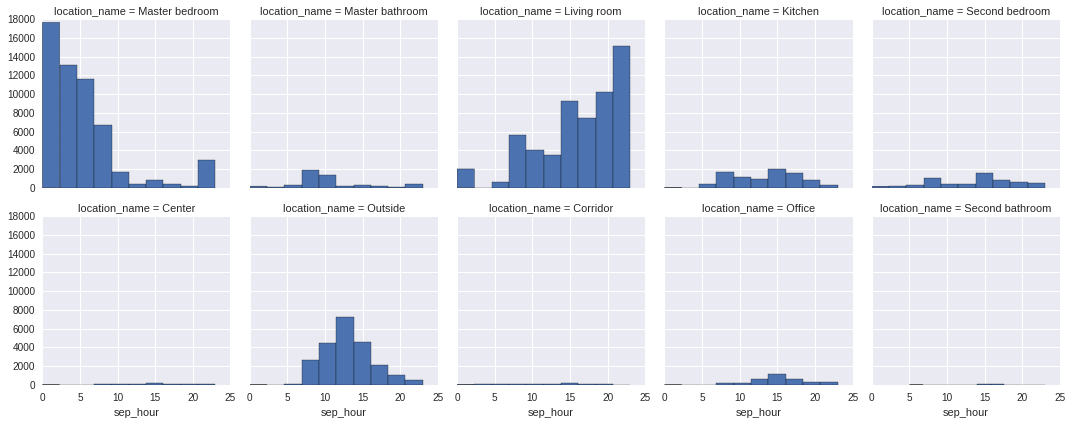
\includegraphics[width=\textwidth]{images/aruba-hist.png}
\caption[Aruba dataset histogram]{Aruba Dataset Histogram : Each box corresponds to histogram of each locations. The x - axis represents the time of the day (0-24) }
\label{aruba-hist}
\end{figure}


\subsection*{Sparsification}
Aruba dataset is a large dataset as compared to an person location dataset we assume the robot will be able to generate. The Aruba dataset has recordings of every minute for 118 days, which is 161280 readings.
On the contrary the assumed dataset which will be collected by the robot by autonomously roaming in a home will be just 3-5 readings per day.
So for simulating the sparsity in the object location dataset we will sparsify the ARUBA dataset by random selecting only selecting 3-5 readings each day.

After sparsification by randomly selecting 5 readings per day the dataset is reduced to 590 observations. The heatmap the of the sparsified dataset is shown in Figure~\ref{aruba-reduced-hist}. 

\begin{figure}[htp]
\centering
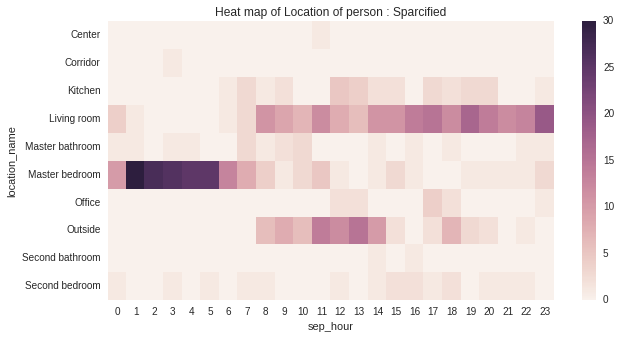
\includegraphics[width=\textwidth]{images/aruba-reduced-heatmap.png}
\caption[Aruba sparcified dataset heatmap]{Aruba sparcified dataset heatmap :The x-axis are the locations of the home, y-axis are the hours of the day. Compared to the complete observations the sparcified data set the patterns are not distinct}
\label{aruba-reduced-hist}
\end{figure}

\FloatBarrier


\subsection{Comparison With State-Of-Art Machine Learning Algorithms}

In this section we evaluate the predictive capabilities of our learned model. The accuracy of the predictions are measured and then compared with other state of the art machine learning algorithms. Two state-of the-art machine learning algorithms: Support Vector Machine (SVM)\cite{boser1992training, cortes1995support} and Random Forest \cite{breiman2001random, geurts2006extremely}. Scikit-learn \cite{sklearn_api} implementation of the algorithm were used for testing.

The goal of learning users location preference is to predict the location of the user based. We interpret the problem as a supervised machine learning with known input and outputs.In supervised learning the data comes a finite learning set $L =  (X, y)$ where, $X = input values$ and $y = output values$. 
For our problem statement the input is single feature, the time of the observation $X = [time]$, the output is the location of the person $y=[location]$

The learning was conducted using training set of different sizes, ranging from 0.0003\% (484 observations i.e. around 5 observations per day by the robot) to 0.2\% (32256 observations) of the dataset. The remaining data was used as testing set. The accuracy score for the classification is plotted in Figure~\ref{fig:SVM_vs_DCM}. 

\begin{figure}
    \centering
    \begin{subfigure}[b]{0.44\textwidth}
        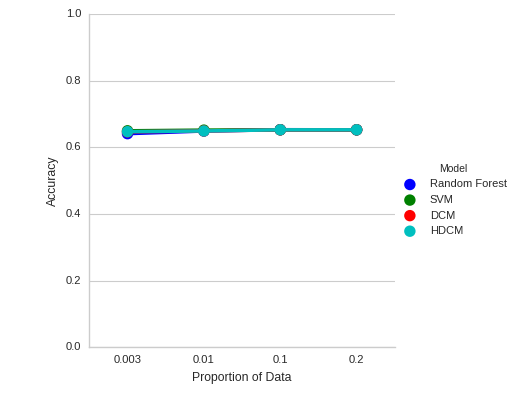
\includegraphics[width=\textwidth]{images/svm_vs_HDCM.png}
    \end{subfigure}
    \begin{subfigure}[b]{0.44\textwidth}
        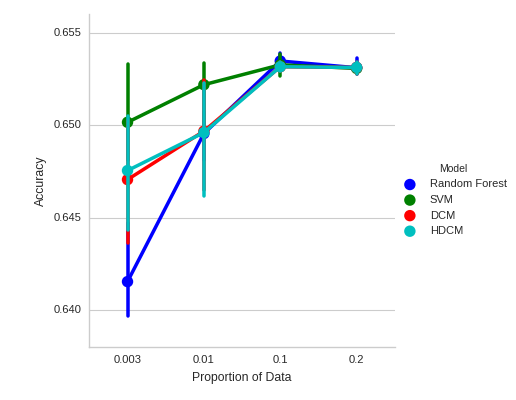
\includegraphics[width=\textwidth]{images/svm_vs_HDCM_zoomed.png}       
    \end{subfigure}
    
    \caption[Comparison with SVM and Random Forest]{ Comparison with SVM and Random Forest. The right plot is the zoomed view between 0.64 to 0.65}
    \label{fig:SVM_vs_DCM}
\end{figure}

As per the accuracy plot there is no considerable difference between the accuracy of  SVM, Random Forest, DC and HDC . Also the maximum accuracy is around 0.64\% , which doesn’t increase even with increasing number of observations. 


\subsection{Search time evaluation}
The models were also evaluated on the basis of the \emph{search time} to find the person. As mentioned above the goal of modelling human presence is to predict the persons location and reduce the time of search. Thus by calculating the time required to search the person based on the predictions of the model we can evaluate the accuracy of the learning.

\cite{krajnik_wheres_2015} in their seminal paper have proposed a path-planning search algorithm. This algorithm is used to determine the shortest path to be taken by the robot based on each locations probability. Thus it goes first to the most probable location first, then to other locations in decreasing order of the probabilities. \cite{krajnik_wheres_2015} solve the problem of learning preference of user location using temporal models. Two temporal models, frequency map enhancement  model  (FreMEn) and periodic Gaussian model (PerGaM) were used to learn the location preferences. 

We compare our developed model HDC along-with the FreMEn model based on the search time. A 'Static' model represented by static probability is used as a reference. Out of the 16 weeks of the Aruba dataset, first 4 weeks were used by \cite{krajnik_wheres_2015} to learn the models and last 12 weeks were used for testing. While in our case we learned using the sparse Aruba dataset  (~550 observations), and testing using same the last 12 weeks as above.

\begin{figure}[htp]
\centering
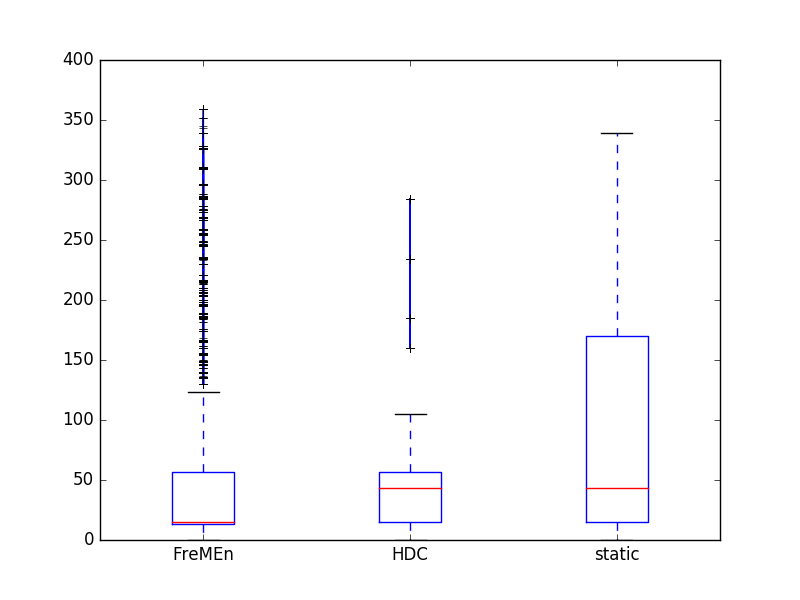
\includegraphics[width=\textwidth]{images/box_plot_fremen_hdc.png}
\caption[Search time evaluation]{Search times for different models}
\label{fig:search_time}
\end{figure}

As shown in Figure~\ref{fig:search_time} that compared to the stationary models the temporal model and our Bayesian models perform better in search time. The average search time of the temporal models are better than the Bayesian model.

\section{Discussions}

In this chapter, we presented probabilistic model to learn user location preferences.  In chapter \ref{chapter:occupancy} the models captured knowledge about each location separately, while in this chapter the models are able to capture knowledge about multiple locations in a single model. 

In an extensive experiments on synthetic dataset, we found that our model is capable of learning underlying patterns in user preferences. In first set of experiments we did a sanity check of our learning by visualizing the learned probability. Then we compared DC and HDC model and validated that addition of a hyper-prior improves learning when the observations are sparse. Furthermore, we evaluated the performance of the models predicting capability on a real world dataset, where the predictive accuracy results were around 63\% . The reason for such low accuracy result even with increasing number of dataset, can be explained by \cite{Bishop20120222} reasoning of ``Large" dataset. The author explains that learning is bad in some computationally large  (size) dataset as their statistical size in relation to the model is small. For example, consider a dataset with single input variable and single output variable with linear relationship. In such a dataset the model can learn with modest (20) examples even in the presence of noise. Such a dataset is computationally small but statistically large. However, a image dataset with millions of images for doing object detection is computationally large but statistically small, as it may contain only a tiny fraction of the different possible combinations. The Aruba dataset can be described as a computationally large but the statistically small dataset.

Finally, we compared the search time required by the robot to find the person in the home. The average search time of the model is reduced than the static search timings, but the median search time is very high as compared to the temporal model, FreMEn \citep{krajnik_wheres_2015}. One of the reasons can be that our models had a hour level dataset while FreMEn was learned at minute level dataset. Thus by learning user preferences the robot can make informed decisions that decrease the search time.
% section   (end)






\chapter{Absence of Information is also Knowledge}

This chapter presents an approach to the problem of learning object placement habits of humans in an occluded environment. Generally in domestic environments like our home, we humans prefer to store our food, cooking equipment, silverware and dishes inside closed cabinets like drawers, cupboards and refrigerators. This causes high level of occlusion for data collection.

We assume there is a domestic service robot which while interacting in human environments records all the information generated using vision sensor.
So for a domestic robot with only camera as a sensor, the chances of observing  these objects inside closed cabinets is drastically reduced.

\begin{figure}[htp]
\centering
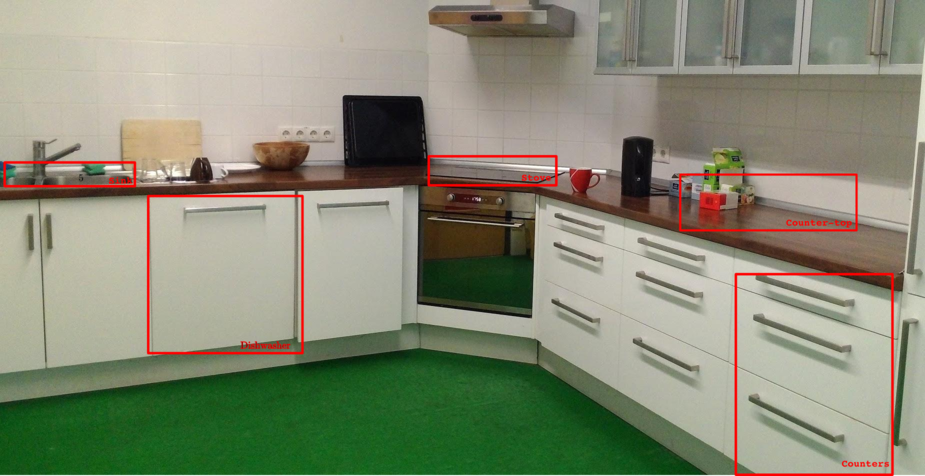
\includegraphics[width=0.8\textwidth]{images/kitchen_crop_ano.png}
\caption{Kitchen environment with occluded spaces}
\label{fig:kitchen occluded}
\end{figure}

The basic requirement of machine learning is data, from which information and knowledge can be learnt. But in highly occluded environments like kitchen its difficult for a domestic robot to make an observation of the object and record the object location.  Hence our hypothesis that we can learn knowledge about object locations quantitatively i.e. learning patterns from the data observed, becomes a herculean task to prove.

An alternative approach to counter the sparsity of data is by recording the absence of the object in visible locations and learning knowledge about where objects are not located. Consider an motivating example, as depicted in Figure \ref{fig:alllocations} . Here, a mobile robot is in a kitchen in the morning. The following locations can be scanned by the robot: kitchen-sink, counter-top and stove, while the cabinets, dishwasher and refrigerator are occluded. The robot will make observations of cup and kettle on counter-top , spoon on the sink top. Assume that the robot is also learning object locations of cooking pot. If the robot only records the observed objects then there is no data recorded for the cooking-pot and no knowledge is learned about the cooking-pot. \emph{A possible solution is to even record the \textbf{absence} of cooking-pot on the visible locations}. From this the robot can learn that the cooking-pot is less probable to be on the kitchen-sink, counter-top and stove during morning time. Supplementary the robot can also learn that there is higher probability for the cooking-pot being in the cabinet or dishwasher.

\begin{figure}
    \centering
    \begin{subfigure}[b]{0.3\textwidth}
        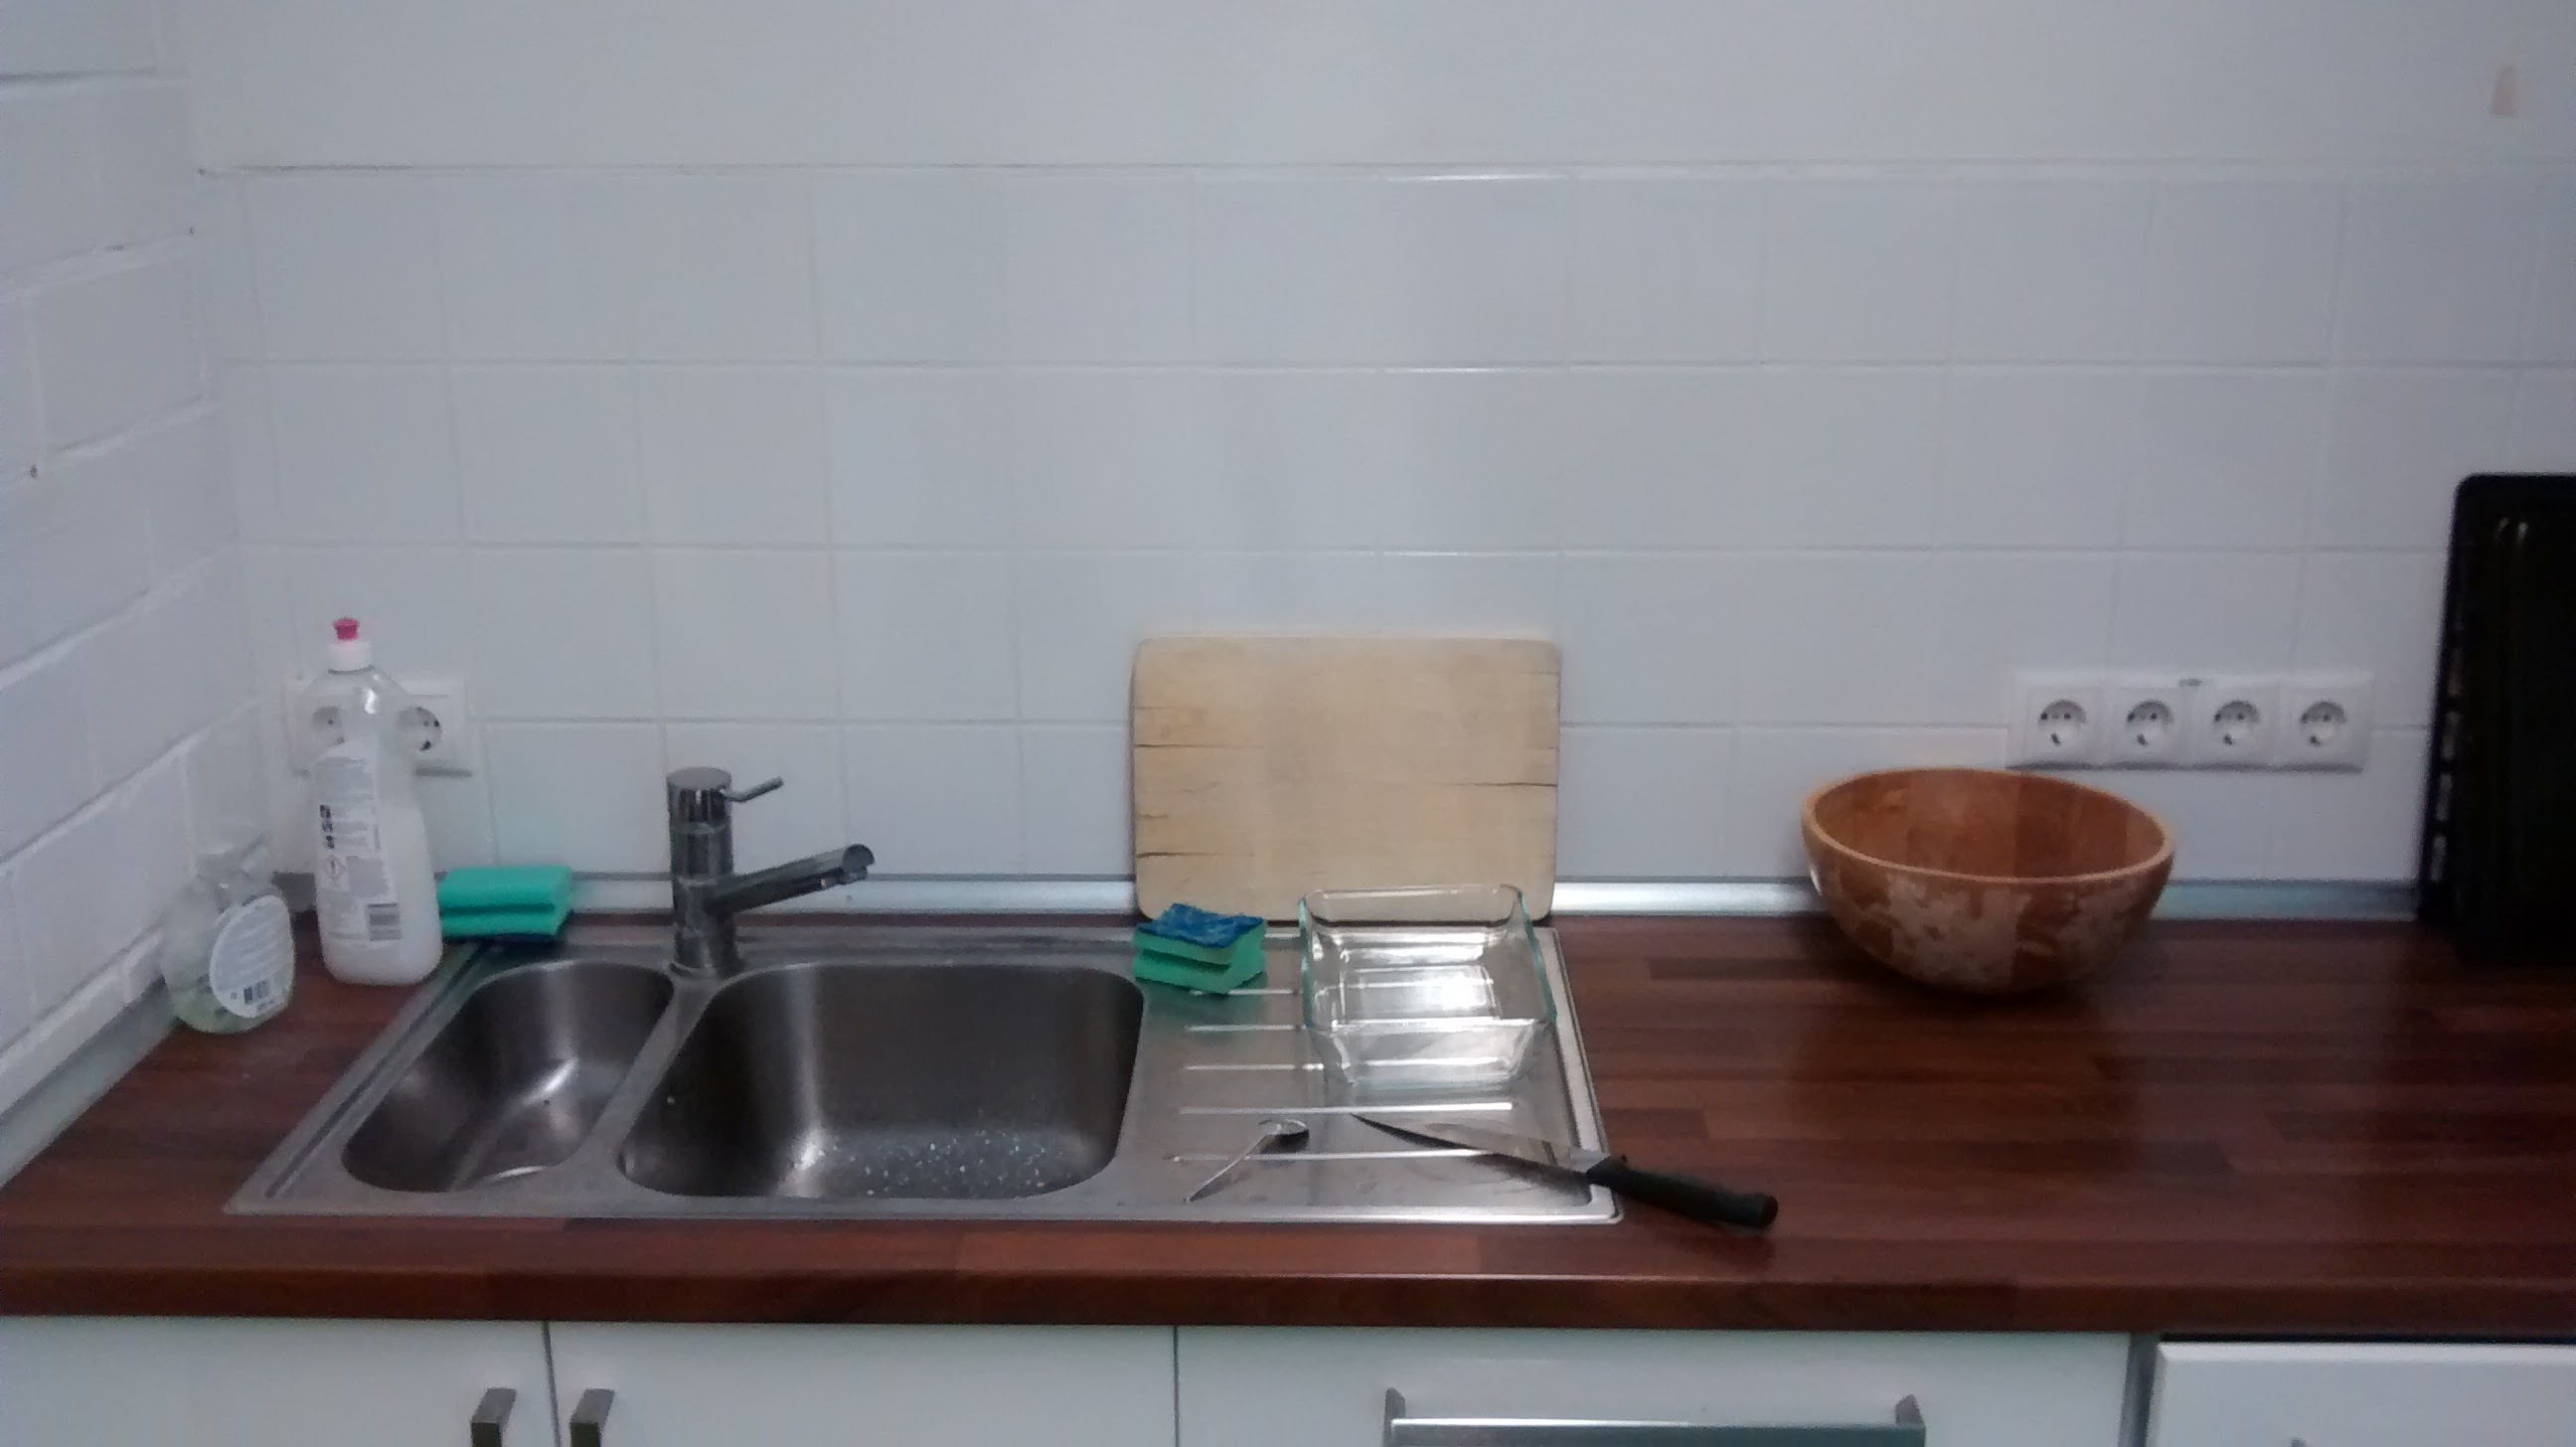
\includegraphics[width=\textwidth]{images/sink.jpg}
        \caption{Sink}
        \label{fig:sink}
    \end{subfigure}
    ~ %add desired spacing between images, e. g. ~, \quad, \qquad, \hfill etc. 
      %(or a blank line to force the subfigure onto a new line)
    \begin{subfigure}[b]{0.3\textwidth}
        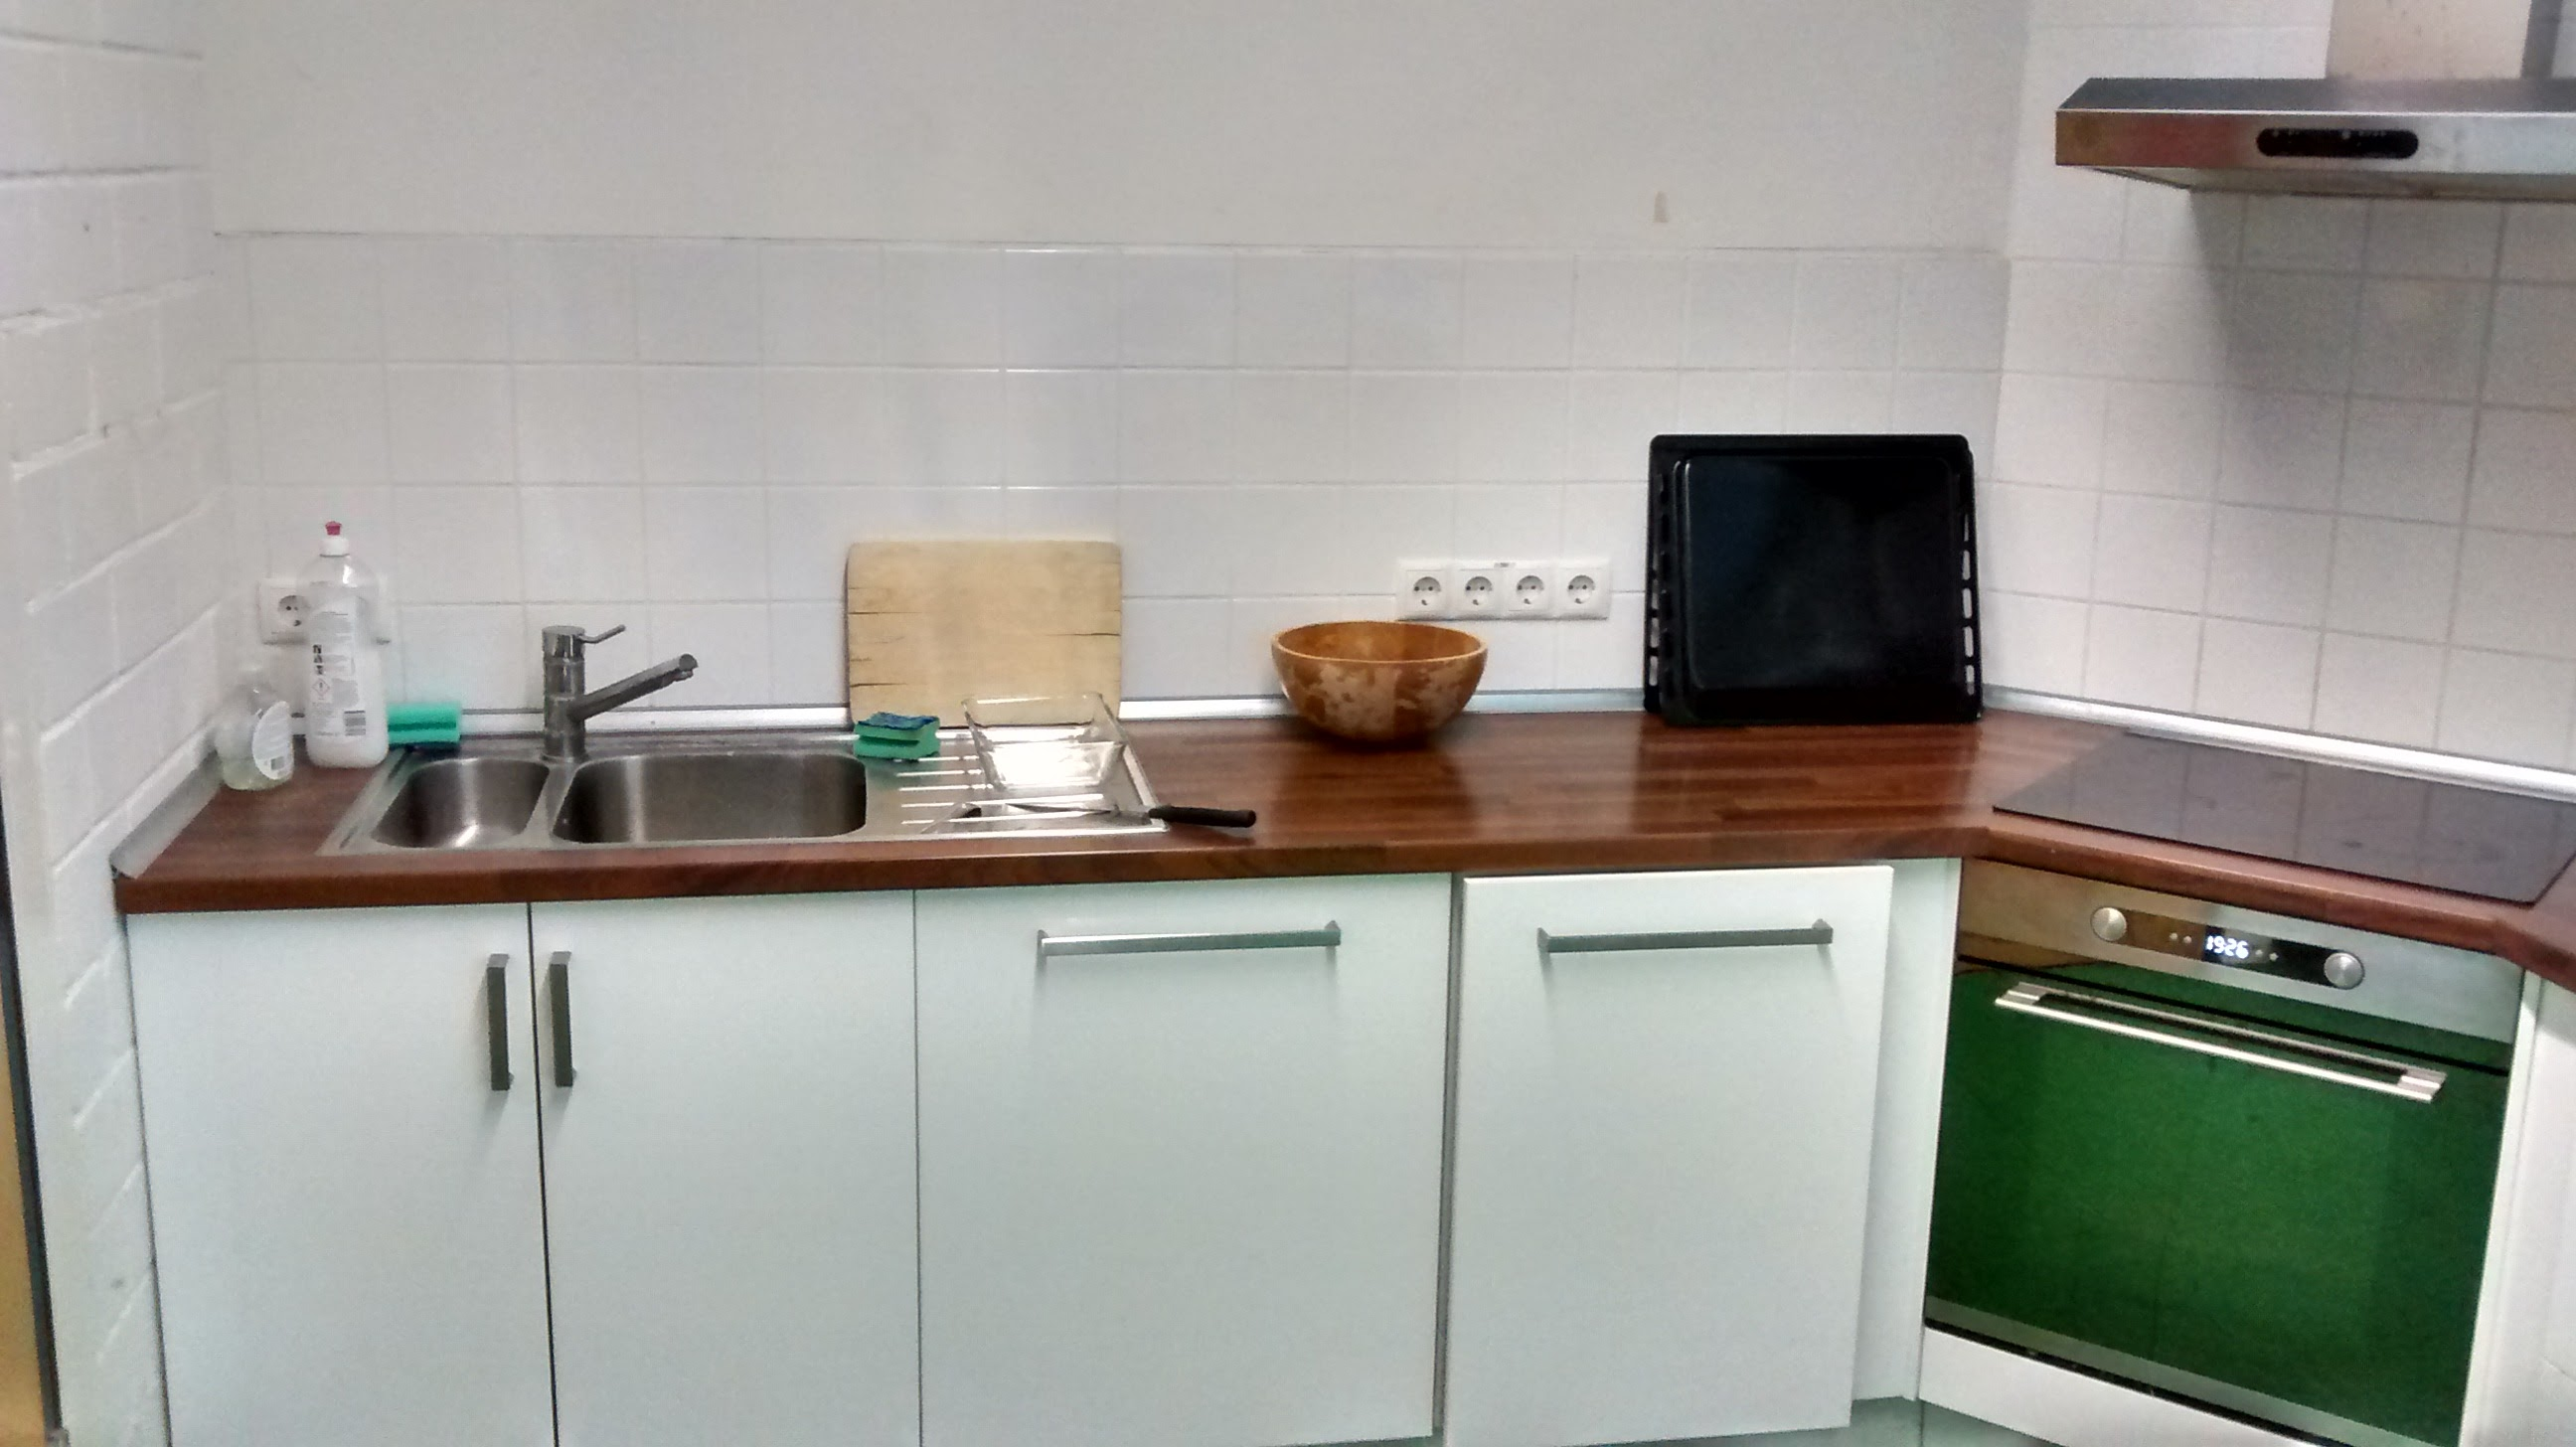
\includegraphics[width=\textwidth]{images/stove.jpg}
        \caption{Stove}
        \label{fig:stove}
    \end{subfigure}
    ~ %add desired spacing between images, e. g. ~, \quad, \qquad, \hfill etc. 
    %(or a blank line to force the subfigure onto a new line)
    \begin{subfigure}[b]{0.3\textwidth}
        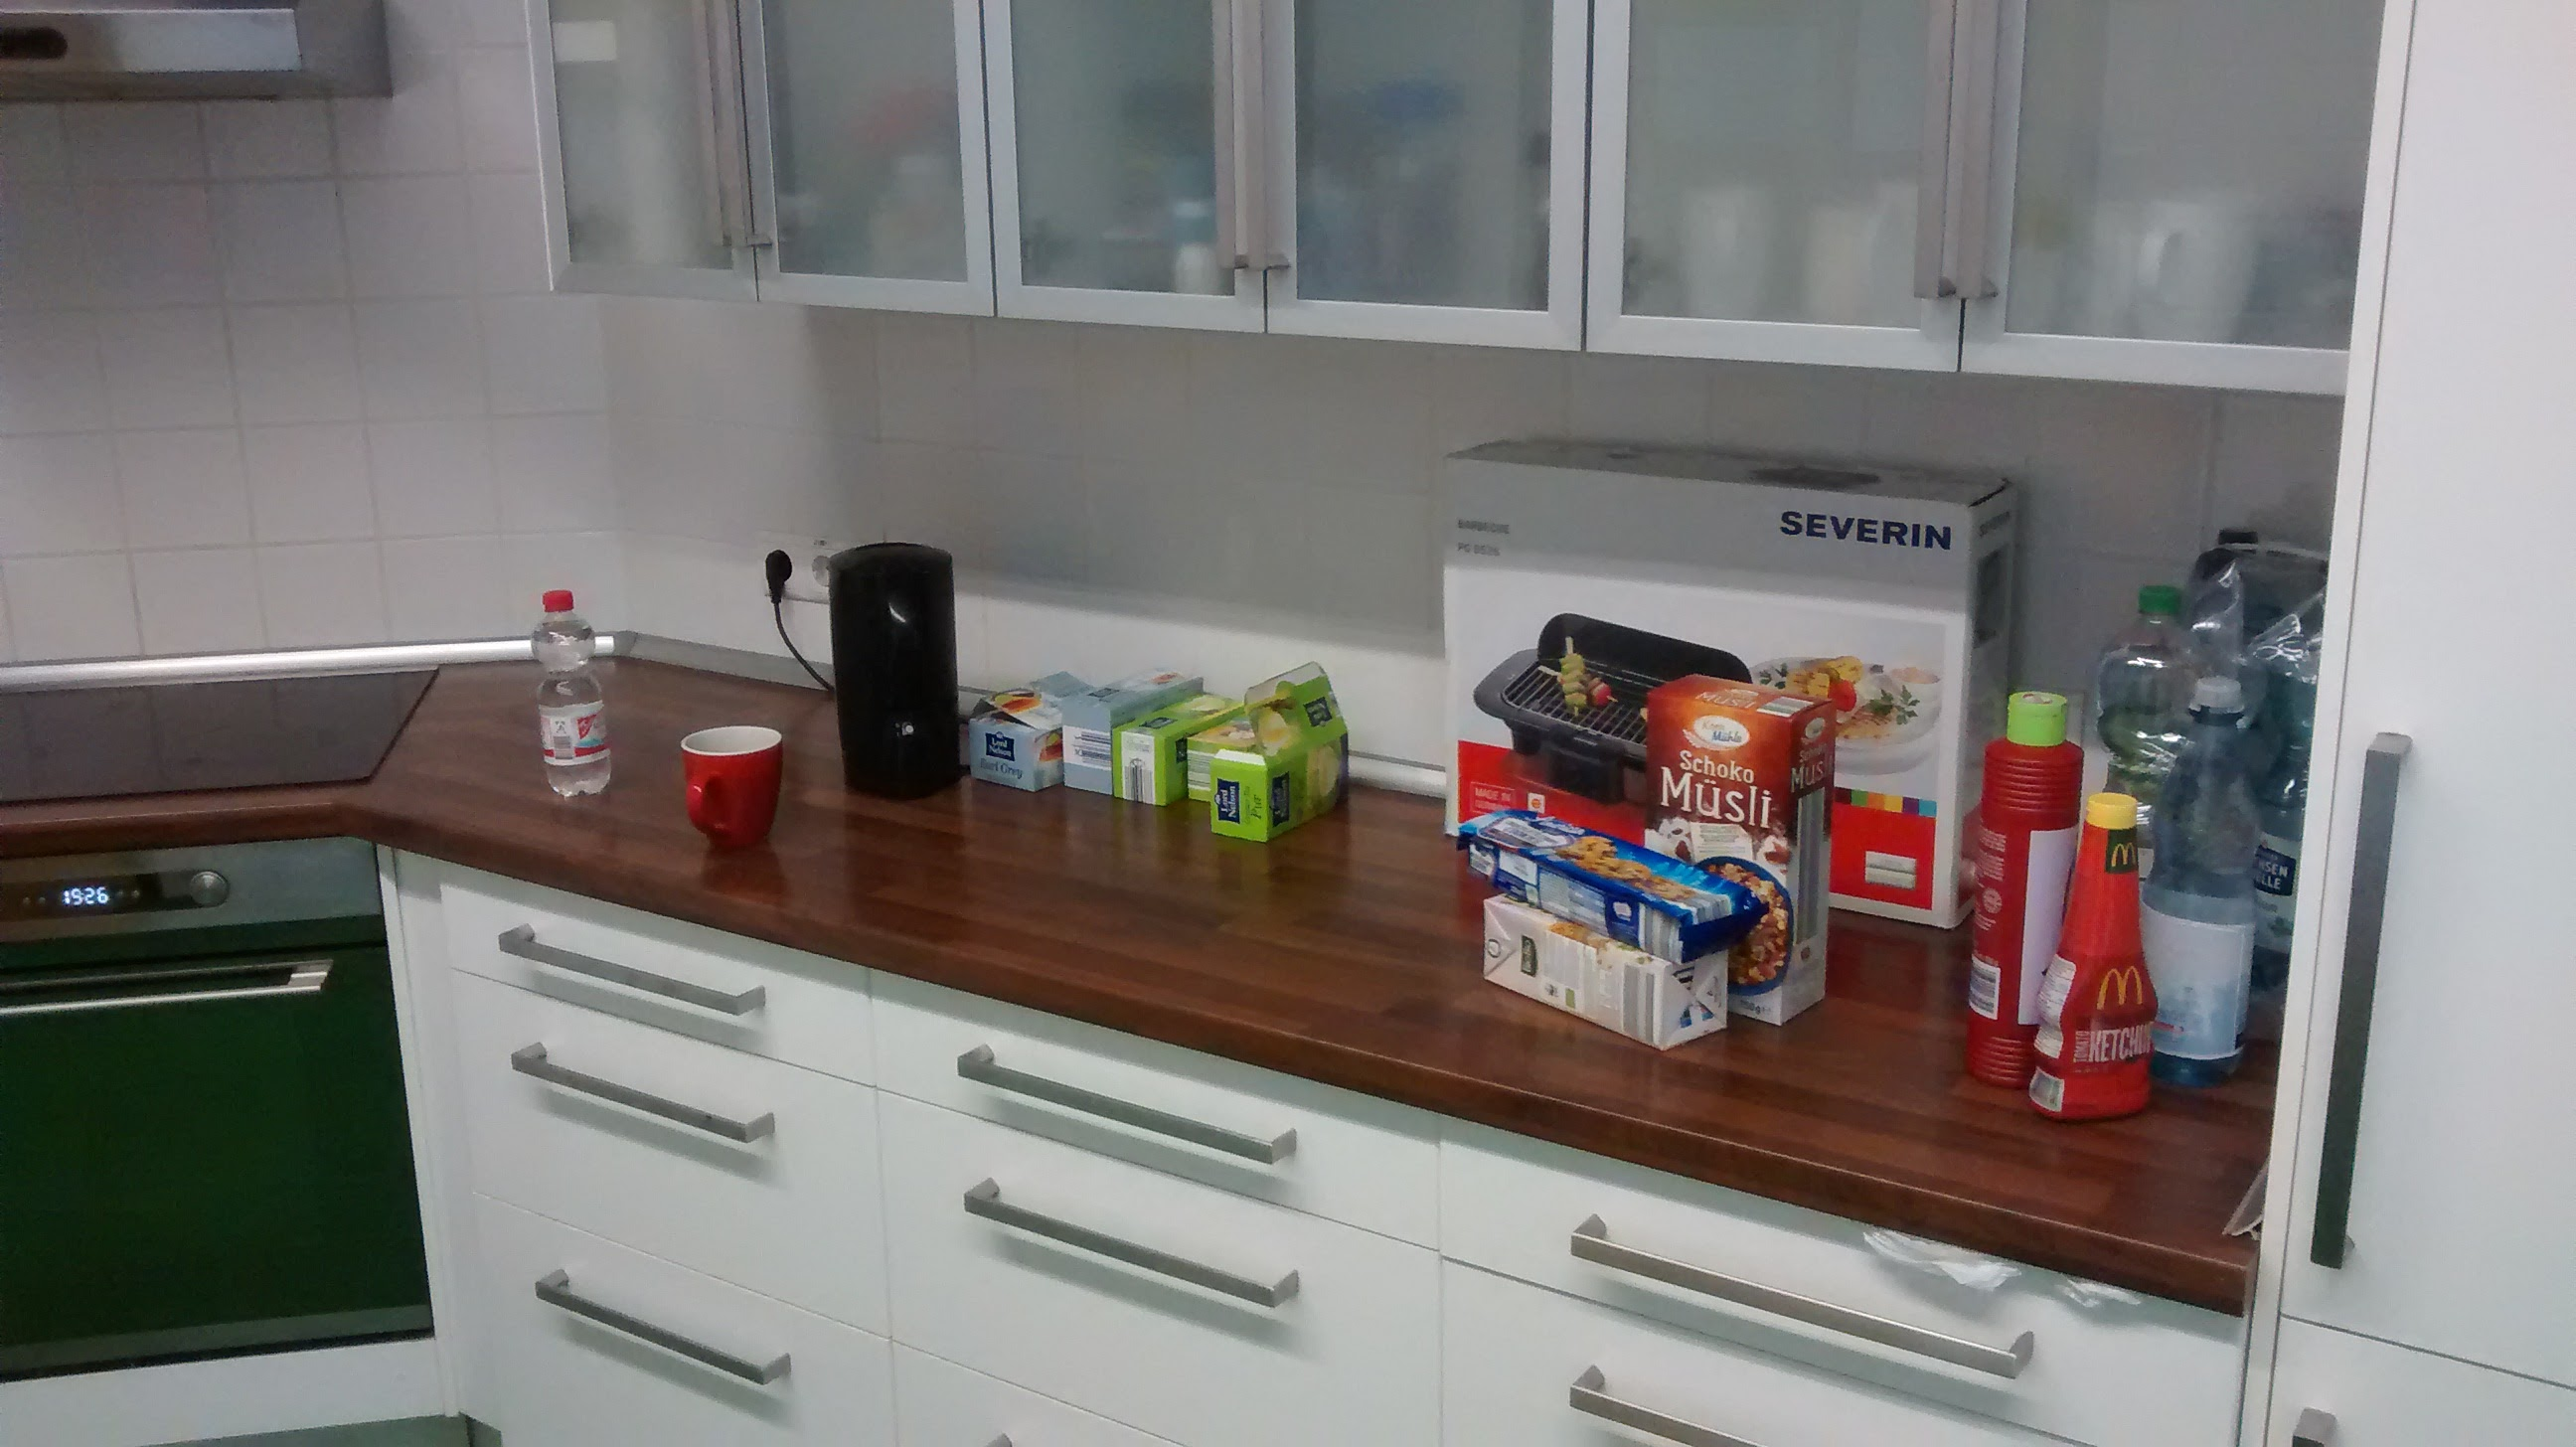
\includegraphics[width=\textwidth]{images/counter-top.jpg}
        \caption{counter-top}
        \label{fig:counter-top}
    \end{subfigure}
    \caption{Different possible object locations}\label{fig:alllocations}
\end{figure}


Thus models are developed which on absence of information of an object at a particular location decreases the probability of finding the object at that particular location while increasing the probabilities for other locations.


\FloatBarrier
\section{Dirichlet-Categorical-Bernoulli model}

For incorporating the absence observations we extended the Dirichlet-Categorical model  with a Bernoulli distribution.
In chapter \ref{} patterns in a single location were learned using a Beta-Bernoulli model, in chapter \ref{} we introduced the Dirichlet-Categorical model which could reason about multiple locations in single model, here we combine both the models. The Beta-Bernoulli model has the capability to learn from both success and failure results, this capability is added to the Dirichlet-Categorical model using a mixture node. 

The Bernoulli-trick is one way of making negative observations for certain location reduce its chances while making equally likely for the other locations. Thus, the location on which the object is not found are filtered out as impossible and the others are equally likely. The graphical diagram of the model is explained in \ref{dcbm}

The model is an extension as explained in \ref{sec: HDCM} . We combine a Bernoulli node $\gamma$ with the categorical node $x$. The Bernoulli is also an observation node as the categorical node. The observations are fed to the model to both the Bernoulli node and the categorical node. Suppose there are 3 locations where a object can be located. For a positive observation of locating the object at a location we feed [1.0 , 0.0, 0.0] to the Bernoulli node, where 1.0 represents object found at at location. For a negative observation i.e. the object not being found at a location the Bernoulli is given [0.0, 0.5, 0.5], where 0.0 signifies that no data was observed whereas the 0.5 increases uniformly the chances in the other locations.


\noindent
\begin{figure}[htp]
\qquad
\begin{minipage}{0.3\textwidth}
\centering

\tikz {
\node [const]                   (alpha) {$\alpha$};
\node [below=of alpha, latent]  (beta)  {$\beta$};
\node [below=of beta, latent]   (theta) {$\theta_i$};
\node [below=of theta, obs]     (x)     {$x_{ij}$};
\node [right=of x , xshift=0.05cm, obs]      (gamma) {$\gamma_{ij}$};
\edge {alpha} {beta};
\edge {beta} {theta};
\edge {theta} {x};
\edge {gamma} {x};
\plate {trials} {(x)(gamma)} {j location};
\plate {bags} {(theta)(x)(gamma)(trials)} {i time};
}

\end{minipage}%
\begin{minipage}{0.7\textwidth}

\begin{equation*}
	\alpha = <1, 1, .... , 1 > 
\end{equation*}
\begin{equation*}
	\beta \sim Dirichlet(\alpha)
\end{equation*}
\begin{equation*}
	\theta_i  \sim Dirichlet(\beta)
\end{equation*}
\begin{equation*}
	\gamma_{ij}  \sim Bernoulli(k)
\end{equation*}
\begin{equation*}
	x_{ij} \sim Categorical(\theta_i)
\end{equation*}
\end{minipage}

\caption[Dirichlet Categorical Bernoulli graphical model]{Graphical model representation of Dirichlet Categorical Bernoulli model. The boxes are ``plates" representing replicates. The outer plates represents hours of a day, while the inner plate represents if object was observed at the location each hour.}
\label{dcbm}
\end{figure}



\section{Experiments}

The goal of the experiments was to verify the performance of the proposed model with the HDCM introduce in \ref{}. 


The goal of the experiments was to comparatively evaluate the proposed method with the HDCM introduced in \ref{}, based on the number of experiments. For this we created a simulated dataset with known ground truth distributions. The observations were then by the models to learn the latent probabilities. The learned probabilities were then compared with the ground truth. The above experiments were run 
\subsection{Simulated Dataset: Kitchen Object Dataset}

To demonstrate the proposed approach we have generated a kitchen object dataset. The dataset consist of observations(presence and absence) of a cup in a kitchen environment made by a domestic robot. The robot can scan 4 locations in the kitchen: sink, counter-top, stove and cabinet. The time of the scan is discretized into 3 times of the day: morning, afternoon and night. 

The generative process for each possible observation(present and absent) in the dataset 
\begin{itemize}
    \item Choose $ \theta \sim Dirichlet(\alpha)$ (Distribution of object over location-time)
    \item Choose randomly the time period $i$.
	\item Choose the location $x_n$ $\sim$ Categorical$(\theta_i)$
	\item Choose the presence of object $p_n$, in time period $i$ and location $x_n$  $p_n$ $\sim$ Bernoulli$(\beta) $
\end{itemize}

Ground truth of the distribution in the object location distribution over time in shown in Figure \ref{absent-gt}.


\begin{figure}[htp]
\centering
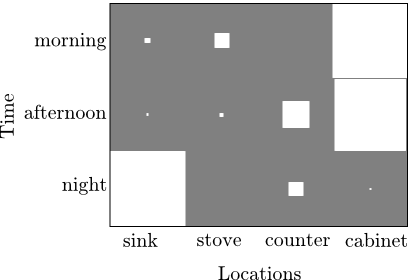
\includegraphics[width=0.6\textwidth]{images/absent_groundtruth.png}
\caption[Simulated object location ground truth distribution]{Simulated object location ground truth distribution.
The x-axis represents the locations the y axis represents the timezones. The size of the white box indicates the probability of the object presence.}
\label{absent-gt}
\end{figure}

From the ground truth we can observe that there is higher probability to find the object in the sink during night time and in the cabinet during the other time periods. We need to develop models which can learn these temporal patterns from the observations

\section{Evaluation}

\todo[inline]{TODO}

We compare the Dirichlet-Categorical-Bernoulli model with the Hierarchical-Dirichlet-Categorical model explained in \ref{sec: HDCM}. We compare the ground truth dirichlet probabilities, used to generate the simulated dataset and the learned probabilities and evaluate the performance of the learning. 
We use the adopted  Bhattacharyya distance \cite{rauber2008bhattacharyya} to quantify the similarity between the simulated and the learned Dirichlet distribution.
\begin{figure}
    \centering
    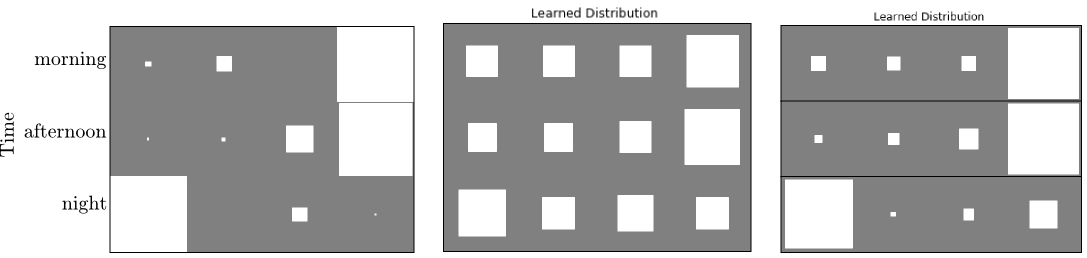
\includegraphics[width=\textwidth]{images/absent_learned.png}
       
    \begin{minipage}[t]{.35\textwidth}
    %\centering
    \subcaption{Ground Truth}\label{fig:absent-gt}
    \end{minipage}%
    \begin{minipage}[t]{.3\textwidth}
    %\centering
    \subcaption{HDC model}\label{fig:absent-hdcm}
    \end{minipage}
    \begin{minipage}[t]{.25\textwidth}
    %\centering
    \subcaption{HDCB model}\label{fig:absent-hdcmb}
    \end{minipage}

\caption[Model Evaluation of HDC and HDCB ]{Model Evaluation: \ref{fig:absent-gt} is ground truth of the distribution. \ref{fig:absent-hdcm} is the learned distribution using the HDC model. \ref{fig:absent-hdcmb} is the learned distribution using the HDCB  model }
        \label{fig:absent-eval}
    
\end{figure}


\begin{figure}[htp]
\centering
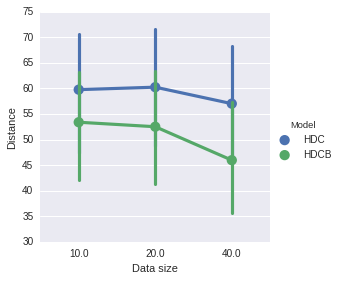
\includegraphics[width=\textwidth]{images/bhatta-distance.png}
\caption[Model evaluation : Bhattacharyya distance]{Bhattacharyya distance between the ground truth and the learned distributions for different size of training data. }
\label{}
\end{figure}




\chapter{Knowledge-enabled Fault Tolerant Search}
\label{cha: search}

All the previous chapters have explained the process of knowledge generation from information gathered by the robot, in this chapter we would like to provide a motivating example of using this knowledge by the robot to make smart decisions. The problem we like to solve is to find people or objects in domestic environments, with the added information that the available vision detectors are faulty. Robots use sensors like camera, laser scanners, tactile sensors  to recognize objects and persons. While vision based object and person recognition is one of the most widely studied topics in artificial intelligence, even the best detectors still encounter failures. Most of the state-of-art detectors are based on machine learning methodologies. These detectors always publish their \emph{detection probability}. The detection probability quantifies the success rate of recognizing an object or person. This chapter explores methods of using our learned location probabilities and detection probabilities to accomplish a search task more efficiently in a domestic environment. 


Efficient searching for objects in the environment is one of the application for the knowledge being learned from object locations. The learned knowledge about location probabilities can be used as heuristics to improve the search time of objects. There are 2 basic methods in which we can use the learned knowledge as heuristics, first we can search for objects in the decreasing order of the learned probabilities or alternatively we can use the generative model to predict based on its learned probabilities. However the probabilistic representation of the learned knowledge can be used in ingenious way to solve more complex problems. 

\begin{figure}[htp]
\centering
\begin{subfigure}{.4\textwidth}
  \centering
  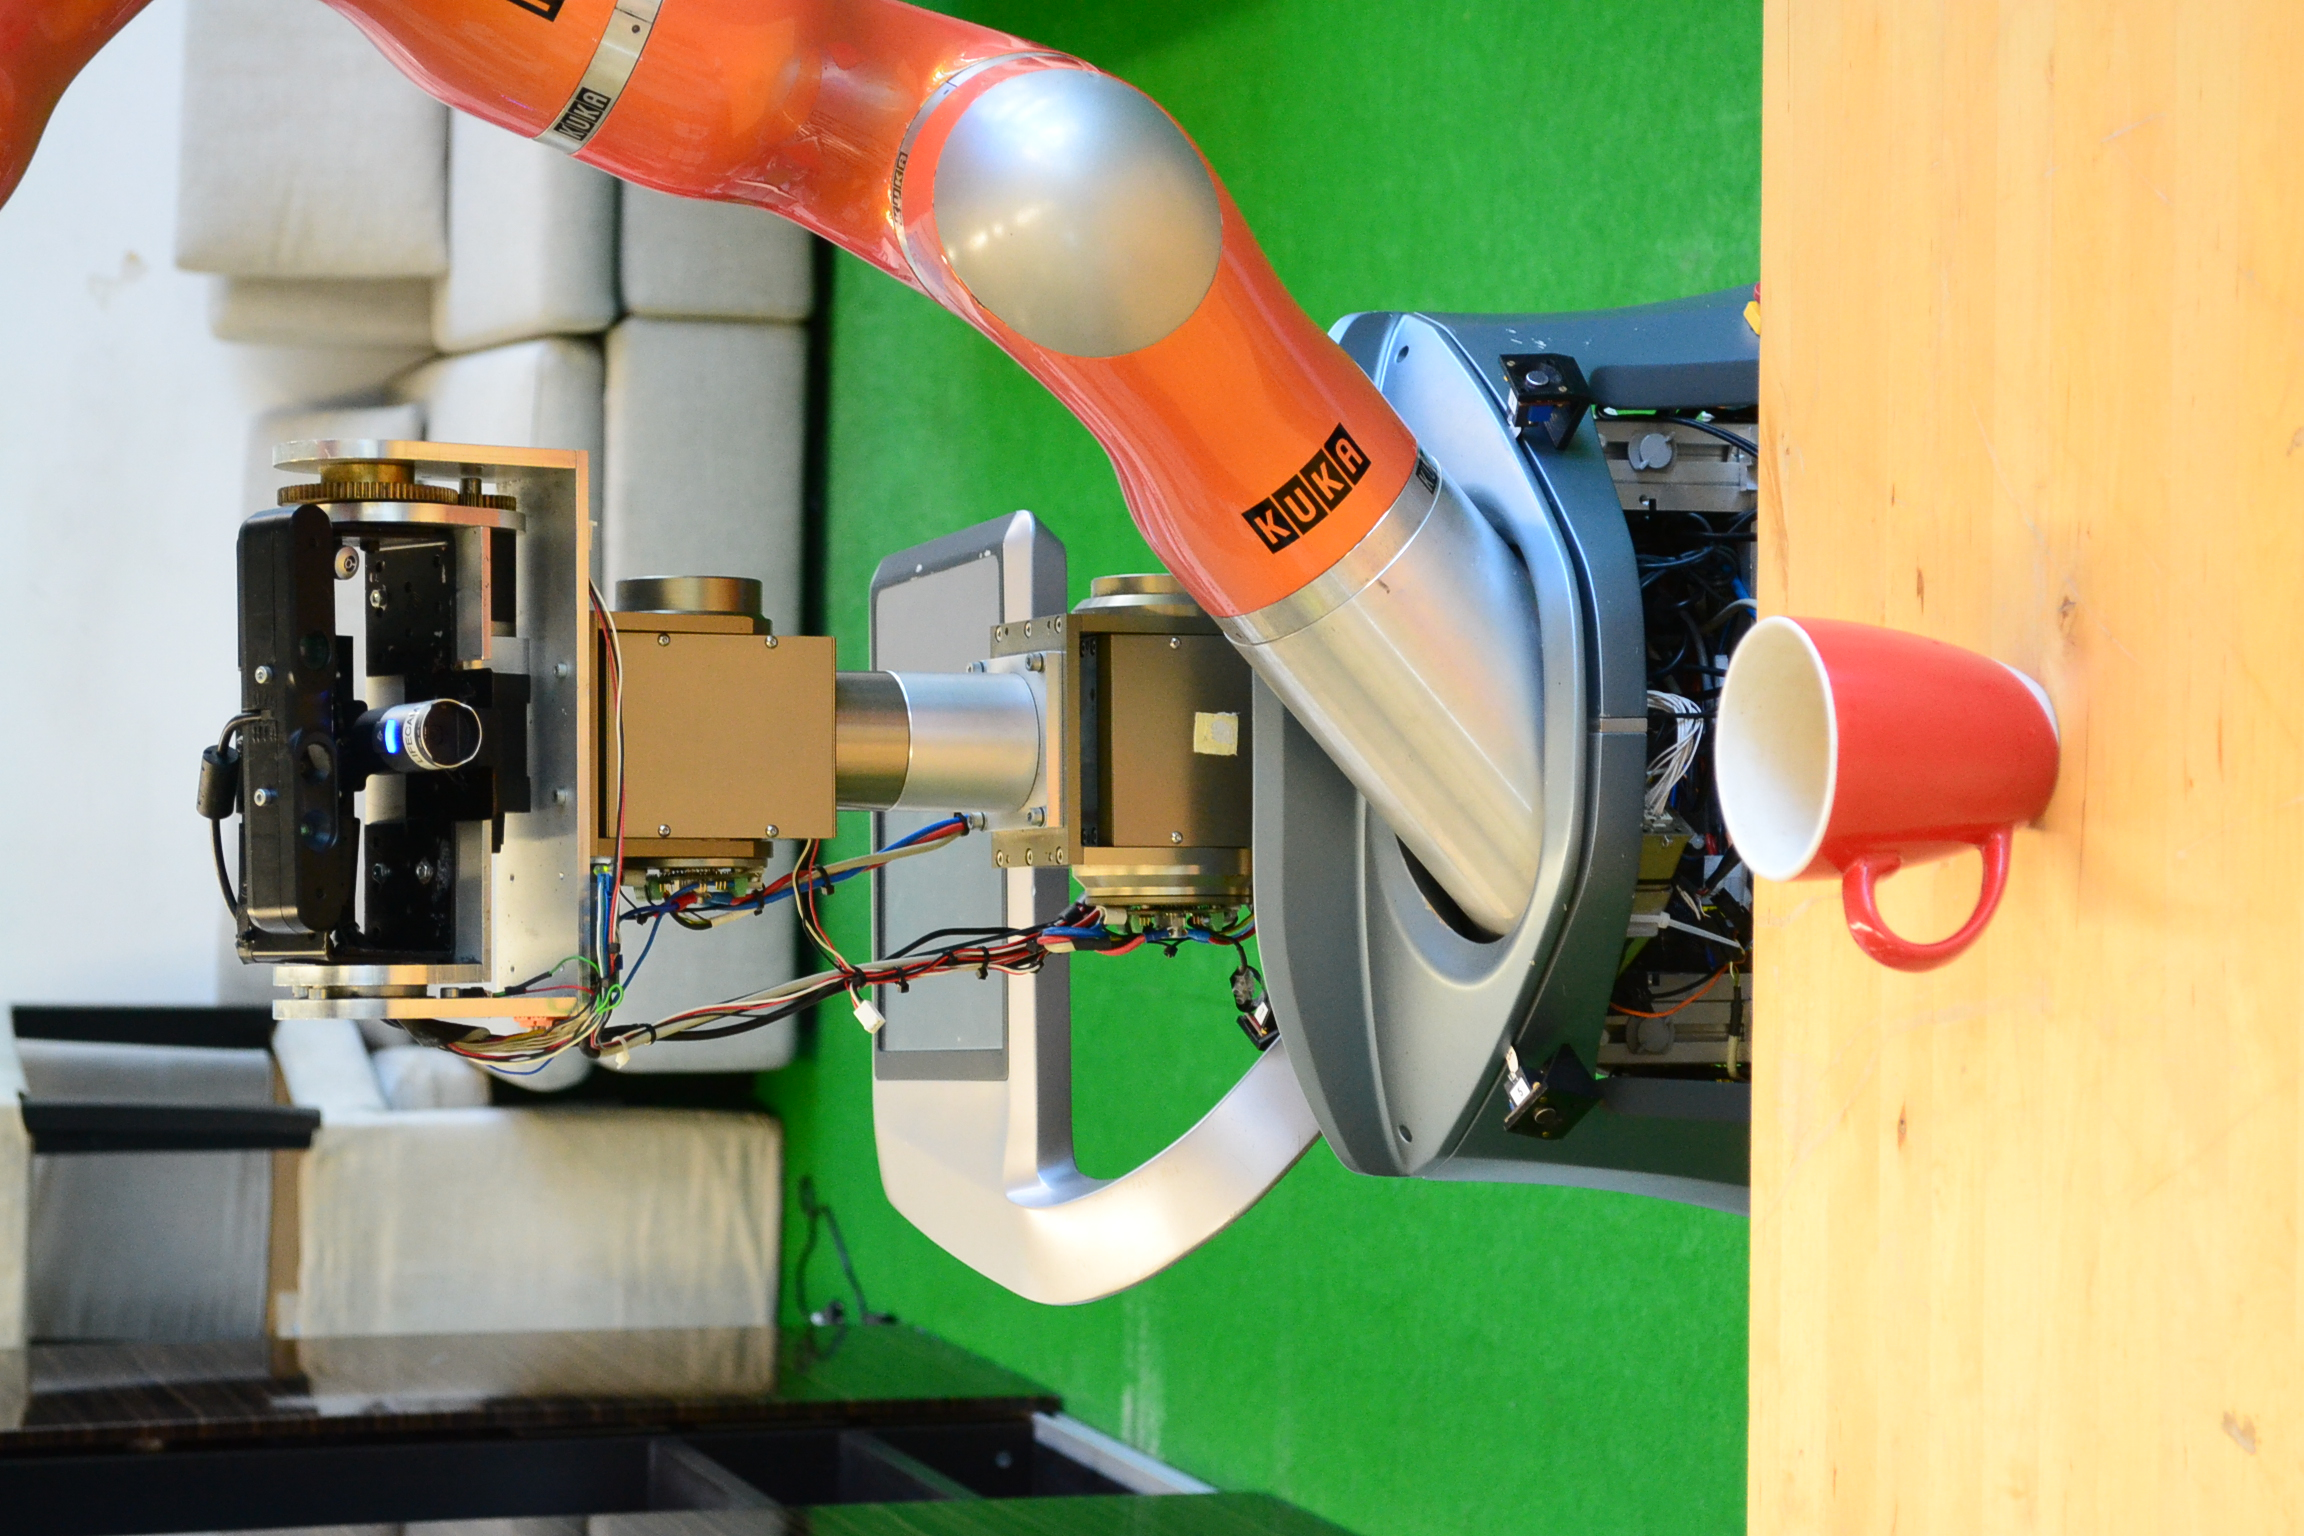
\includegraphics[width=0.9\linewidth, angle=-90]{images/robot_looking_cup.jpg}
\end{subfigure}%
\begin{subfigure}{.6\textwidth}
  \centering
  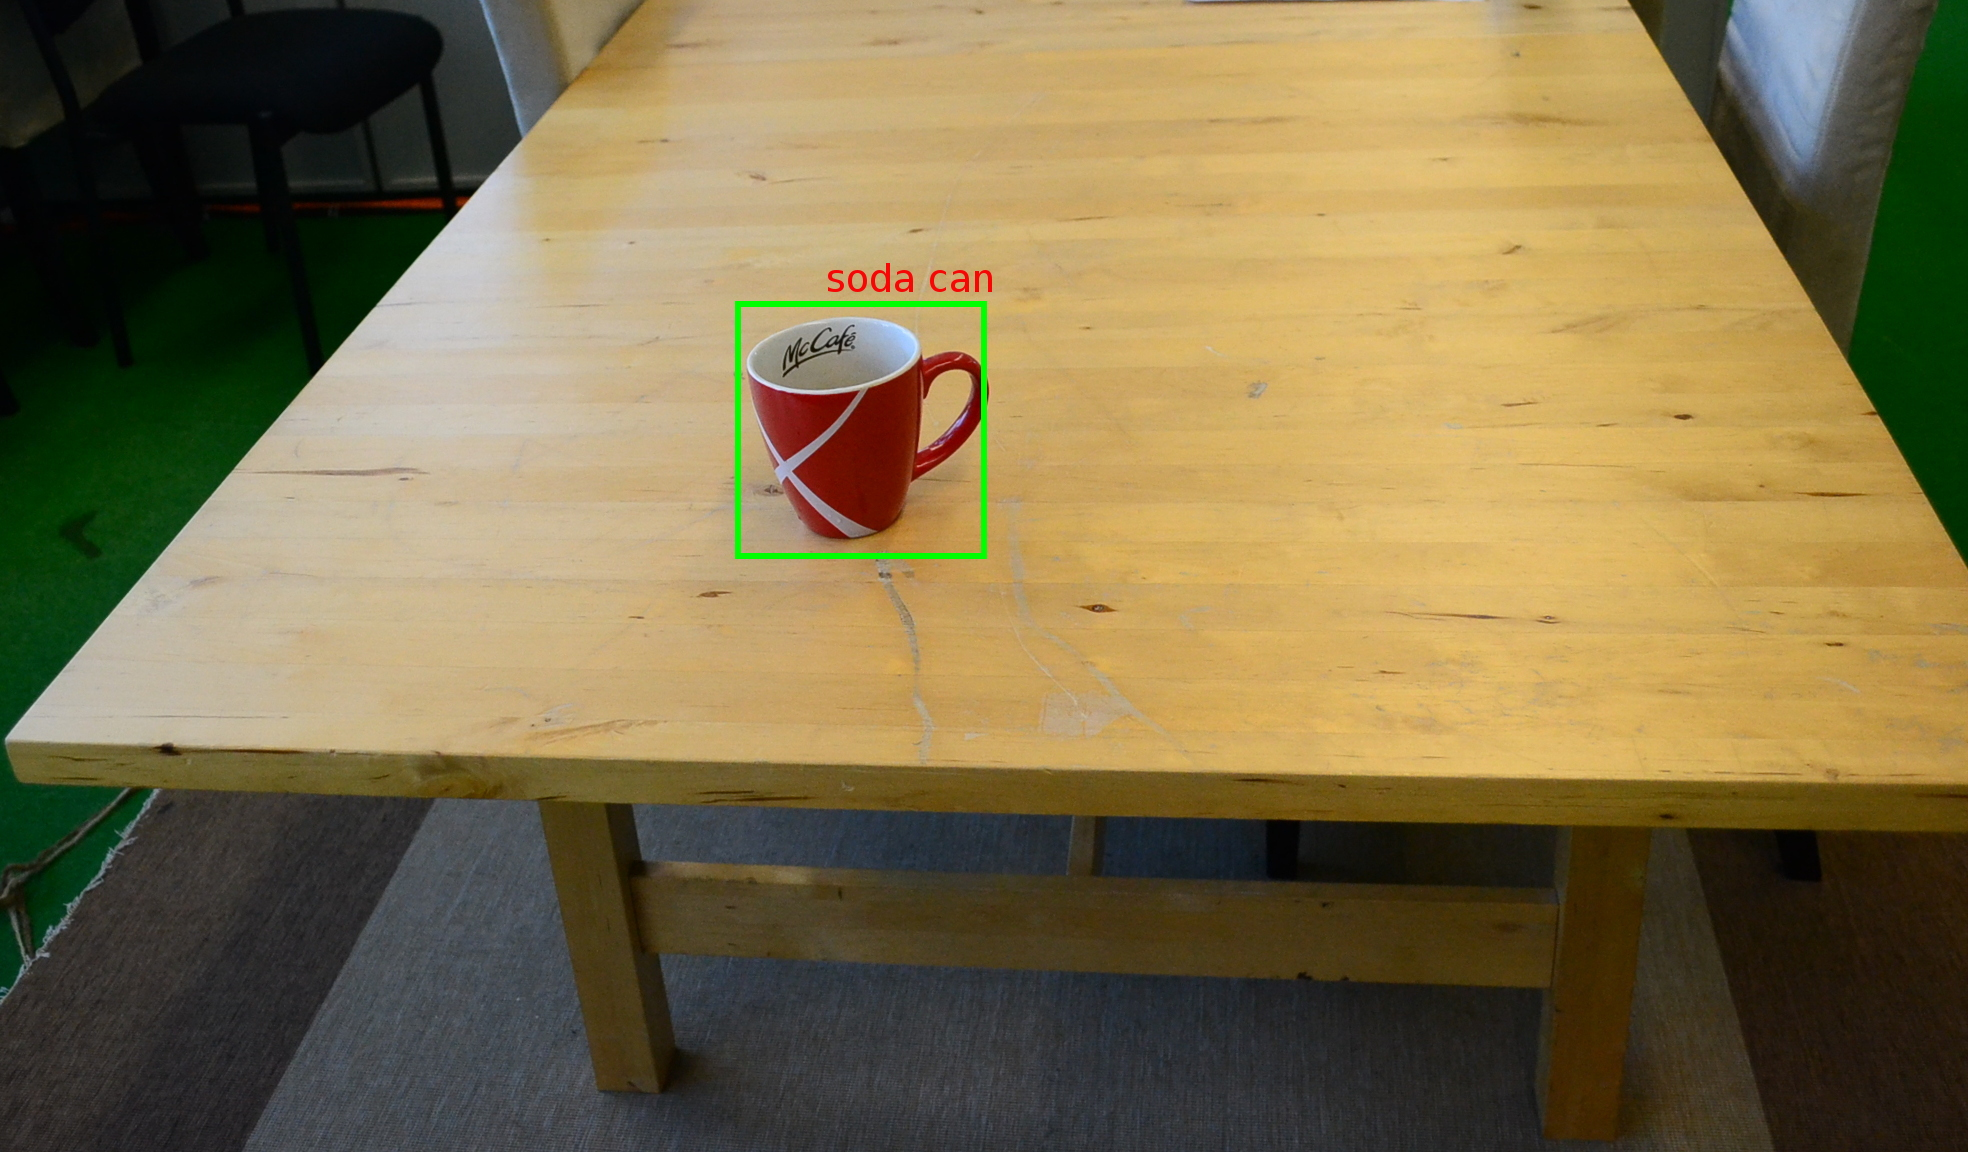
\includegraphics[width=\linewidth]{images/robot_view_cup.jpg}
\end{subfigure}
\caption[Fault tolerant search example]{Failures in object detection. The cup is misclassified as a soda can}
\end{figure}

In robotics \cite{chung2007decision} formulated the search control problem as a decision-making problem. This formulation of the search problem can include the information of false alarms and false detection. \cite{roy2003planning} demonstrated a system of finding people in a health care setting using a state probabilities of the people in a Partially Observable Markov Decision process planner. 

The above mentioned researchers have demonstrated how probabilities about locations can be used to make more informed decisions for the search problem. We here illustrate how the learned probabilities can be used to develop a \emph{sequential decision search algorithm} which can accommodate the recognition failure of the vision algorithms. The proposed algorithm here combines both the \emph{detection probability} and the \emph{learned probability} of the objects and provides sequential decisions for the next location to search.

\section{Probabilistic Search}

The robot is assumed to begin with map of the environment, learned knowledge as a probability distributions over where the people and objects might be located and the detection probability for each object and person. The robot can move around in the environment to look for the person or object, perceives the environment. 
The idea is to use the learned knowledge of the object locations as the first guess (prior ) of the probabilities that the object in question is located in each of the possible object locations \cite{cressie2015statistics}. The prior probabilities suggest which location to search first. If the object is not found in that location, the prior probabilities are then updated (yielding the posterior), and the process is repeated until the object is found. 

The following problem formulation is from \cite[p. 25]{cressie2015statistics}.
Assume that the domain of interest is a home we call $D_s$, which is made up of n spatial areas. Let $Y_i = 1$ if the object is in the \emph{i}th location, and then $Y_i = 0$ if it is not; $ i = 1, .... , n$. Now as discussed above object detectors can fail to detect the object. So, let $Z_i = 1$ if the object is found in the \emph{i}th location, and $Z_i = 0$ if not.

We can define two terms \emph{detection probability} ,
\begin{equation}
	p_i = Pr(Z_i = 1| Y_i =1), \qquad  i = 1,...,n,
\end{equation}
which is a conditional probability, and the \emph{occurrence probability},
\begin{equation}
	\pi_i = Pr(Y_i = 1),\qquad  i = 1, .... , n.
\end{equation}

This can be expressed in probabilistic programming form:
\begin{gather}
	Z_i | Y_i \sim Bernoulli (Y_i, p_i), \qquad  i  = 1,....,n \\
	Y_i \sim Bernoulli(\pi_i),\qquad   i = 1,...,n,
\end{gather}

where, the occurrence probability {$\pi_i$} is given by the learned probabilities, while the detection probability {$\pi_i$} is provided by the object detector algorithm.

Now, assume that hte \emph{i}th location is searched by the robot and the object is not found (i.e., $Z_i = 0$). In that case, the probability that the object is in the \emph{i}th location is updated using Bayes' Theorem. This yields the posterior probability,

\begin{gather*}
	Pr(Y_i = 1 | Z_i = 0) = \frac{Pr(Z_i = 0|Y_i=1)Pr(Y_i=1)} {Pr(Z_i=0)} \\
	                       = \frac{Pr(Z_i = 0| Y_i =1 )Pr(Y_i =1)}{Pr(Z_i=0|Y_i =1)Pr(Y_i = 1) + Pr(Z_i=0|Y_i=0)Pr(Y_i=0)} \\
	                       = \frac{(1 - p_i)\pi_i}{(1 - p_i)\pi_i + (1)(1 - \pi_i)} \\
	                       = \frac{(1 - p_i)\pi_i}{1 - p_i\pi_i}
\end{gather*}

where we assume that there are no false-positive detection (i.e., $Pr(Z_i =0| Y_i = 0) = 1$). Note that the new posterior is less than the prior probability $\pi_i$ as the object was not observed.

Since the object is not found in the searched location, then this should also affect the posterior probability in the other grid boxes. For example, consider the \emph{j}th location, where $j \neq i$. Then,
\begin{align*}
	Pr(Y_j = 1 | Z_i=0) &= \frac{Pr(Z_i = 0 | Y_j = 1)Pr(Y_j = 1)}{Pr(Z_i = 0)} \\
	                    &= \frac{\pi_j}{ 1 - p_i\pi_i}
\end{align*}

Thus, the posterior probability of the object being the \emph{j}th location is greater than the prior probability $\pi_j$ . These new posteriors will then become the next prior probabilities is a sequential procedure that would determine the next location to search.


\section{Example}

We illustrate a scenario and demonstrate how the robot performs its search based on two different search methodologies when there is fault caused by the object detector. The proposed probabilistic search is compared with a simple search method. Our aim is to find out the how by using probabilistic search the robot is making better search decisions in the presence of the fault.

We consider the scenario of a domestic robot in a home which is searching for an object. The robot has been in the home for long enough and made some observations. The robot has learned that the cup can be found 3 locations in the home, thus the domain for search can be defined as $D_s = \{cupboard, table, dishwasher \}$ . Based on these previous observations it also learns the occurrence probabilities as $p_i = \{ 0.8, 0.1, 0.1\}$ . Currently the cup is located in the cupboard \ref{fig:cup_in_cupboard} and the robot is asked to fetch the cup, so the robot searches the cupboard as its the most likely location based on prior beliefs. But the detector algorithm is not able to detect the cup and provides a faulty observation of the cup not found. 

We test the scenario using our proposed methods with 2 different detection probability

\begin{figure}[htp]
\centering
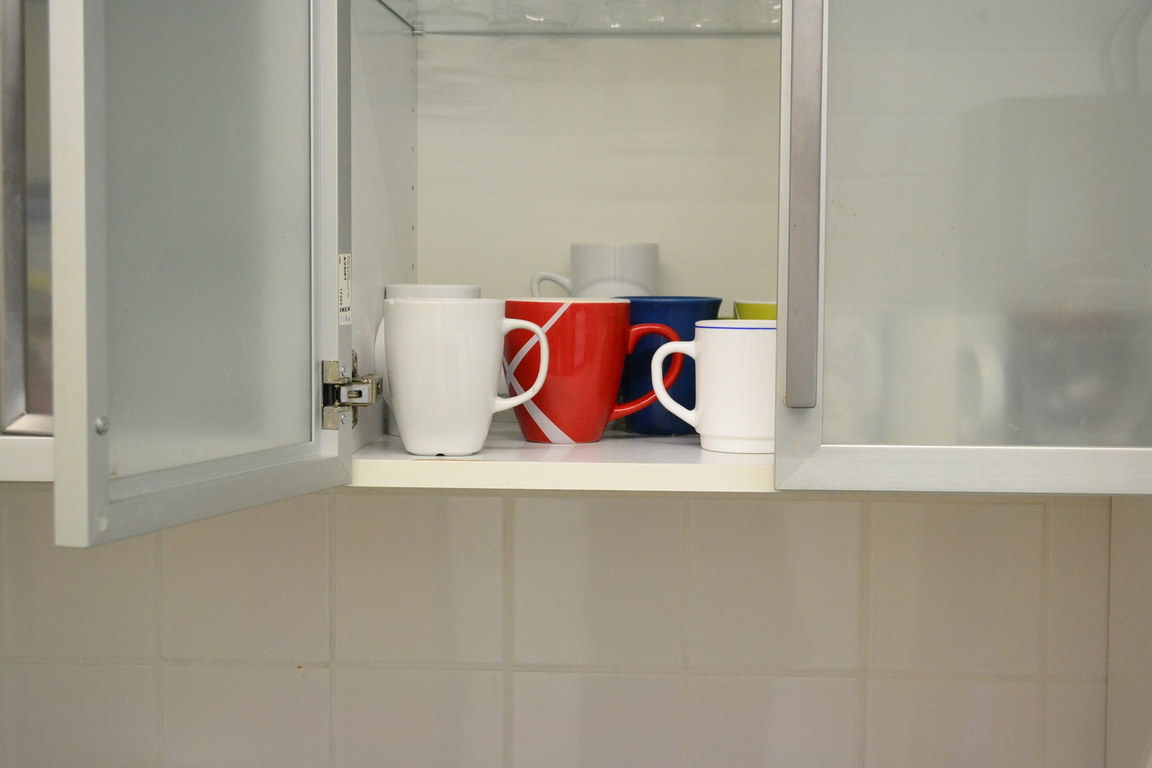
\includegraphics[width=0.4\textwidth]{images/cup_cupboard.jpg}
\caption[Probabilistic search example]{Example scenario of finding the cup which is located in the cupboard. The object detector is not able to recognize the object because of occlusion}
\label{fig:cup_in_cupboard}
\end{figure}

\begin{figure}[htp]
\centering
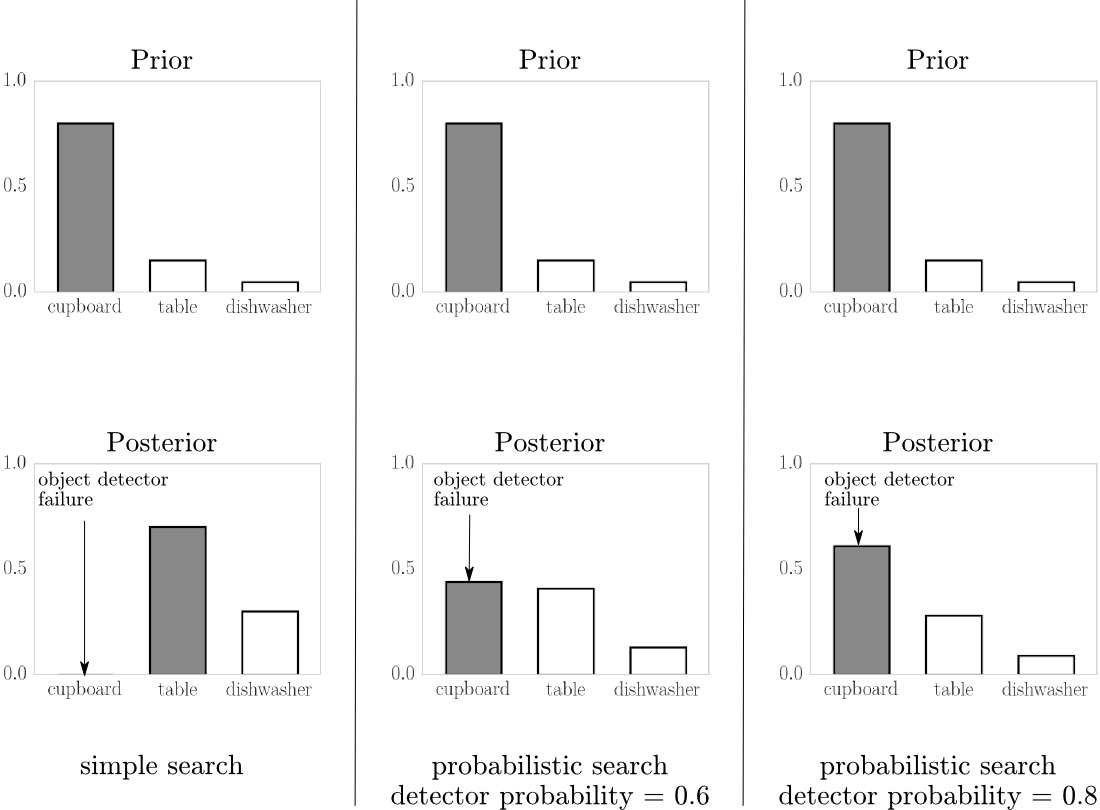
\includegraphics[width=\textwidth]{images/search.png}
\caption[Probabilistic search scenario]{The upper graphs shows the robots prior belief of the possible locations where the cup can be found. These beliefs at the outset have the probabilities which were previously learned by the robot. The shaded bar corresponds to the next location the robot will search. The lower-left graph shows the posterior probability(updated belief of the robot), when the detector fails to detect the object at the cupboard. Each column represents the change in belief based on the different search methods and detection probability. In probabilistic search the robot still has the belief that the cup is present in the cupboard while in simple search the robot will search the next location}

\label{fig:search_results}
\end{figure}

 
\subsection{Simple Search}

In simple search the robot goes to the highest probable location and on inability to find the object go to the next highest probable location. The search ends if the object is found or when the robot scans the least probable region. Thus in the above scenario the robot will first scan the cupboard if it finds the cup then it goes ahead and executes its task. If the robot fails to detect the cup in the cupboard it reduces the locations probability to $0$ and moves to next locations. Thus the default search sequence will be ${cupboard, table, dishwasher}$

\subsection{Probabilistic search}

Figure \ref{fig:search_results} illustrates probabilistic search algorithm. The heights of the bars in the graphs indicate the possibility of finding the object at the particular location. The upper graphs of Figure \ref{fig:search_results} shows that the prior beliefs of the robot which it had learned. As per the prior the robot is highly believes that the cupboard is the most likely place to search for the cup. The shaded bar in each graph represents the next location the robot will scan based on its current belief. So the robot goes ahead and scans the cupboard but the detector fails to detect the object. Now based on this new observation the robot goes ahead and re-allocates its belief. This re-allocated distribution is called the posterior distribution. The lower graphs in Figure \ref{fig:search_results} represents the posterior distribution after taking into account that the detector didn’t find the cup in the cupboard. Each column of the Figure \ref{fig:search_results} represents the different methods based on which the posteriors are updated. The first column is based on simple search which does not considers the detector probability. The middle column uses an object detector with 60\% detection probability, while the last column uses an object detector with 80\% detection probability. For the simple search the posterior has $0$ probability for the cupboard. Thus the robot has completely believed the object detector and considers that the object is not present in the cupboard, therefore as per the posterior the robot now moves to the next probable location. However, in probabilistic search the posteriors probability of cupboard is reduced , but not completely to $0$. As a result it still believes that the cup is present in the cupboard and tries again to search the cup in the cupboard. The reduction in the posterior probability of cupboard depends on the detector probability. 

This illustrates that the probabilistic search understands the limitation in the object detector and updates its beliefs to accommodate this limitation and make better \emph{informed} decisions.  


\section{Discussion}
In this chapter we proposed an approach that enables the robot combine the knowledge learned by robot about object location and the knowledge about the object detector, for making search decisions. Our approach uses Bayesian methods to incorporate the knowledge about the object detectors to make better search decisions. Furthermore with an illustrative example we showed how the robot makes knowledgeable decisions even when with false information from the object detector.
% chapter  (end)
\chapter{Conclusions}
\label{cha:}


We believe as and as robots become more autonomous, the robot will be able to record more and more obserations. This will help the approaches discussed in the thesis to be more accurate and make better predictions.
 create a behavioural map of the house and its occupants, including room function and occupancy modelling, household activities and routines.

Uncover habits and predict human behaviour 


enhance the quality of life by  ... 

All models are developed with the user at the center. 

All the models were developed using probabilistic programming languages 


We have demonstrated the  powerful aspects of model-based machine learning is the ability to extend the model to take account of more complex situations. 
Model was first developed for learning from single location,  which was extended to model which could learn multiple locations. 
\section{Future Work}


% chapter  (end)
% bibliography and appendixes
%%%%%%%%%%%%%%%%%%%%%%%%%%%%%%%%%%%%%%%%%%%%%%%%%%%%%%%%%%%%%%%%%%% 
%                                                                 %
%                           BIBLIOGRAPHY                          %
%                                                                 %
%%%%%%%%%%%%%%%%%%%%%%%%%%%%%%%%%%%%%%%%%%%%%%%%%%%%%%%%%%%%%%%%%%% 
 
%This method produces a numbered bibliography where the numbers
%correspond to the \cite commands in the text. See the LaTeX manual.
%\specialhead{\bibname}

\bibliographystyle{apalike} % mit Buchstaben
%\bibliographystyle{newapa} % mit Buchstaben
%\bibliographystyle{plain} % normal
%\bibliographystyle{unsrt} % in reinfolge des Textes
%\bibliographystyle{abbrv} % wie plan , nur abgekürtz

\begin{singlespace}

\bibliography{proposal}

\end{singlespace}
   


%\emptypage
%\emptypage

\end{document}
